\documentclass{statsmsc}

\title{Robust Extreme-Value Anomaly Detection for Non-Stationary Streams}
\author{KATERYNA KAPLUNOVA}
\CID{06009246}
\supervisor{ZAK VARTY}
\date{21 August 2025}
%For today's date, use:
%\date{\today}
\logoimg{}

% THIS IS WHERE NEW COMMANDS CAN BE DEFINED

% commands below only used in the proof; otherwise can be deleted
\newcommand{\consta}{a}
\newcommand{\X}{X}
\newcommand{\EE}[1]{ \mathrm{E} [ #1 ] }
\newcommand{\inparenth}[1]{\left( #1 \right)}

\usepackage{xcolor}
\usepackage{hyperref}
\hypersetup{
    colorlinks,
    linkcolor={blue!50!black},
    citecolor={blue!50!black},
    urlcolor={blue!50!black}
}
\usepackage[bmargin=4cm]{geometry}

\makeatletter
\renewcommand*{\figureformat}{\figurename~\thefigure}
\makeatother

\begin{document}

% Generates the Title Page
\maketitle

% Generates plagiarism declaration
\declarationname{Kateryna KAPLUNOVA}
\declarationdate{28.08.2025}
\declaration 

\begin{acknowledgements}
    First and foremost, I want to thank my dad. He always believed in me and never stopped pushing me to go further than I
    thought I could. Losing him this summer was the hardest moment of my life, and for a while, it felt like my world had 
    stopped. But his belief in me gave me the strength to keep going and finish this thesis. I hope he would be proud. 

    I also want to thank my family, friends and my boyfriend for standing by me with patience and encouragement throughout this work. 
    I am grateful to my supervisor for his guidance and feedback, and to my research group for the helpful conversations 
    and support they shared along the way. This project would not have come together without them. 
\end{acknowledgements}

%=================================================================
% VERY IMPORTANT
% This command switches from Roman to Arabic numbering for main part of report. Do not modify.
\mainmatter
%=================================================================

\begin{abstract}
    This thesis investigates whether Extreme Value Theory (EVT), specifically the Peaks-Over-Threshold (POT) framework,
    can provide reliable anomaly detection in non-stationary streaming data. Unlike machine learning approaches that adapt
    flexibly but lack error-rate guarantees, EVT links alarms to probabilistic thresholds, yet its assumptions of weak 
    dependence and stationarity are rarely satisfied in real world streams.

    Two methodological extensions are examined in this study. First, an alternative preprocessing pipeline is introduced to 
    transform raw data into residuals that better approximate the weak-dependence assumptions required by EVT. This pipeline 
    combines exponential smoothing, rolling variance normalisation, and seasonal differencing to address common forms of 
    non-stationarity in streaming data. Second, the Expected Quantile Discrepancy (EQD) criterion is integrated for automated 
    threshold selection, replacing heuristic choices with a more principled approach. Their performance is assessed both 
    through a diagnostic framework of dependence and tail-model checks, and through event-based evaluation on three
    Numenta Anomaly Benchmark datasets (CPU, Twitter, and Traffic), each of which exhibits distinct forms of non-stationarity.

    Results show that preprocessing has complementary strengths but clear limits: EVT-based detectors only perform reliably 
    when residual extremes come close to independence, a condition
    that proves difficult to achieve in practice. The study further highlights that EQD is effective only when residual 
    extremes approximate independence, and that preprocessing alone sometimes cannot eliminate clustering, underscoring 
    the need for further work.

    Overall, POT-based detection remains feasible for streaming contexts but its robustness is conditional. With suitable 
    preprocessing it can deliver interpretable, statistically controlled alarms, yet its scope is narrower than that of 
    machine learning methods, pointing to hybrid strategies as the most promising path forward.
\end{abstract}

%===============================================================
%
% Students please remove the General tips when submitting your report
%
%===============================================================
\vspace{4cm}

\section{Introduction}

Anomalies in streaming data frequently act as early warnings of events that carry particular importance. As one example, a 
sudden burst of network traffic may correspond to a denial-of-service attack, while in industrial monitoring, even small 
irregularities in sensor streams can provide the first warning of a fault \citep{chandola2009anomaly}. Detecting such events
quickly and with reasonable reliability is a task that now cuts across fields from cybersecurity to finance and environmental
monitoring. This combination of constraints makes reliable detection statistically and computationally challenging. Streams
must be processed one observation at a time, often at high frequency, and the analyst cannot assume that the underlying 
distribution stays fixed. Baselines shift, dependence patterns change, and what looked unusual yesterday may appear normal
tomorrow. Methods that fail to adapt will either generate floods of false alarms or miss the very events they are meant 
to detect.

Current approaches fall broadly into two categories. Machine-learning methods, ranging from tree ensembles to deep neural
architectures, are able to capture complex dependencies and adapt to changing conditions. For this reason, they have become
widely used in practice, particularly in large-scale monitoring tasks \citep{chandola2009anomaly, campos2016evaluation}. 
A common limitation, however, is that they typically output continuous anomaly scores, which must then be converted into 
binary alarms using user-defined or heuristic thresholds. This makes the false-alarm rate difficult to control and the 
results hard to interpret in probabilistic terms. By contrast, methods based on Extreme Value Theory (EVT) start from a 
different principle: by modelling the tail of the distribution, they can set alarm thresholds with a clear probabilistic 
meaning. The Peaks-Over-Threshold (POT) framework, in particular, ties decisions directly to extreme quantiles and offers 
explicit error-rate guarantees \citep{Coles2001}. The difficulty is that EVT only works cleanly under assumptions--approximately
independent and stationary exceedances--that raw streaming data rarely satisfy. The tension between flexibility without 
guarantees and guarantees without flexibility motivates the present study.

The problem is especially acute when dealing with extremes. Because extreme events are rare, the information available to 
describe their distribution is inherently limited. This makes tail behaviour particularly vulnerable to clustering, seasonal
effects, or regime shifts, in contrast to bulk measures such as means or variances that can be estimated more robustly. 
Even relatively weak dependence can contaminate the tail and undermine the assumptions required for EVT. For anomaly detection
this matters directly: the definition of what is anomalous is not fixed, but shifts with long-term drift or seasonal cycles.
Addressing non-stationarity is therefore a central requirement for making EVT
usable in streams. As we will show later, this thesis provides one of the first systematic demonstrations of the trade-off 
between reducing dependence and preserving extremes in a streaming EVT setting, offering new insight into how preprocessing 
choices shape robustness.

Recent proposals such as SPOT and DSPOT \citep{siffer2017anomaly} show how EVT can be adapted to the streaming setting by 
updating thresholds online and introducing simple drift corrections. These contributions were an important step forward, 
but they also highlight the limitations of the approach. Preprocessing is deliberately simple, limited to moving averages,
and this is not enough when non-stationarity arises from seasonality or time-varying variance. Moreover, thresholds are usually fixed by
heuristic rules, which makes results sensitive to arbitrary choices. As a consequence, the question remains open: can EVT-based
detectors be made robust in the presence of realistic, complex forms of non-stationarity?

The remainder of the thesis is organised as follows. Chapter~\ref{sec:background} reviews related work in anomaly detection and introduces
the theoretical foundations of EVT. Chapter~\ref{sec:methods} describes the methodology, including the alternative pipeline, EQD thresholding,
and EVT diagnostics. Chapter~\ref{sec:res} reports empirical results on three benchmark datasets. Chapter~\ref{sec:discussion} discusses implications, 
limitations, and directions for future work.

In summary, this project investigates whether EVT’s interpretability and statistical guarantees can survive in the 
non-stationary world of data streams. The results show both where these methods succeed and where they fail, and they
provide new evidence on the trade-offs that determine their robustness in practice.

\section{Prior Work and Theoretical Foundations}\label{sec:background}

\subsection{Concepts of Anomaly Detection in Streaming Data}

Anomaly detection (AD) refers to the task of finding patterns in data that do not conform to expected behaviour \citep{chandola2009anomaly}. 
Such unusual patterns, or \emph{anomalies}, are crucial to detect in many domains since they can indicate significant, actionable information. 
To illustrate, an anomalous network traffic pattern might signal a cyber-intrusion. 
Identifying anomalies helps uncover rare but important events that merit attention.

Streaming data are sequences of observations that arrive continuously and may be unbounded, 
often requiring single-pass, low-latency processing. Anomaly detection over such streams
is required across many domains, ranging from healthcare to environmental monitoring. 
Unlike static datasets, data streams pose two unique challenges: (a) per-instance update time must remain bounded, 
independent of the number of processed instances; and 
(b) the data-generating distribution may change over time---i.e., the process is \emph{non-stationary}. The latter is particularly problematic, 
as many classical anomaly-detection models are not designed to handle non-stationary data streams
\citep{iglesias2023streaming}.

\subsection{Machine Learning Methods for Streaming Anomaly Detection}\label{subsec:ml_ad}

Modern anomaly detection relies on machine learning (ML). 
Here, a  \emph{label} is a ground-truth annotation indicating whether an instance is normal or anomalous. 
Since such labels are often scarce, delayed, or noisy, many systems use ML methods with limited supervision: 
 \emph{unsupervised} approaches learn the structure of normal behaviour from unlabeled data and flag deviations, 
whereas  \emph{semi-supervised} approaches combine a small labelled set 
(often only normal examples) with abundant unlabeled data. 
These methods are widely used in industry due to their ability to learn complex patterns when labels are limited.

Most algorithms output an \emph{anomaly score}: a continuous measure of how unusual an observation appears relative to the 
learned profile of normal behaviour. In practice, this score must be converted into a binary decision 
(``normal'' or ``anomalous'') by setting a \emph{threshold}--a point is flagged as anomalous if its score exceeds this value. 

Classic approaches include distance- or density-based algorithms such as the $k$-nearest 
neighbours anomaly method and Local Outlier Factor (LOF). For example, LOF, introduced by \citet{breunig2000lof}, 
computes an anomaly score based on the local density of data points relative to its $k$ neighbours, 
where truly anomalous points have substantially lower density than their neighbours. 
While these methods remain reliable in many static settings \citep{campos2016evaluation}, 
their direct application to streams requires modifications such as sliding windows or incremental updates \citep{Aggarwal2007}. 
However, maintaining neighbourhoods becomes increasingly expensive in high-dimensional streams;
thus, while interpretable, they scale poorly when both dimensionality and rate of arrivals are high.

To address scalability and robustness limitations, ensemble approaches that combine multiple base models have been developed. 
A notable example is Isolation Forest \citep{liu2008isolation}, which uses an ensemble of random binary trees to 
isolate observations since true anomalies are typically isolated after shorter path lengths. In each isolation tree, 
a feature is chosen uniformly at random and the split point is drawn uniformly within that feature's range among the points in the node. 
In streaming contexts, Random Cut Forest (RCF) \citep{guha2016robust} adapts this idea by maintaining a forest of random cut 
trees that update incrementally. Each new point perturbs the structure, and the magnitude of change forms its anomaly score. 
This design yields efficient, online scoring that scales better to high-dimensional data than neighbourhood-based methods.

In recent years, deep learning has also become prominent in anomaly detection. 
Neural network models can learn latent representations of \emph{normal} behaviour and detect deviations. While these are beyond
the scope of this report, \citet{zhai2016deep} and \citet{zong2018deep} provide comprehensive treatments 
of unsupervised anomaly detection using neural methods.

\subsection{Current Challenges in Streaming Anomaly Detection}\label{subsec:challenges}

Although machine-learning (ML) models are central to most modern anomaly-detection systems, 
they continue to face several persistent challenges. Most models operate under the assumption of a stable data distribution,
making them ill-suited for non-stationary data streams unless they are updated or retrained online. 
This complicates online detection because models must adapt within tight time and memory constraints. A second challenge is 
explainability: complex models such as ensembles and deep networks often act as black boxes, offering little to no insight 
into why an instance is flagged as anomalous \citep{li2023explainable}. Moreover, many detectors produce uncalibrated anomaly
scores; in practice, deployments rely on heuristic definitions of anomalies and ad-hoc thresholds rather than probabilistic
guarantees or principled error-rate control. Finally, the rarity of anomalies and the absence of real-time labels make reliable
evaluation difficult, keeping streaming anomaly detection an active research area.

To address non-stationarity, a number of adaptive strategies have been proposed. 
\emph{Adaptive windowing methods}, such as ADWIN \citep{bifet2007learning}, 
dynamically adjust the reference distribution by maintaining variable-length windows that shrink or expand in response 
to detected \emph{drift}--systematic changes in the data-generating distribution over time that redefine what counts as normal.
\emph{Concept-drift detectors} (e.g., DDM \citep{gama2004ddm}, EDDM \citep{baena2006eddm}) monitor online error rates and 
raise alarms when distributional shifts render existing models unreliable. Although both ADWIN and drift detectors are 
statistical at their core, they are typically deployed in combination with machine learning methods (such as those discussed 
in Section~\ref{subsec:ml_ad}), forming practical hybrid systems for streaming anomaly detection. By contrast, 
\emph{incremental and online learning algorithms} are explicitly designed to handle drift within the predictive model itself.
By continuously updating their parameters as new data arrives, these models accommodate gradual changes without full retraining
\citep{lu2020learning}. While these approaches can be highly effective, they involve a trade-off between statistical interpretability
and flexibility. They also require additional tuning to balance adaptation speed with robustness to false alarms.

\subsection{Extreme Value Theory for Anomaly Detection}

Against this backdrop of heuristic thresholds and limited interpretability in ML-based methods, 
Extreme Value Theory (EVT) stands out for its solid statistical grounding and its ability to provide probabilistic control of 
false-alarm rates. Nevertheless, as will be shown later, the effectiveness of EVT-based anomaly detection critically depends
on whether streaming data can be preprocessed to approximate the independent and identically distributed (i.i.d.\ ) conditions 
assumed by the theory. Bridging this gap between EVT’s assumptions and the realities of streaming data provides the motivation for this study.

Within anomaly detection, EVT is naturally suited to identifying \emph{tail anomalies}--observations that deviate far beyond 
the bulk of the distribution. It is not, however, designed to capture anomalies arising from structural irregularities within
the bulk. For instance, in a bimodal normal distribution, the dip between two peaks may represent an anomalous region without
corresponding to a tail event (Figure~\ref{fig:evt-anomalies}; Zak Varty, personal communication, 2025). In such cases, more general ML methods may perform better,
albeit without EVT’s probabilistic guarantees.

Overall, EVT should be seen as complementary rather than universal: it brings strong theoretical support for modelling rare extremes
but applies only when its assumptions are reasonably approximated. The two foundational limit theorems presented below form the 
core of EVT-based anomaly detection.


\begin{figure}[ht]
  \centering
  \begin{minipage}{0.48\linewidth}
    \centering
    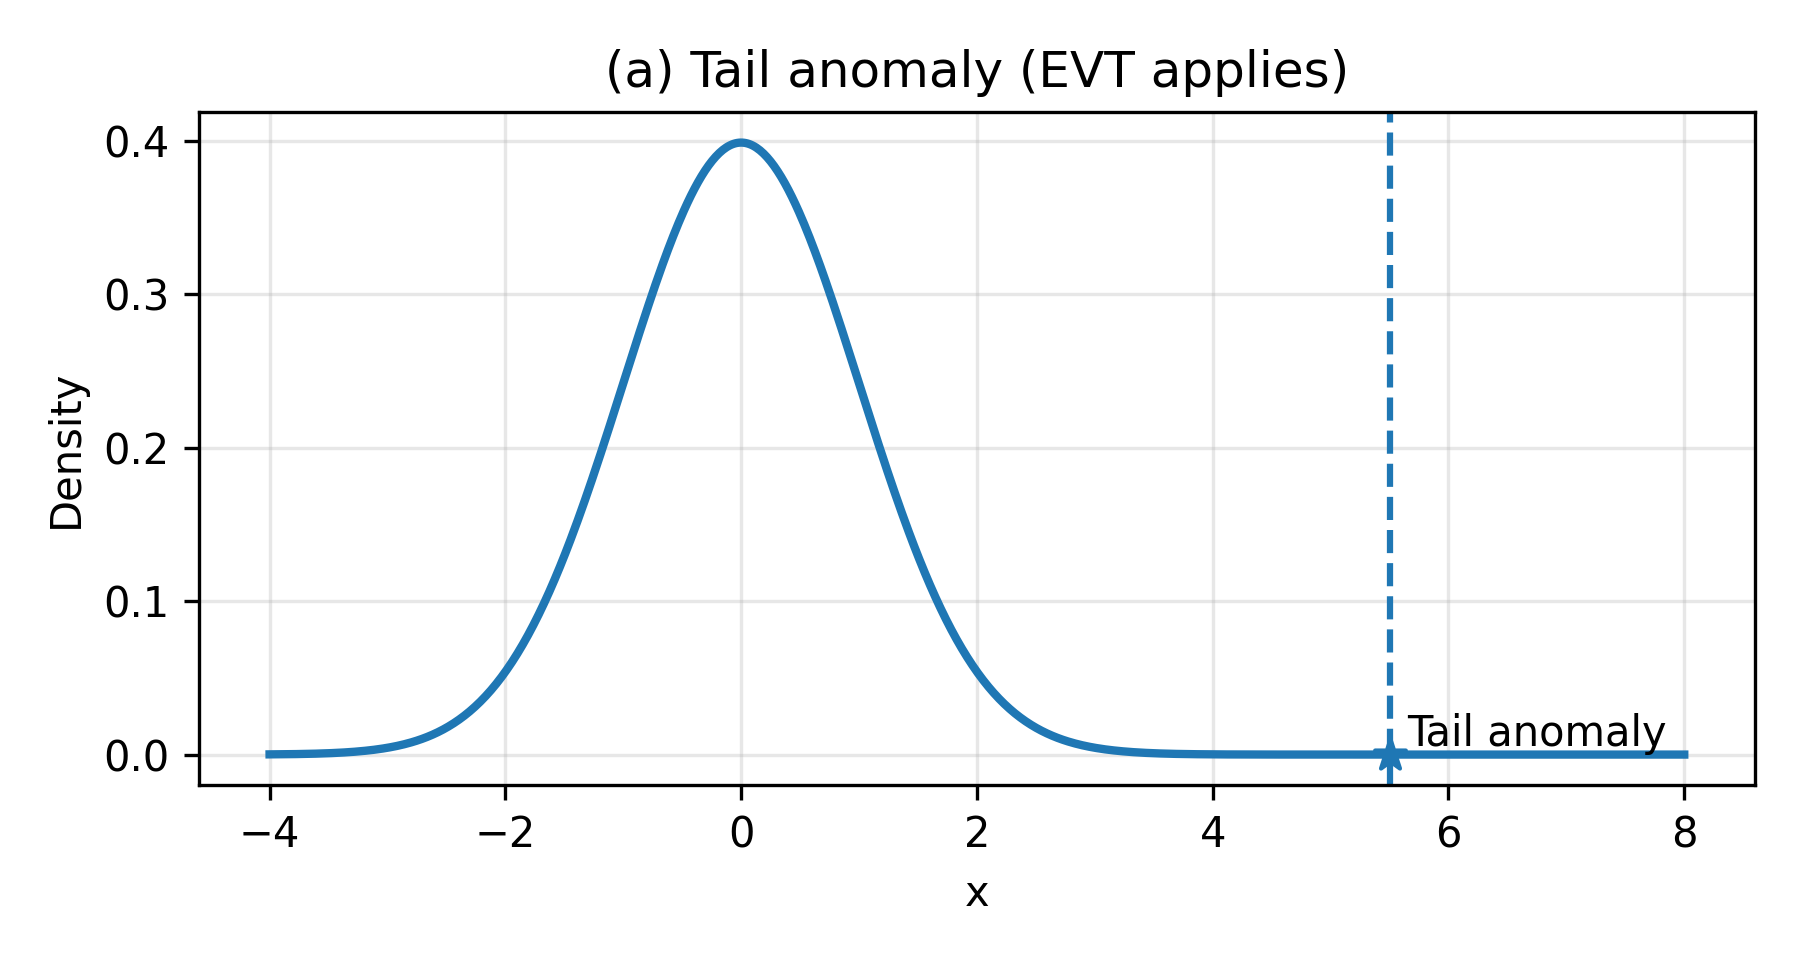
\includegraphics[width=\linewidth]{../output/others/evt_tail_anomaly.png}
    \vspace{0.25em}
  \end{minipage}\hfill
  \begin{minipage}{0.48\linewidth}
    \centering
    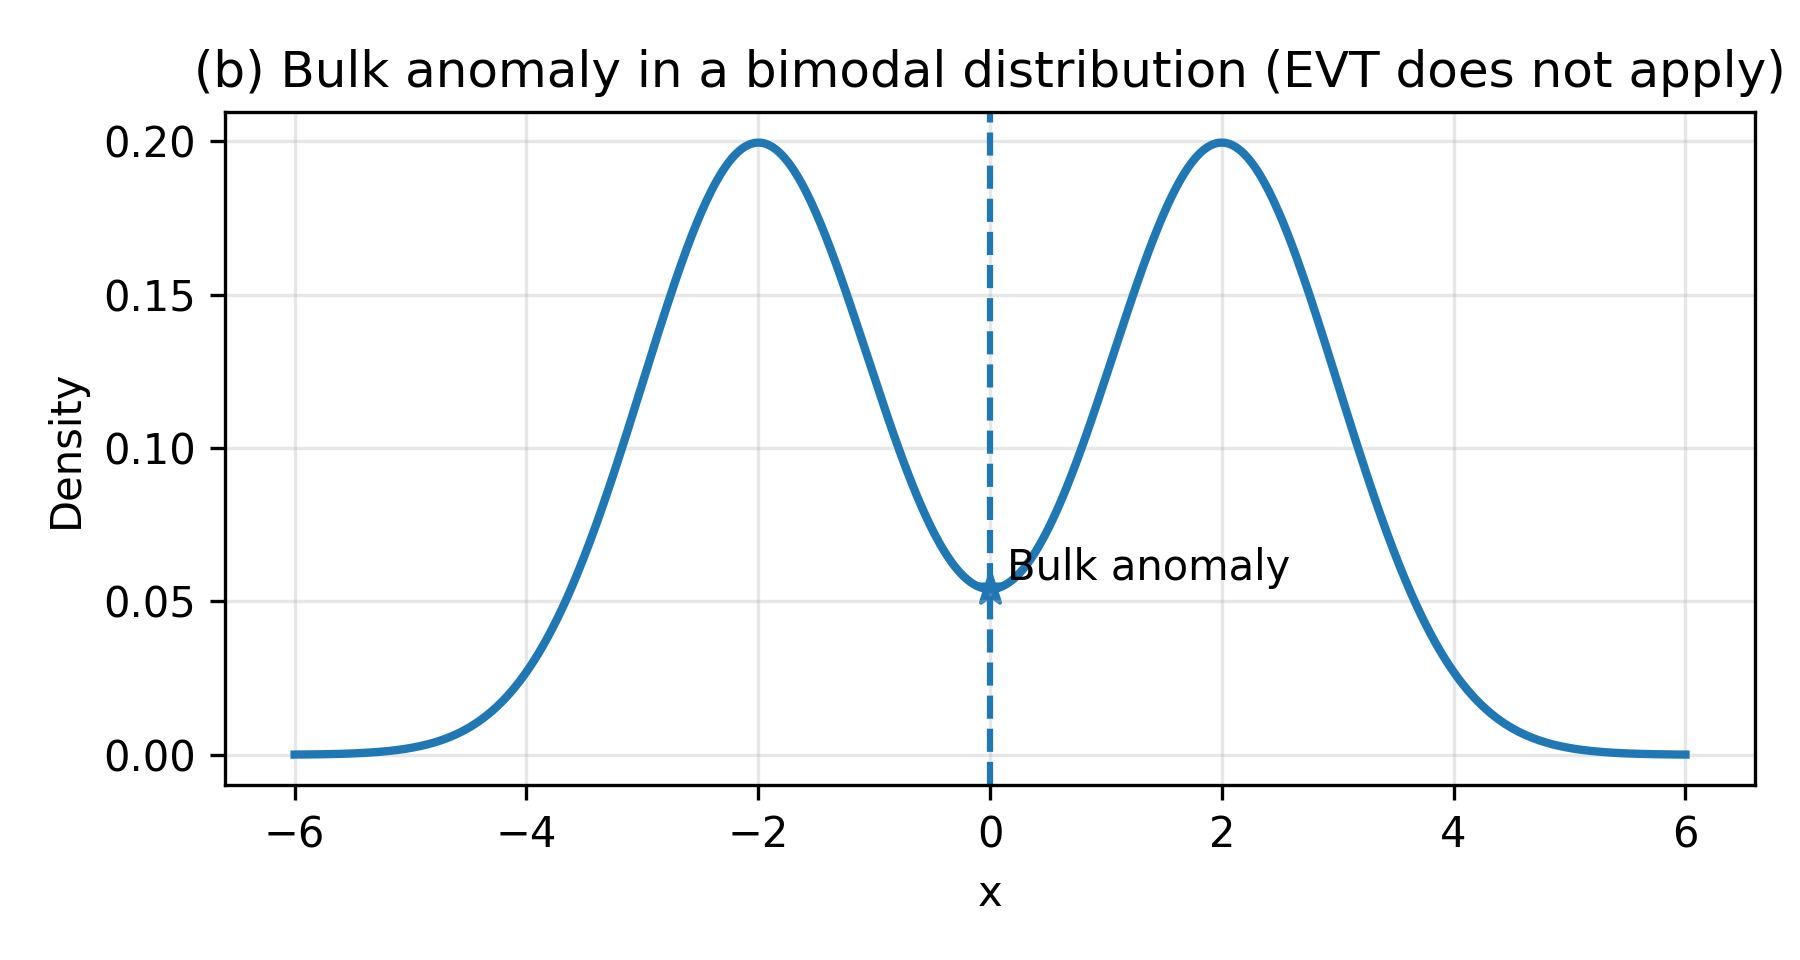
\includegraphics[width=\linewidth]{../output/others/evt_bulk_anomaly.png}
    \vspace{0.25em}
  \end{minipage}
  \caption{Illustrative anomalies relative to EVT. Concept suggested by Zak Varty (personal communication, 2025).}
  \label{fig:evt-anomalies}
\end{figure}

\subsubsection{Fisher-Tippett-Gnedenko Theorem (GEV)}

The Fisher–Tippett–Gnedenko theorem establishes that, under mild conditions, 
the distribution of suitably normalised block maxima converges to a member of the 
Generalised Extreme Value (GEV) family. In other words, regardless of the 
original distribution of the data, the extreme block maxima can be modelled by one of 
three limiting forms (Gumbel, Fréchet, or Weibull), unified by the GEV distribution 
parameterised by location, scale, and shape \citep{gnedenko1943distribution}. 

This result highlights the distribution-agnostic character of EVT: 
it guarantees that the statistical behaviour of extremes can be captured by a common 
family of models, making EVT widely applicable in anomaly detection tasks where 
the tail behaviour, rather than the full distribution, is of interest.
A formal statement of the Fisher–Tippett–Gnedenko theorem is provided in Supplementary 
Material~\ref{subsec:theorem_gev}.

\subsubsection{Pickands–Balkema–de Haan Theorem (GPD)}\label{subsec:gpd}

\begin{theorem}[Pickands–Balkema–de Haan] \label{thm:gpd}
Given a sufficiently high threshold \( u \), the distribution of exceedances 
\( Y = X - u \mid X > u \) converges to the 
\textbf{Generalised Pareto Distribution (GPD)}:
\begin{equation}
\mathbb{P}(X - u \le y \mid X > u) \approx G_{\gamma, \sigma_u}(y),
\label{eqn:gpd}
\end{equation}
with the GPD defined as
\begin{equation}
G_{\gamma, \sigma_u}(y) = 
\begin{cases}
1 - \left(1 + \gamma \tfrac{y}{\sigma_u} \right)^{-1/\gamma}, & \gamma \ne 0, \\
1 - \exp\!\left(-\tfrac{y}{\sigma_u}\right), & \gamma = 0,
\end{cases}
\quad y \ge 0, \; 1 + \gamma \tfrac{y}{\sigma_u} > 0,
\label{eqn:gpd-def}
\end{equation}
where \( \sigma_u > 0 \) and \( \gamma \in \mathbb{R} \).
\end{theorem}

\textbf{Theorem \ref{thm:gpd}} forms the foundation of the \textbf{Peaks Over Threshold (POT)} 
method, which involves modelling the distribution of threshold exceedances using the GPD 
\citep{balkema1974residual, pickands1975statistical, leadbetter1983extremes} and provides the theoretical basis for 
anomaly detection via principled estimation of extreme quantiles. 
It also emphasises that EVT does not attempt to model the entire distribution, but only the behaviour of 
exceedances beyond \( u \). Although originally derived for continuous random variables, the POT method is also widely 
applied to large integer-valued data such as packet counts or traffic volumes. In these settings, the discreteness of
the support becomes negligible once attention is restricted to the tail, so the GPD remains an adequate approximation 
for exceedances \citep{Coles2001, embrechts1997modelling}.

\subsubsection{Quantile Estimation under GPD}\label{subsubsec:quantile_est}

Let \( N_u \) be the number of exceedances over threshold \( u \), out of \( n \) observations. 
Given an estimated GPD, a high quantile \( z_q \) satisfying \( \mathbb{P}(X > z_q) = q \) 
can be estimated as:
\[
z_q \approx u + \frac{\hat{\sigma_u}}{\hat{\gamma}} 
\left( \left( \frac{N_u}{n q} \right)^{\hat{\gamma}} - 1 \right), \quad \hat{\gamma} \ne 0.
\]
as given in \citet{Coles2001,embrechts1997modelling}.

In POT-based anomaly detection, setting a \( q \) allows for direct control of 
how often false alarms occur, while the corresponding threshold \( z_q \) serves as a principled, 
interpretable detection rule. 

EVT, although theoretically rigorous, rests on a number of assumptions that limit its use in practice. 
One important requirement is that the exceedances behave roughly as independent observations. In reality
some dependence is tolerated, but only at short range; this is often expressed through mixing conditions 
such as Leadbetter’s \(D(u_n)\) criterion, which ensure that exceedances separated by enough time are 
close to independent \citep{leadbetter1983extremes,embrechts1997modelling}. Another difficulty lies in the
choice of the threshold \(u\). When \(u\) is set too high, only a few exceedances remain and estimates become
unstable. When it is set too low, points from the bulk of the distribution leak in and bias the fit 
\citep{Coles2001,embrechts1997modelling}. 

These conditions are easily violated in most real world streaming applications; 
the presence of autocorrelation, regime shifts, or evolving system dynamics undermines 
the reliability of POT-based methods. Addressing these limitations for non-stationary data 
is the central focus of this thesis.

\subsection{POT for Streaming Anomaly Detection}

Classical POT methods work well on static, stationary data, for which the discussed assumptions hold; 
however, real streaming data from open, dynamic environments often violates these assumptions. 
Consequently, researchers have developed streaming POT algorithms to adapt threshold 
models online. Notably, \citet{{siffer2017anomaly}} introduced the SPOT and DSPOT algorithms that 
adjust anomaly thresholds in real time, requiring only a user-specified risk level \( q \) 
(i.e. the desired false positive alarm rate) instead of a fixed threshold.

\subsubsection{SPOT (Streaming Peaks-Over-Threshold)}

SPOT sequentially updates an extreme-value threshold to flag anomalies in a univariate stream 
without assuming a fixed data distribution. First, an initial calibration batch of size \( n \)  is used 
to fit a GPD model and set two thresholds: an initial threshold \( t \) and an “alarm” threshold 
\( z_q\) corresponding to the desired risk level \( q \) , with \( z_q > t \). Once calibrated, 
each new observation \( X_i \) is classified into one of three cases: 
\begin{enumerate}
    \item \textbf{Normal:} if \( X_i < t \), the point is considered within the typical range.
    \item \textbf{Peak (Extreme but not anomalous):} if \( t \leq X_i < z_q \), the point is an extreme event; it is used to update the GPD model, but is not flagged as an anomaly.
    \item \textbf{Anomaly:} if \( X_i \geq z_q \), the point is flagged as anomalous; it is \emph{not} used to update the GPD.
\end{enumerate}

SPOT has three key hyperparameters: the calibration batch size \( n \), 
the risk level \( q \), and the initial threshold \( t \). 
\citet{siffer2017anomaly} report that the method is relatively robust to these choices. 
The initial batch size \( n \) mainly provides a starting estimate and, 
since we refit GPD as new peaks come in, does not significantly affect the long-term results. 
The authors also report that the risk parameter \( q \), which directly specifies the target false-alarm rate, 
can be chosen within a broad range (e.g., \( 10^{-5} \) to \( 10^{-3} \)) without dramatic changes 
in performance; in practice, \( q \) is set to match application requirements. 
Finally, for the initial threshold \( t \), the authors fix its value at the 98th empirical 
percentile of the calibration data. Although several EVT-based diagnostics exist for threshold selection, a 
common approach is to examine the \emph{stability of exceedances}--that is, to check whether estimated GPD 
parameters remain approximately constant as the threshold increases \citep{Coles2001,beirlant2004statistics}. 
In contrast, \citet{siffer2017anomaly} fix the initial threshold at the 98th empirical percentile, 
which was found to yield more consistent results in streaming settings.

\subsubsection{DSPOT (Drift Streaming POT)}\label{subsec:dspot}

To release the stationarity assumption, 
DSPOT incorporates a drift correction through a preprocessing step that aims to 
transform the input series into approximately stationary residuals. 
Specifically, each new value \( X_i \) is transformed as follows:

\[
X_i' = X_i - M_i
\]
where \( M_i \) is the \emph{local mean} of the most recent \(d\) non-anomalous observations:
\[
M_i = \frac{1}{d}\sum_{j \in \mathcal{H}_i^{(d)}} X_j, 
\]
with \(\mathcal{H}_i^{(d)}\) denoting the index set of the last \(d\) non-anomalous points before time \(i\),
with \(d\) referred to as the \emph{depth parameter} in \citet{siffer2017anomaly}. 
This centres the series around a local zero mean, ensuring that the residuals \(X'_i\) more closely 
satisfy the assumptions required by EVT tail modelling.

The depth parameter \( d \) determines how many past values are used to compute the local mean. If \( d \) is 
chosen too small, the estimate reacts quickly to changes in level but is also very noisy. If \( d \) is too large,
the mean becomes smoother, yet it can fail to keep up with genuine shifts in the series. In DSPOT, \citet{siffer2017anomaly}
treat \( d \) as a user-defined parameter and select it empirically in their experiments, rather than deriving it from 
theory. Although the exclusion of anomalous points stabilises the estimate, the choice of \( d \) still affects how well 
the method adapts to changes such as slow trends, abrupt shifts, or recurring seasonal patterns. 

Beyond the choice of \(d\), another key design decision in DSPOT is how the local mean \(M_i\) itself is defined. 
The original authors chose a simple moving average for \( M_i \) as a practical way 
to account for slow-moving drift. While effective in their tests, such preprocessing 
may be overly simplistic for complex real world data. Many time series exhibit seasonality, 
abrupt level shifts, or non-linear trends that a plain moving average might not capture, 
leaving residuals \( X'_i \) still non-stationary. 

This work extends the DSPOT framework by experimenting with alternative forms of preprocessing designed 
to deal with non-stationarity beyond slow drift. By doing so, the POT principle is retained, but its underlying
stationarity requirements are better met in practice.

\section{Methodology}\label{sec:methods}

\subsection{Alternative Preprocessing Pipeline}\label{subsec:alternative_pipeline}

As discussed in Section~\ref{subsubsec:quantile_est}, real world time series often violate the assumptions of 
standard extreme-value models. The standard guidance of how to address this is to 
either (i) model these effects explicitly via covariates or time-varying parameters, 
or (ii) pre-transform the data to yield an approximately stationary residual series 
\citep{Coles2001,DavisonSmith1990}. 

Since we are focusing solely on the streaming context, 
where data must be processed online with minimal delay, 
complex model-based non-stationary EVT approaches may be impractical in their standard batch form. 
Unlike the lightweight, local re-fitting used in SPOT/DSPOT, 
smooth non-stationary EVT models such as penalised-spline or covariate-based GPD parameterisations 
\citep{ChavezDemoulinDavison2005,NorthropJonathan2011} 
require retaining large historical datasets, repeated global optimisation over all exceedances, 
and tuning of smoothing parameters via information criteria or cross-validation. 
Such procedures are computationally intensive, memory-demanding, and therefore 
ill-suited for high-frequency streaming contexts where near-$O(1)$ processing 
is required, motivating our focus on alternative, fully online preprocessing techniques. 

In our work, we compare two preprocessing pipelines:
\textbf{(A) Moving-Average (MA) Detrending:} As a baseline, 
we implement a simple MA preprocessing as originally used in DSPOT.
Following the steps described in Section~\ref{subsec:dspot}, we aim to remove slow fluctuations 
and approximate the local expected value of the signal. The advantage of this approach is its simplicity, 
low computational cost and no strong assumptions about the form of the trend. 
However, its limitation is that it may be insufficient when the data has a 
strong periodic structure or changing variance. For the depth parameter \( d \), we do not treat it as a 
free tuning parameter. Instead, we set it in line with the dominant seasonal cycle of each dataset, 
so that the local mean captures recurring patterns while smoothing over short-lived fluctuations.

\textbf{(B) EWMA + Rolling Variance Normalisation + Seasonal Differencing:} 
As an alternative preprocessing pipeline, we introduce a more complex approach,
which we will hereafter refer to as the \emph{alternative preprocessing pipeline}. 
It consists of three steps as follows:

\emph{EWMA Trend Filtering:} 
We first remove long-term trends using an Exponentially Weighted Moving Average (EWMA),
a recursive filter defined by: 
\[
T_t = \alpha X_t + (1-\alpha)T_{t-1}
\]
where $T_t$ is the estimated trend, $0<\alpha<1$ is a smoothing factor and is initialised with $T_0=X_0$. 
We choose a small \( \alpha \) (in our implementation, $\alpha = 0.05$) 
so that the filter has a long memory, effectively capturing slow changes in the baseline level 
while smoothing out short-term fluctuations. We subtract this trend from the series to get a 
detrended value: $X_t' = X_t - T_t$. We prefer EWMA to a simple moving average here 
because its exponentially decaying memory provides smoother adaptation to gradual drift.

\emph{Rolling Z-Score Normalisation:} 
Next, we stabilise the scale and remove any residual local bias by standardising the 
detrended series $X_t'$ over a rolling window of length $P$, chosen to match the 
dominant seasonal period. Let $\bar{X}'_t$ and $s_t$ denote the sample mean 
and unbiased standard deviation 
(using dof = $1$ for an unbiased estimate) of the most recent $P$ values of $X_t'$. 
We compute the normalised value as:
\[
Z_t = \frac{X_t' - \bar{X}'_t}{s_t}.
\]
This step addresses heteroskedasticity by rescaling each observation relative to 
its local mean and variance, producing a dimensionless series whose short-term 
distribution is approximately $\mathcal{N}(0,1)$. This allows a constant EVT 
threshold to be applied in a meaningful way, independent of local variance changes. 
Choosing $P$ to coincide with the seasonal cycle ensures that the estimated mean 
and variance reflect a complete period of typical behaviour; the same $P$ is also 
reused in the next step. To prevent unreliable scaling and spurious extreme values, 
we impose a short warm-up period ($\ge 5$ points); 
during this stage, or whenever $s_t$ is numerically close to zero, no normalised 
value is emitted downstream.

\emph{Seasonal Differencing:} Finally, we remove repetitive cyclical patterns by subtracting 
the value from the previous period. 
For a chosen season length $P$, 
we compute a seasonal difference: 
\[ 
z_t^{(s)} = z_t - z_{t-P}
\]
Essentially, for each time $t$, we look one period back and remove that 
effect: $z_t^{(s)}$ should be near zero if the series at time $t$ behaves similarly
to time $t-P$. This cancels any additive seasonal effects that 
remain after detrending and normalisation. As with the earlier step, 
we suppress output during the initial warm-up period, until \( P \) past observations have been collected.. 
While seasonal differencing is a standard technique in time series 
analysis to achieve stationarity when strong periodicity is present, 
we note that this requires knowledge of the dominant period $P$; 
in our implementation, the same $P$ is leveraged both for rolling normalisation 
and for seasonal differencing.

This alternative preprocessing pipeline can be adapted to the characteristics of a given dataset: 
if the data exhibits no variance changes, the normalisation step can be skipped; 
if no clear periodicity exists, seasonal differencing can be omitted. 
By design, the pipeline aims to satisfy EVT’s assumptions as closely as possible, 
in line with the established practice of first transforming the data to produce 
(approximately) stationary residuals before tail modelling 
\citep{Mentaschi2016,EastoeTawn2009}. Lastly, the alternative pipeline is fully
suitable for real-time monitoring: all steps are computed incrementally, 
and the computational complexity is $O(1)$ per data point (constant-time updates of the EWMA, 
a subtraction for seasonal difference, and a fixed-size standard deviation computation). 

\subsection{Preprocessing Pipelines Comparison}\label{subsec:ppc}

Compared to the minimal MA baseline, the alternative preprocessing pipeline may offer advantages in 
non-stationary scenarios, particularly when the data exhibit time-varying variance or recurring 
seasonal patterns, since it addresses these alongside slow drift in the mean.
By stabilising both the mean and variance, and by removing predictable periodic structure, 
the resulting residual process should more closely satisfy the approximate independence and 
stationarity conditions underpinning the theoretical justification of GPD modelling. 
Moreover, the enhanced structure of the alternative pipeline should reduce
inflated false positives by preventing over-reaction to normal 
daily peaks or bursts of higher variance, and reduce false negatives by enabling the 
detection of anomalies even during low-variance periods. In Section~\ref{subsec:evt_diagnostic}, 
we will compare the two pipelines to quantify the gains from 
enforcing stationarity, thereby assessing whether the added complexity of the richer approach 
is justified. 

Since the asymptotic justification for POT via Theorem~\ref{thm:gpd} requires the underlying process to be stationary
and at most weakly dependent (see Section~\ref{subsubsec:quantile_est}), it is natural to check whether the exceedance
process and corresponding excess distribution are consistent with these conditions. In practice, the bulk of the series
(i.e. the non-extreme observations below the chosen threshold) does not need to behave as an i.i.d. sample; what matters
is that, above a sufficiently high threshold, exceedances occur in a way that is close to independent and that their 
distribution can be stabilised. If this is the case, POT remains valid even when the body of the series shows dependence
or other departures from i.i.d. behaviour. Problems arise, however, when non-stationarity or serial correlation in the 
bulk propagate into the tail, since this can lead to threshold instability or clusters of exceedances that distort inference
\citep{leadbetter1983extremes,embrechts1997modelling,resnick2007heavy}. For this reason, our primary diagnostics focus on 
the exceedance process itself, but we also report supporting checks on the full series. Together these assessments allow
us to judge whether the data are compatible with the weak-dependence assumptions needed for tail modelling, and whether 
a GPD fit provides an adequate description of the excess distribution. To do so, we use the following framework.

First, linear and nonlinear independence of the full series is assessed.We use three complementary tools. 
(i) \emph{Autocorrelation function (ACF):} the ACF at lag $k$ estimates 
$\rho(k)=\mathrm{Corr}(X_t,X_{t-k})$ \citep{brockwelldavis1991}. 
Under independence, $\rho(k)\approx 0$ for small $k$; empirically, sample ACF ordinates should lie within 
approximate 95\% bounds ($\pm 1.96/\sqrt{n}$) for moderate lags. Visual confinement within these bands supports 
the no linear dependence assumption. 
(ii) \emph{Ljung--Box portmanteau test} \citep{ljung1978measure}: for a chosen cutoff $m$, 
the statistic $Q(m)$ jointly tests $H_0:\rho(1)=\cdots=\rho(m)=0$. It may be viewed as a quantitative complement 
to the ACF plot. A large $p$-value (failure to reject $H_0$) indicates no evidence of linear autocorrelation 
up to lag $m$. 
(iii) \emph{Brock--Dechert--Scheinkman (BDS) test} \citep{brock1996test}: this is a global test of 
$H_0$ that the series is i.i.d., based on differences in correlation integrals across embedding 
dimensions $m\ge 2$ with a neighbourhood size $\epsilon$. A large $p$-value (non-rejection) across sensible 
$(m,\epsilon)$ choices supports the i.i.d.\ assumption. Because the null hypothesis bundles independence together with 
constancy of the marginal distribution, rejection may arise from serial dependence, unremoved 
non-stationarity, or both. We therefore interpret BDS results jointly with the ACF/Ljung--Box and the 
tail-fit diagnostics.

Second, exceedance-process independence is examined. 
We repeat ACF, Ljung--Box, and BDS on the exceedance series alone, defined relative to the empirical 
$98^\mathrm{th}$ percentile. Significant autocorrelation or BDS rejection at this stage would suggest 
dependence or non-stationarity among exceedances, of which \emph{extremal clustering}---the tendency of 
extremes to occur in bursts---is the primary concern \citep{leadbetter1983extremes}. 
Ideally, exceedances should occur approximately independently in time, without evidence of serial dependence.

Third, tail-model adequacy is evaluated.
Excesses over the chosen threshold are fitted to a GPD with location fixed at zero, 
and the fit is assessed via \emph{quantile--quantile (Q--Q) plots}, which compare empirical quantiles of excesses 
to theoretical GPD quantiles \citep{Coles2001}, and a \emph{Kolmogorov--Smirnov (KS) goodness-of-fit test}, which 
is viewed as a quantitative complement to the Q--Q plot.\citep{massey1951kolmogorov}. 
The KS test compares the empirical CDF of excesses to the fitted GPD CDF under $H_0$: excesses follow the specified GPD. 
A large $p$-value (i.e. failure to reject) indicates no detectable discrepancy, while systematic curvature 
in the Q--Q plot or a small $p$-value signals model misspecification, residual non-stationarity in the tail, 
or a threshold set too low to isolate genuine extreme behaviour.

\subsection{EQD-Enhanced Threshold Selection}\label{subsec:eqd}

Thus far, our methodology has focused on mitigating non-stationarity in streaming data via preprocessing. 
A complementary challenge in POT-based anomaly detection is the selection of 
the initial threshold for tail modelling. In the original SPOT and DSPOT algorithms, 
this threshold $t$ is set heuristically: \citet{siffer2017anomaly} simply chose $t$ as the 98th percentile of 
an initial batch to ensure it is \emph{high enough} to provide a valid GPD approximation of exceedances. 
While this pragmatic choice worked reasonably well in their tests, 
it is not guaranteed to be optimal for all datasets. 
Threshold selection is well known to be a critical and non-trivial problem in extreme value analysis 
\citep{Coles2001,DavisonSmith1990}. An inappropriate choice can skew the entire detection procedure: 
setting $t$ too low violates the asymptotic assumptions of the GPD and biases the tail fit (yielding too many false alarms), 
while setting $t$ too high results in too few exceedances and unstable estimates (yielding missed anomalies). 
This represents the classic bias--variance trade-off \citep{NorthropJonathan2011}, and inference is highly sensitive to it. 
Although \citet{siffer2017anomaly} acknowledged the issue, they did not pursue principled methods for threshold selection. 
To strengthen the robustness of our streaming POT approach, 
we incorporate an automated threshold selection procedure into SPOT's/DSPOT’s initialisation, rather than relying on a fixed quantile. 

We adopt the Expected Quantile Discrepancy (EQD) criterion recently proposed by \citet{murphy2025eqd}, 
which builds on earlier diagnostic ideas introduced by \citet{varty2021earthquake}. 
Designed to optimise threshold choice by explicitly balancing bias and variance, 
the EQD method provides a quantitative measure of how well a GPD model fits the tail for a given threshold, 
averaged across bootstrap resamples. In essence, it operates as follows. 
We consider a grid of high threshold candidates (in our implementation, the 90th to 99.5th percentiles of the calibration data). 
For each candidate threshold $u$, we fit a GPD to the excesses above $u$ in the initial batch. 
We then generate many bootstrap samples (with replacement) of these excesses and, for each, 
compute the mean absolute deviation between empirical quantiles and those predicted by the fitted GPD,
averaged over a grid of \(m=500\) quantile levels. By averaging these deviations over \(B\) resamples, 
we obtain the \emph{expected quantile discrepancy} $D(u)$ for threshold $u$. 
The optimal threshold $u^*$ is then chosen as the minimiser of $D(u)$. 
In effect, $u^*$ is the point at which the GPD provides the most reliable fit, 
balancing the bias of including too many non-extremes against the variance of fitting too few exceedances.

The EQD criterion offers several advantages over commonly used threshold selection approaches, 
including heuristic quantile rules (e.g.\ fixing the threshold at the 98th percentile), 
graphical diagnostics based on mean residual life or parameter stability plots, 
and goodness-of-fit tests such as Kolmogorov--Smirnov p-values\citep{Coles2001,DavisonSmith1990}.
Unlike these methods, which are either arbitrary or unstable with limited data \citep{NorthropJonathan2011}, 
EQD provides a principled and reproducible criterion grounded in model fit. 
By averaging discrepancies across bootstrap resamples, it smooths out the randomness that 
hampers p-value-based and graphical methods, and yields a transparent and objective optimum. 
Simulation studies by \citet{murphy2025eqd} further demonstrate that EQD-based thresholds produce
more accurate extreme quantile estimates than competing automated methods, 
while remaining robust to tuning choices such as the number of bootstrap replicates $B$. 
Very small calibration samples can also destabilise EQD, as bootstrap resamples of only a handful of exceedances yield 
highly variable estimates. However, in very small calibration samples, the limited number of exceedances may result in 
sparsely populated bootstrap resamples, leading to unstable EQD estimates and erratic threshold selection.

\paragraph{Integration into DSPOT.} 
We implement EQD during the offline calibration phase of DSPOT. 
After preprocessing the initial calibration window using one of our pipelines, 
the resulting residuals are treated as approximately i.i.d. data for threshold analysis. 
Each candidate threshold is then fitted via the Grimshaw maximum likelihood algorithm for the GPD 
\citep{grimshaw1993computing}, and the EQD metric is estimated using $B=100$ bootstrap replicates. 
The choice of $B=100$ follows the recommendations of \citet{murphy2025eqd}, who found this setting to 
provide stable estimates at modest computational cost. To avoid instability when only a handful of exceedances are available, 
we further required at least ten exceedances above any candidate threshold, thereby ensuring that 
the $D(u)$ curve remained stable and interpretable. The most promising threshold typically emerges 
as a clear minimum in the $D(u)$ curve: lower thresholds suffer bias-induced misfit, 
whereas extremely high thresholds show erratic behaviour due to sampling variability. 
Once the optimal threshold $u^*$ is identified, we refit the GPD on all exceedances above $u^*$ 
and compute the corresponding alarm threshold $z_q$ for the desired false alarm rate $q$. 
This data-adaptive selection replaces the fixed 98th percentile rule used in the original DSPOT. 
Importantly, the EQD procedure does not alter the subsequent online detection phase: 
it is a one-time enhancement confined to initialisation, with modest computational cost 
(on the order of seconds for $n \approx 1000$). Once streaming begins, DSPOT proceeds as usual with $O(1)$ updates per point.

Nevertheless, the method rests on certain preconditions. It assumes the calibration data is approximately 
i.i.d.\ and stationary in the upper tail. Our preprocessing steps aim to satisfy this, but temporal dependence, 
such as the clustering of extremes, may still persist in the tail and could mislead the criterion if not accounted for. 
Besides, if the calibration window contains transient anomalies (e.g. one-off spikes or bursts that are true anomalies 
rather than \emph{normal extremes}), the chosen threshold may be distorted. Finally, while DSPOT's online updating can 
correct moderate model misspecification, substantial non-stationarity shortly after initialisation 
may render the initially calibrated threshold less useful. 
In such environments, periodic re-calibration could be considered.

In summary, EQD-based initialisation enhances POT-based anomaly detection by automating a key step that was left heuristic 
in the original design. When applied to reasonably sized, approximately stationary calibration data, 
it should provide a principled threshold that improves the calibration of alarm rates, 
reducing both false positives and false negatives. In highly volatile environments with very limited calibration data, 
however, its advantages may diminish. This trade-off mirrors the broader theme of our work: robustifying POT-based detection 
by addressing both non-stationarity (through preprocessing) and threshold selection (through EQD).

\section{Application to Cannonical Datasets}\label{sec:res}

\subsection{Datasets}\label{subsec:my_subsec}

We will evaluate POT-based anomaly detection methods using three real world time series datasets sourced from the 
Numenta Anomaly Benchmark (NAB) repository \citep{lavin2015evaluating}. 
The NAB framework is a widely used benchmark for streaming anomaly detection, providing publicly available time series 
with ground truth anomaly labels across a variety of domains. The raw series are shown in 
Figure~\ref{fig:raw_datasets}, and a detailed description of each dataset is provided below.

\begin{enumerate}
    \item \textbf{CPU Utilisation (AWS EC2 Server):} 
    This dataset records the CPU usage (\%) of an Amazon EC2 instance at 5-minute intervals. 
    The series displays a long, stable baseline with small stochastic fluctuations and occasional sharp spikes, 
    typically lasting only one or two samples, reflecting short-lived workload bursts. 
    The series exhibits two downward level shifts: a smaller one around 18 February and a more pronounced one 
    around 24 February, after which the baseline stabilises at a lower mean.
    Thus, the process can be regarded as piecewise stationary with respect to the mean, 
    while the variance remains approximately constant. No strong daily periodicity is evident. 
    In principle, a simple MA detrending procedure would be sufficient. However, we will deliberately apply the full 
    alternative pipeline here, both to assess its behaviour on a relatively simple series and to illustrate how unnecessary
    preprocessing may distort the statistical properties of otherwise well-behaved data.
    In this sense, the CPU data illustrate the risk of overprocessing: unless preprocessing is aligned with the underlying
    structure, it can introduce distortions instead of improving model validity (Figure~\ref{fig:raw_datasets}a).
    \item \textbf{Twitter Volume (AMZN Hashtag):} 
    This dataset comprises 5-minute counts of tweets containing the ``AMZN'' hashtag. 
    The series shows an underlying daily periodicity. Superimposed on this daily cycle are occasional extreme spikes, 
    often more than an order of magnitude above the baseline, driven by exogenous events such as news about Amazon 
    or major announcements. As seen in the differing heights of daily peaks across time, both the amplitude of the 
    daily cycle and the background variance fluctuate substantially; the result is a process that is strongly non-stationary 
    in both mean and variance. Anomalies are therefore defined relative to the evolving local baseline, rather than 
    simply as global maxima. The combination of daily seasonality, heteroskedasticity, and irregular extreme bursts 
    makes this dataset particularly challenging for POT-based anomaly detection, and motivates the use of the full 
    alternative preprocessing pipeline (Figure~\ref{fig:raw_datasets}b). Notably, this dataset is the only integer-valued
    one in our study. Following standard practice (see Section~\ref{subsec:gpd}), 
    we treat exceedances as approximately continuous, which is justified by the large scale of observed counts. 
    \item \textbf{Traffic Occupancy (Road Sensor 6005):} 
    This dataset consists of 5-minute readings of freeway lane occupancy, measured as the percentage of time a loop detector
    registers a vehicle. The series shows a strong daily cycle associated with morning and evening rush-hour traffic. The 
    heights of the daily peaks vary somewhat across days, and the single labelled anomaly corresponds to congestion levels
    that exceed the typical rush-hour maxima. The dataset also contains missing values, including a long contiguous gap; 
    for analysis, we restrict attention to a cleaned, continuous segment beginning on 11 September, thereby avoiding 
    distortions from the missing period. Because of its pronounced daily periodicity and moderate variation in peak intensity,
    the dataset provides a useful test case for seasonality removal and rolling variance normalisation
    (Figure~\ref{fig:raw_datasets}c).
\end{enumerate}

\begin{figure}[ht]
  \centering
  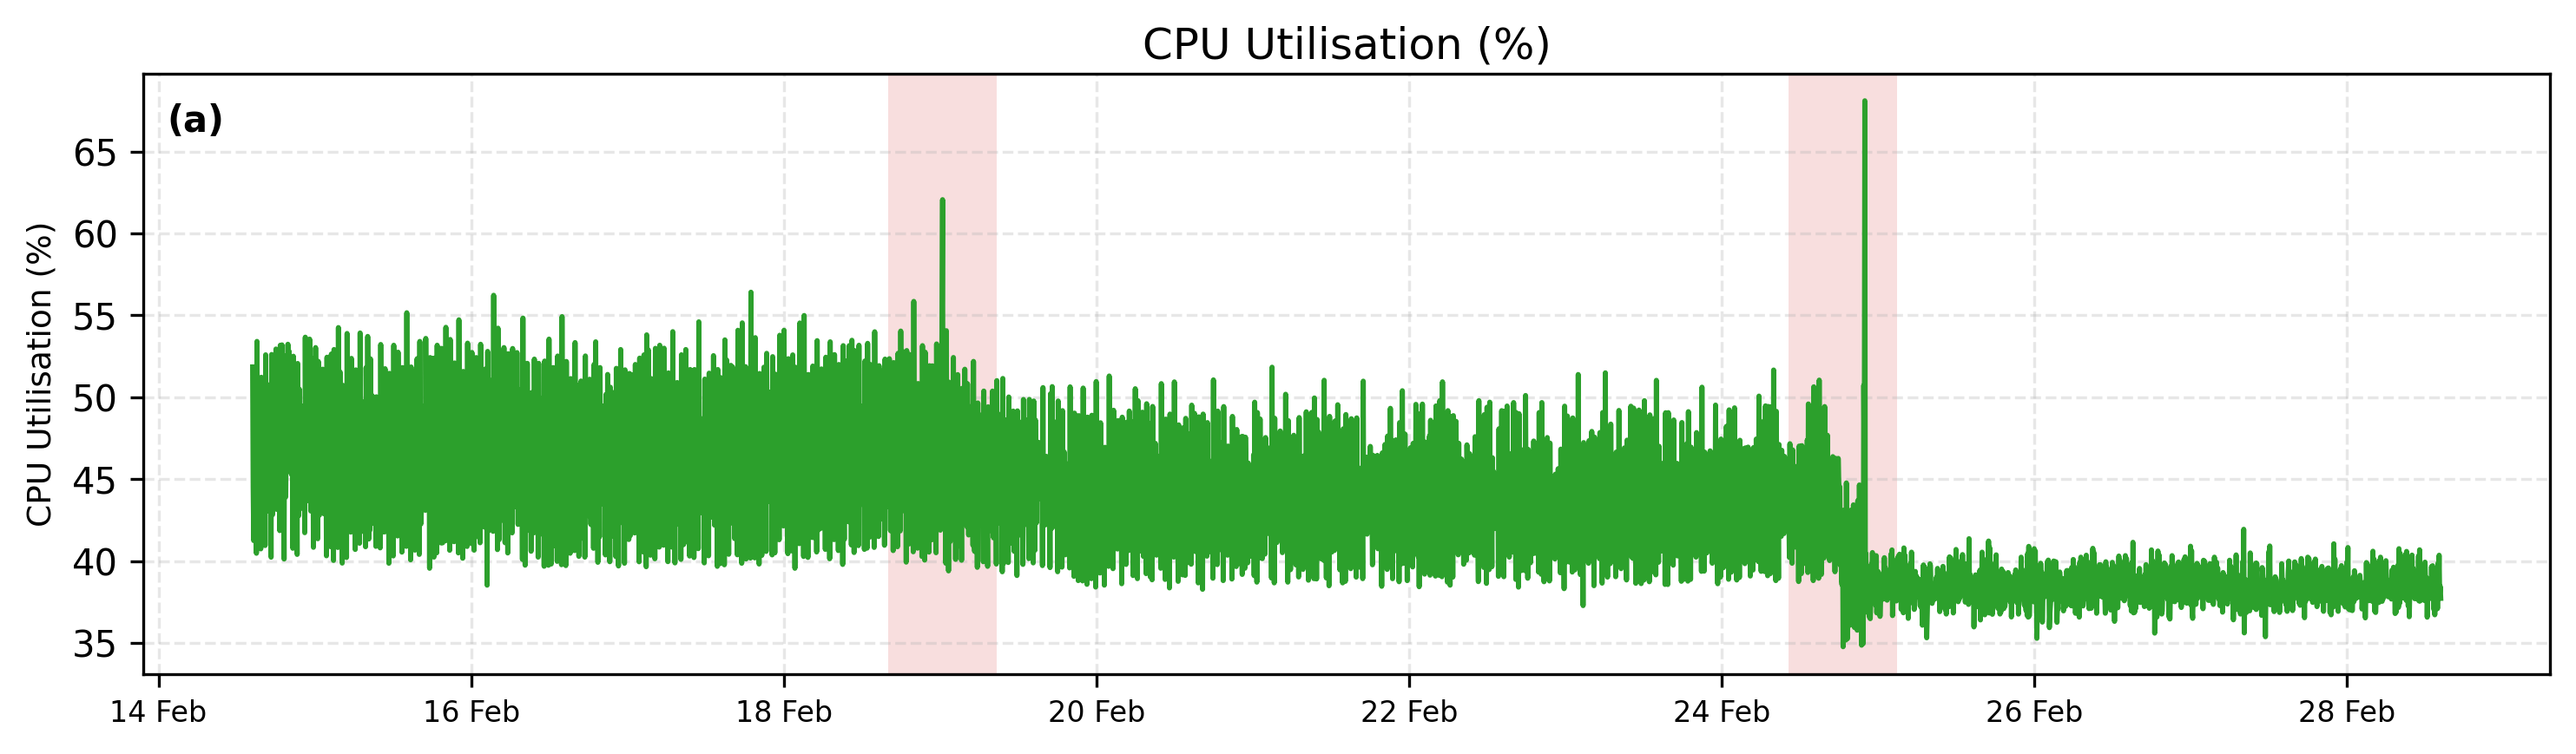
\includegraphics[width=\linewidth]{../output/cpu/cpu_raw_seris.png}\par\vspace{0.35em}
  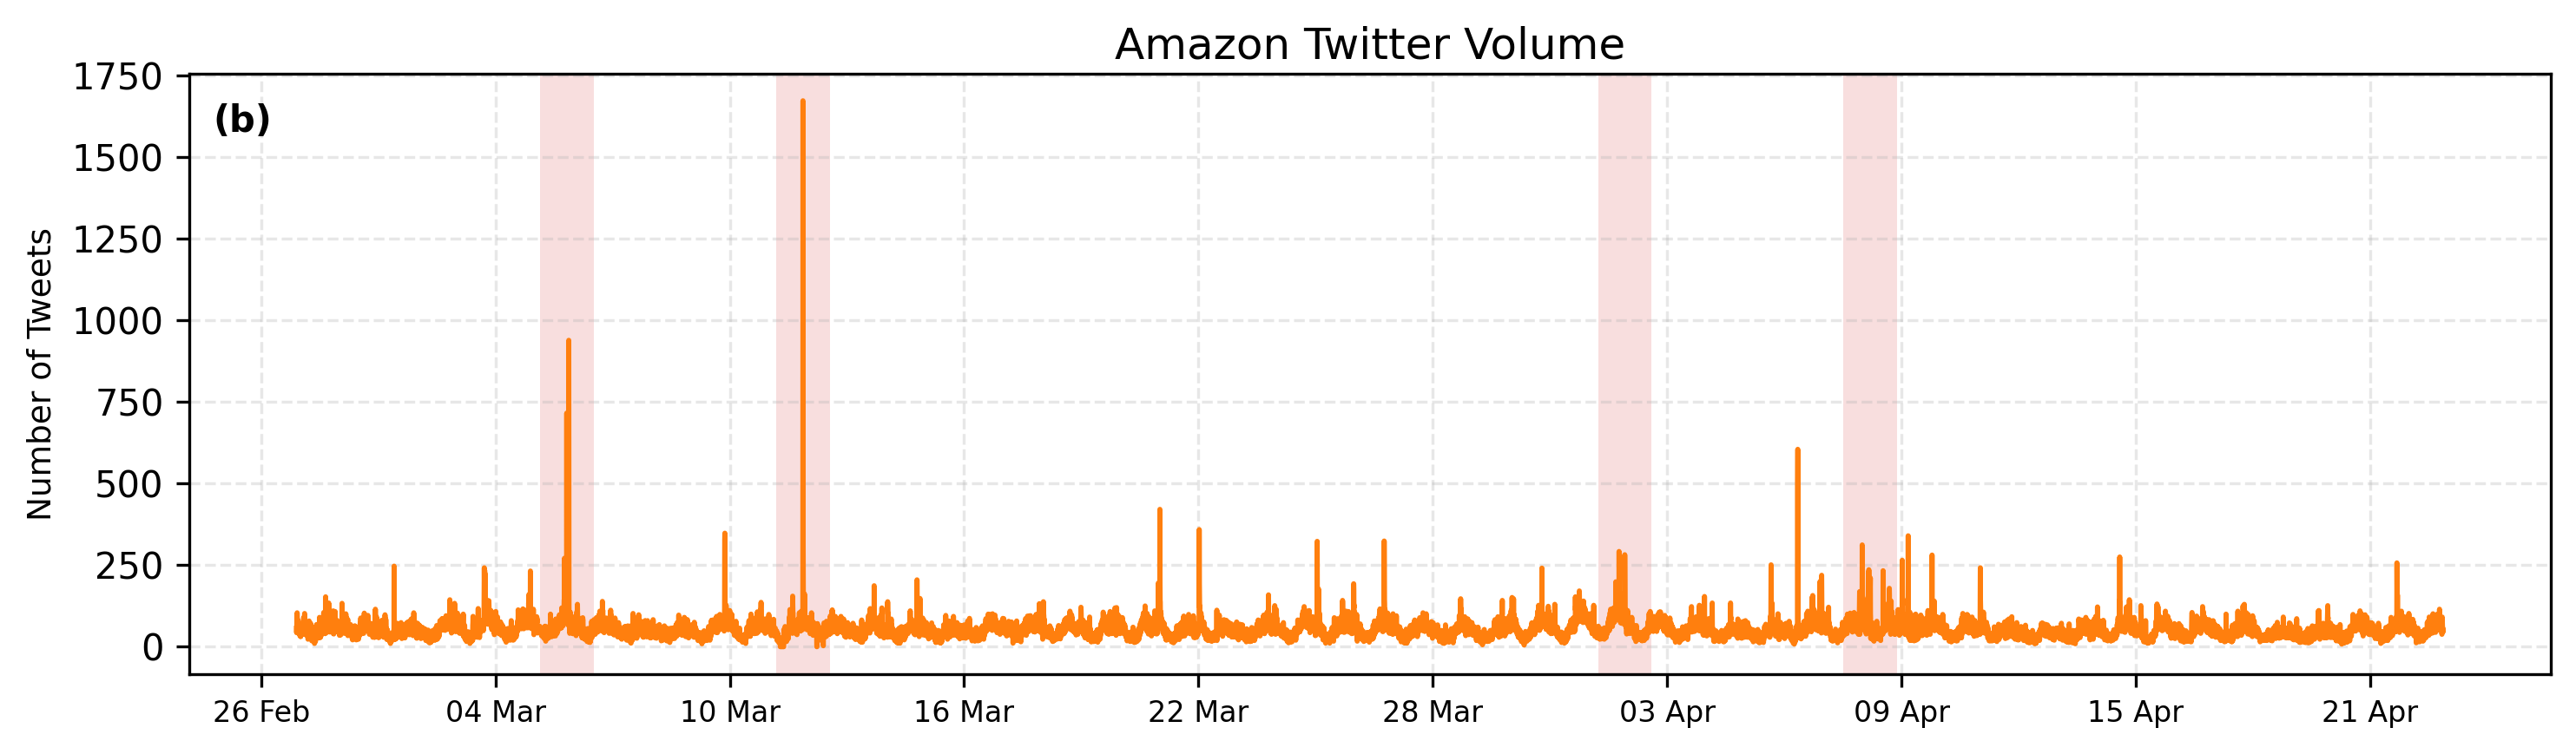
\includegraphics[width=\linewidth]{../output/realTweets/realTweets_raw_seris.png}\par\vspace{0.35em}
  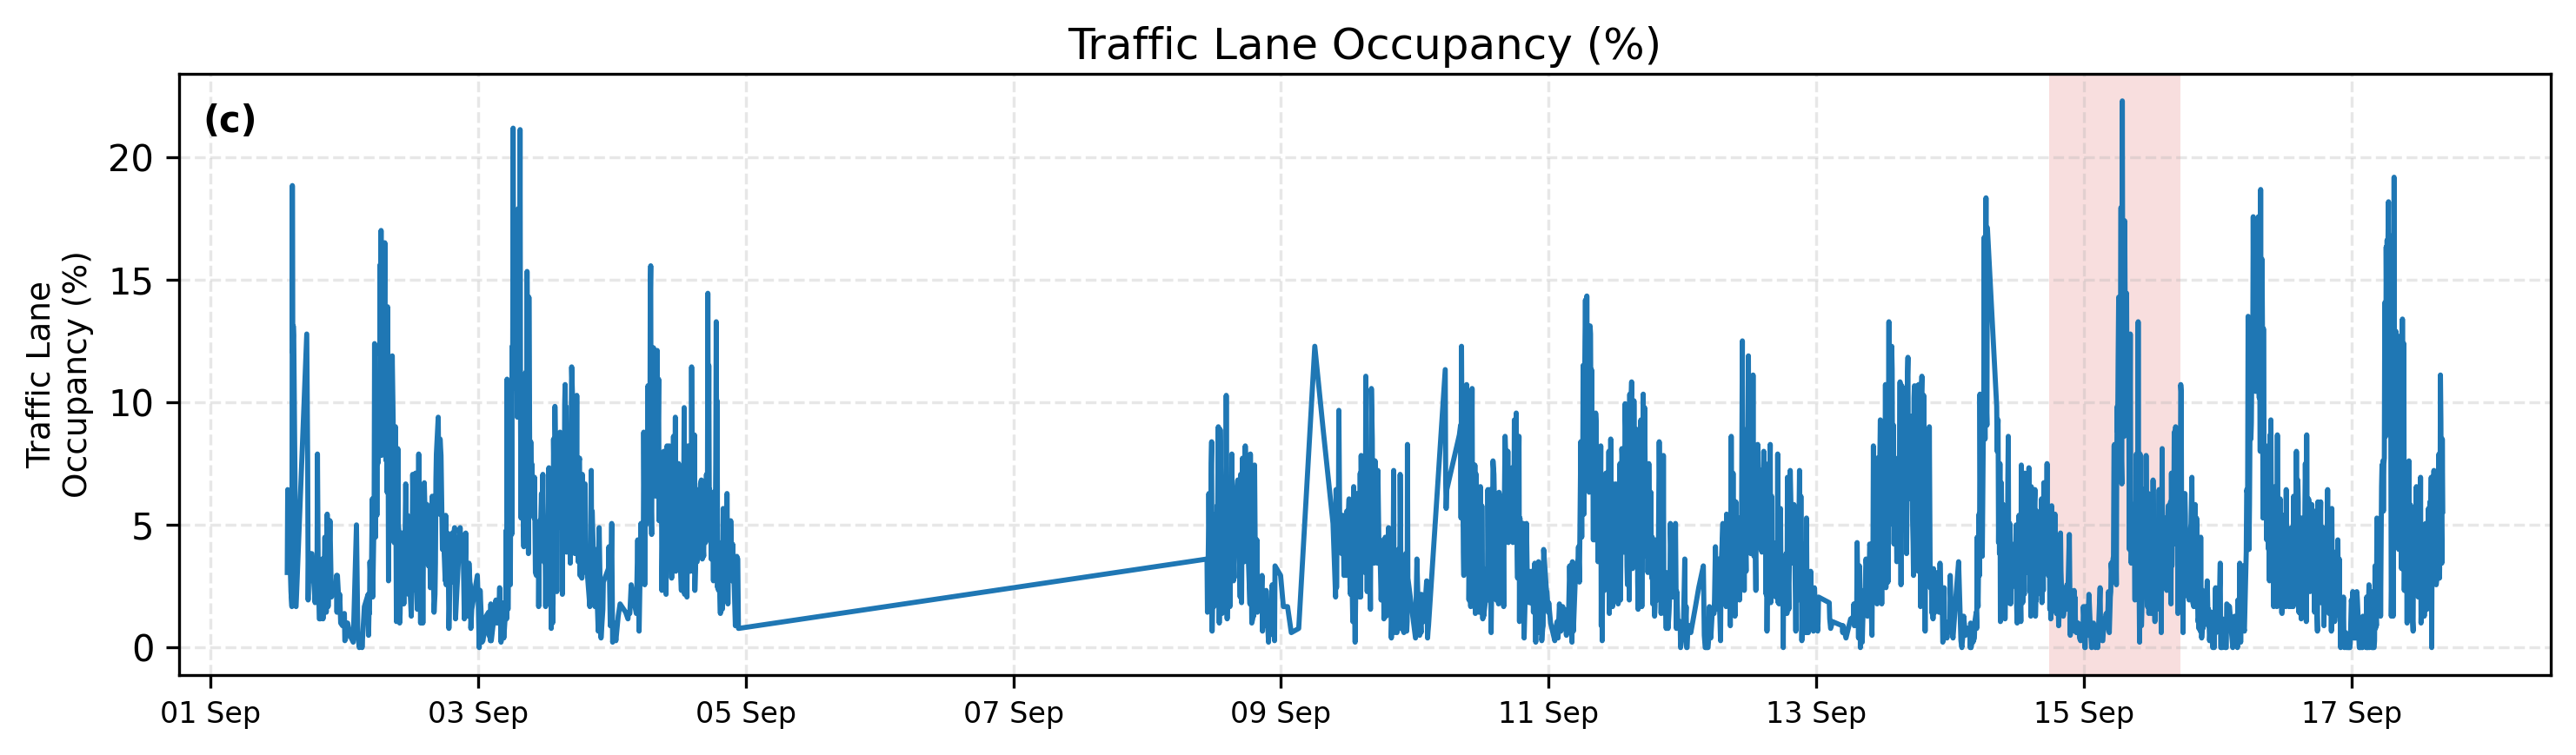
\includegraphics[width=\linewidth]{../output/occupancy/occupancy_raw_seris.png}
  \caption{Raw time series: (a) CPU Utilisation, (b) Amazon Twitter Volume 
  and (c) Traffic Occupancy. Each panel preserves the original timestamp scale; shaded red bands highlight ground-truth anomaly windows.}
  \label{fig:raw_datasets}
\end{figure}

Taken together, the three datasets exhibit complementary forms of non-stationarity: a mean shift without variance changes 
(CPU Utilisation), daily periodicity combined with heteroskedasticity (Twitter Volume), and strong seasonality with drifting 
variance (Traffic Occupancy). Their diversity provides a natural framework for assessing anomaly detection 
performance under non-stationary conditions, as outlined in the following evaluation strategy.

\subsection{Event-based Evaluation Protocol}\label{subsec:event_ev}

To assess the performance of the POT-based anomaly detection methods, 
we adopt an event-based evaluation, in which contiguous labelled anomaly windows constitute the unit of analysis.
Because anomalies in time series are often contiguous periods of abnormal behaviour (rather than single isolated points), 
event-based metrics are more meaningful than pointwise error rates \citep{lavin2015evaluating}. For counting purposes we collapse 
consecutive alarmed samples into a single alarm event; two alarm events are distinct only if separated by at 
least one non-alarm sample (i.e., a silent gap of one sampling interval), endpoints inclusive. 
We define the evaluation components as follows:

\begin{itemize}
    \item \textbf{True Positive (TP):} 
    A ground-truth anonaly window that was successfully detected by the algorithm. 
    We count an event as detected if at least one alarm was raised during the anomaly window’s duration. 
    Multiple alarms within the same window still count as one TP in event-based evaluation.
    If an alarm overlaps more than one anomaly window, it is credited only to the first unmatched window.
    
    \item \textbf{False Positive (FP):} 
    An alarm event that does not overlap any ground-truth anomaly window. 
    
    \item \textbf{False Negative (FN):} 
    A ground-truth anonaly window that the detector failed to catch (i.e., no alarm occurred within its duration).
\end{itemize}

Using these counts, we compute the standard metrics:
\begin{itemize}
    \item \textbf{Precision (P):}
    \( P = \dfrac{\text{TP}}{\text{TP} + \text{FP}} \). This is the proportion of raised alarm events 
    that correspond to ground-truth anomaly windows. 
    We report P as NA if \( \text{TP}+\text{FP}=0 \) (no alarms raised).

    \item \textbf{Recall (R):}
    \( R = \dfrac{\text{TP}}{\text{TP} + \text{FN}} \). This is the proportion of ground-truth anomaly windows
    that were detected. We report R as NA if \( \text{TP}+\text{FN}=0 \) 
    (no ground-truth anonaly windows).

    \item \textbf{F1-score:}
    \( \text{F1} = 2 \cdot \dfrac{P \cdot R}{P + R} \). The harmonic mean of precision and recall, which 
    provides a single balanced measure that accounts for both false alarms and missed detections.
    F1 is not reported (NA) when either \( P \) or \( R \) is undefined.

    \item \textbf{Detection Delay:}
    For each detected event (TP), the delay is the time (in minutes) from the event start to the timestamp of 
    the first alarm within that event. Undetected events are excluded from delay summaries.
\end{itemize}

To ensure fair comparison across methods and datasets, we fix the POT nominal tail risk level \(q\) identically in all runs 
(e.g., \( q = 10 ^{-3}\) ), so that differences in performance reflect preprocessing and updating rather than differing 
alarm thresholds. We therefore compare methods at a common operating point using event-based precision, recall, F1, 
and detection delay.

\paragraph{Uncertainty and small-sample reporting.}
Precision and recall are accompanied by 95\% Wilson score confidence intervals, treating each as a binomial proportion
(precision: x = successes \(=\text{TP}\), n = trials \(=\text{TP}+\text{FP}\);
recall: x successes \(=\text{TP}\), n = trials \(=\text{TP}+\text{FN}\)) \citep{wilson1927}. For a proportion 
\(\hat p = x/n\) and \(z=1.96\), the Wilson interval is:
\[
\mathrm{CI}_{95\%} = \frac{\hat p + \frac{z^2}{2n}\ \pm\
z\,\sqrt{\frac{\hat p(1-\hat p)}{n} + \frac{z^2}{4n^2}}
}{1 + \frac{z^2}{n}}.
\]

We report F1-scores as point estimates only. Confidence intervals are not provided because F1 is a nonlinear function
of two correlated proportions ($P$ and $R$), making interval estimation problematic. Moreover, with at most four anomaly
windows per series, resampling-based intervals would be both unstable and highly discretised. For the same reason, 
interval estimates or distributional comparisons of detection delay are not meaningful. Instead, we summarise delay 
using the median, which is more robust than the mean under right-skewed distributions and occasional outliers.

Overall, this event-based evaluation framework provides a rigorous and interpretable basis 
for comparing detection methods under streaming conditions, consistent with the objectives of this study.

\subsection{Diagnostic Assessment of Preprocessing Pipelines}\label{subsec:evt_diagnostic} 
We now evaluate the preprocessing strategies by examining their effect on dependence and distributional structure 
in the benchmark datasets. The goal is to assess whether the raw series, the moving-average (MA) residuals, and the 
alternative residuals from the alternative preprocessing pipeline approximate the i.i.d.\ conditions required for extreme-value modelling, 
following methodology as detailed in Section~\ref{subsec:alternative_pipeline} and Section~\ref{subsec:ppc}.

It is worth noting that for all three datasets the full-series diagnostics (ACF, Ljung--Box, BDS) consistently reject 
independence. This outcome is expected: in real world streaming data, strong non-stationarity and dependence in the bulk 
are difficult to remove entirely, and POT theory does not require the entire series to be i.i.d.

For clarity, we note that all diagnostic tests are conducted at the 5\% significance level, with $p<0.05$ taken as evidence 
against the null hypothesis. We report the smallest Ljung--Box $p$-value across lags as a conservative indicator of residual 
autocorrelation. Following the practice of the original DSPOT algorithm, we set the exceedance quantile at \(q=0.98\) to balance 
off the need for a sufficient number of exceedances with maintaining a threshold representative of genuine extremes. Since all 
series are sampled at 5-minute intervals, we set the maximum lag to \(300\), thereby covering one daily 
cycle (288 observations) with a small margin. Given the limited number of exceedances, the BDS test is restricted to embedding 
dimensions \(m=2\) and \(m=3\), which are sufficient to detect short-range nonlinear dependence. Diagnostics are presented for 
(a) the raw series, (b) the MA residuals, and (c) the alternative residuals.

\begin{figure}[ht]
  \centering
  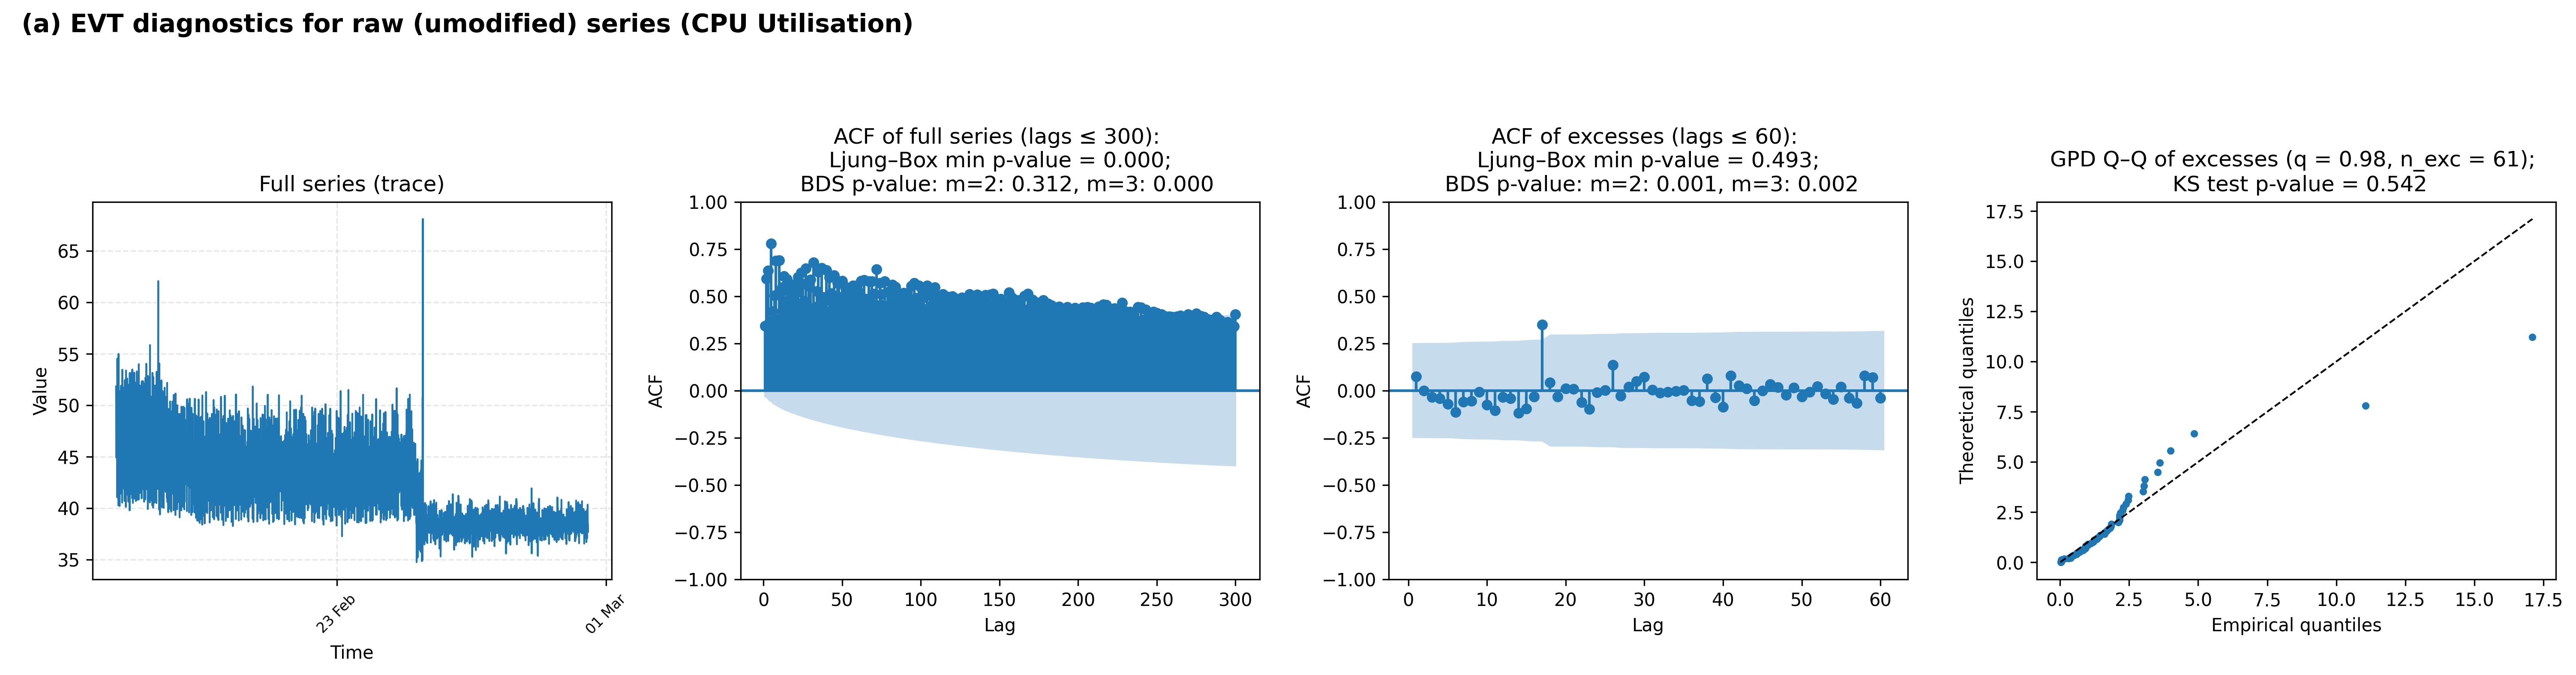
\includegraphics[width=\linewidth]{../output/cpu/evt_raw_diagnostics_cpu.png}\par\vspace{0.35em}
  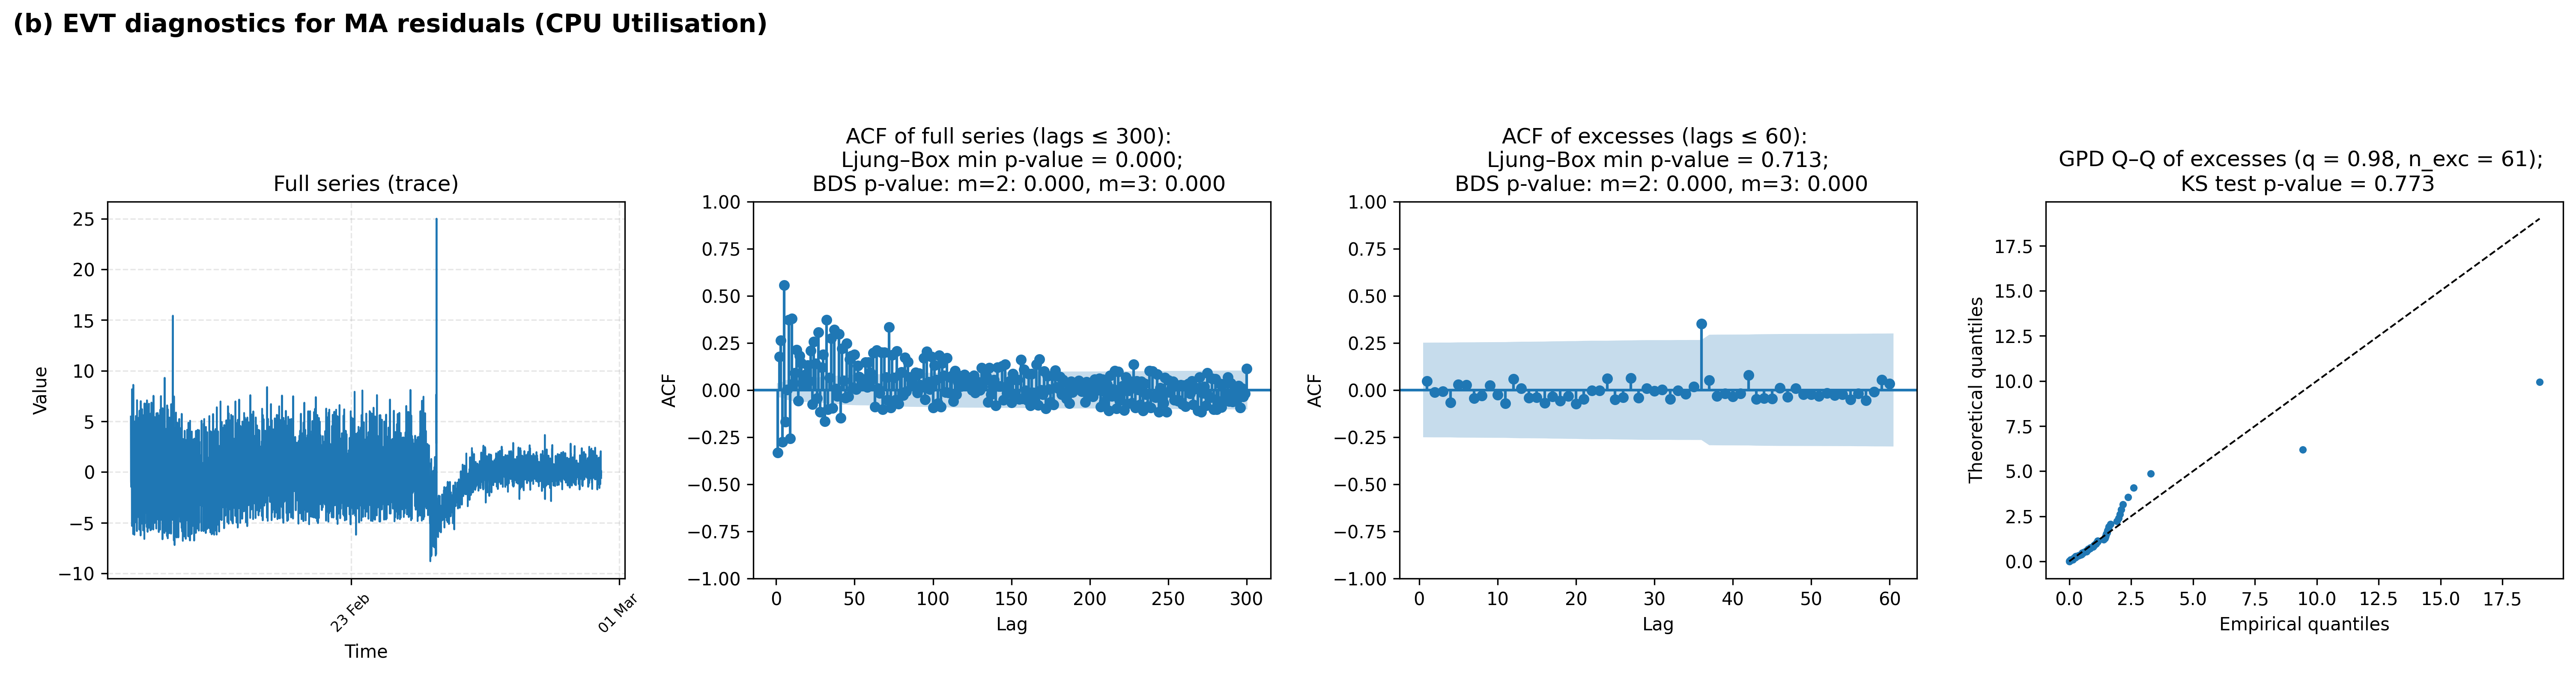
\includegraphics[width=\linewidth]{../output/cpu/evt_ma_diagnostics_cpu.png}\par\vspace{0.35em}
  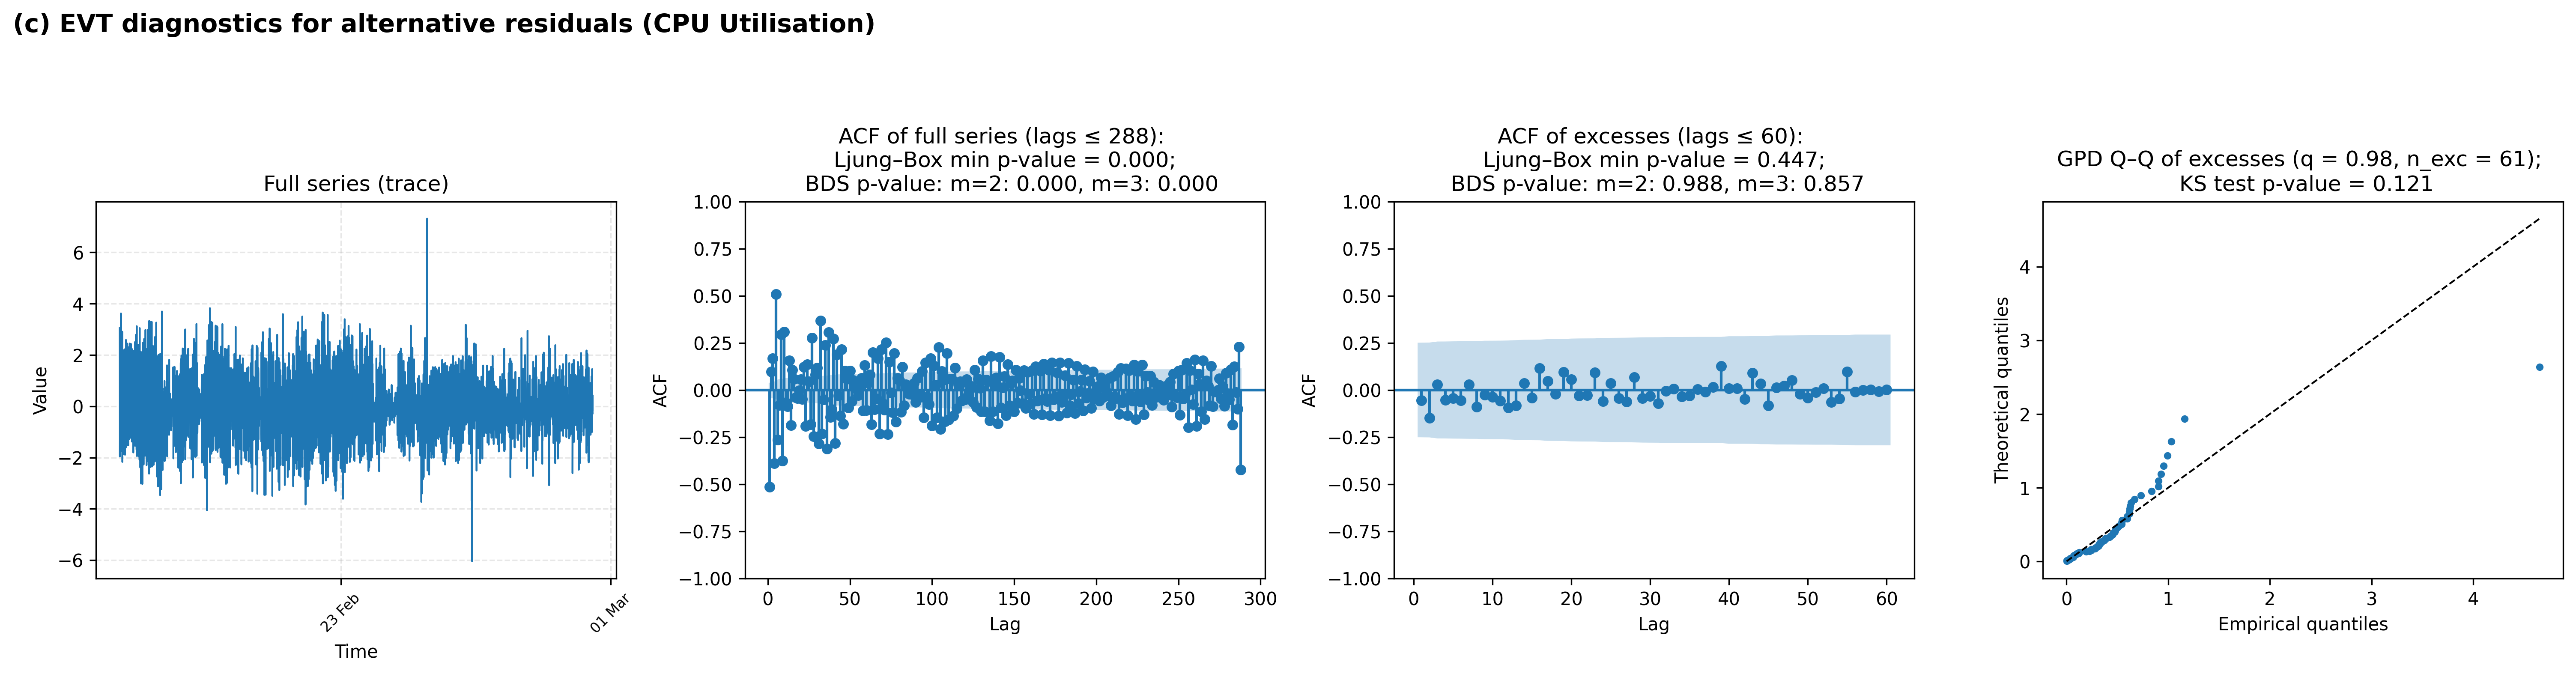
\includegraphics[width=\linewidth]{../output/cpu/evt_prep_diagnostics_cpu.png}
  \caption{EVT diagnostic plots for the CPU Utilisation dataset.}
  \label{fig:prep_cpu}
\end{figure}

\noindent\textbf{CPU Utilisation.} Figure~\ref{fig:prep_cpu} shows that the full raw CPU series is strongly dependent, with the ACF well outside confidence bounds 
and both the Ljung--Box ($p<0.001$). For the BDS test, dependence is detected at $m=3$ ($p=0.001$), though not at $m=2$ ($p=0.312$). 
Raw exceedances are scarce ($n_{\text{exc}}=61$), and while the KS test ($p=0.542$) indicates a broadly acceptable GPD fit, 
the exceedance diagnostics reveal residual structure: the Ljung--Box test ($p=0.493$) does not reject serial independence, 
but the BDS test ($p=0.001$ for $m=2$, $p=0.002$ for $m=3$) points to remaining nonlinear dependence.  
Applying the MA pipeline reduces short-lag autocorrelation in the exceedances and improves the tail fit (KS $p=0.773$), 
though both the full-series and exceedance BDS tests still reject independence. By contrast, the alternative residuals 
achieve near-independence in the extremes (BDS $p=0.988$ at $m=2$, $p=0.857$ at $m=3$), but stronger variance 
stabilisation compresses the largest values, leading to a poorer GPD fit (KS $p=0.121$).  

Overall, the CPU series illustrates a clear trade-off between tail fit and independence: the MA residuals yield the 
strongest GPD conformity but retain residual dependence, whereas the alternative residuals better approximate 
independence at the cost of a weaker tail model. This contrast highlights the differing priorities of basic POT detection, 
which benefits from well-calibrated GPD tails, versus EQD-enhanced approaches, which are expected to gain more from 
the reduced dependence offered by the alternative residuals.

\begin{figure}[ht]
  \centering
  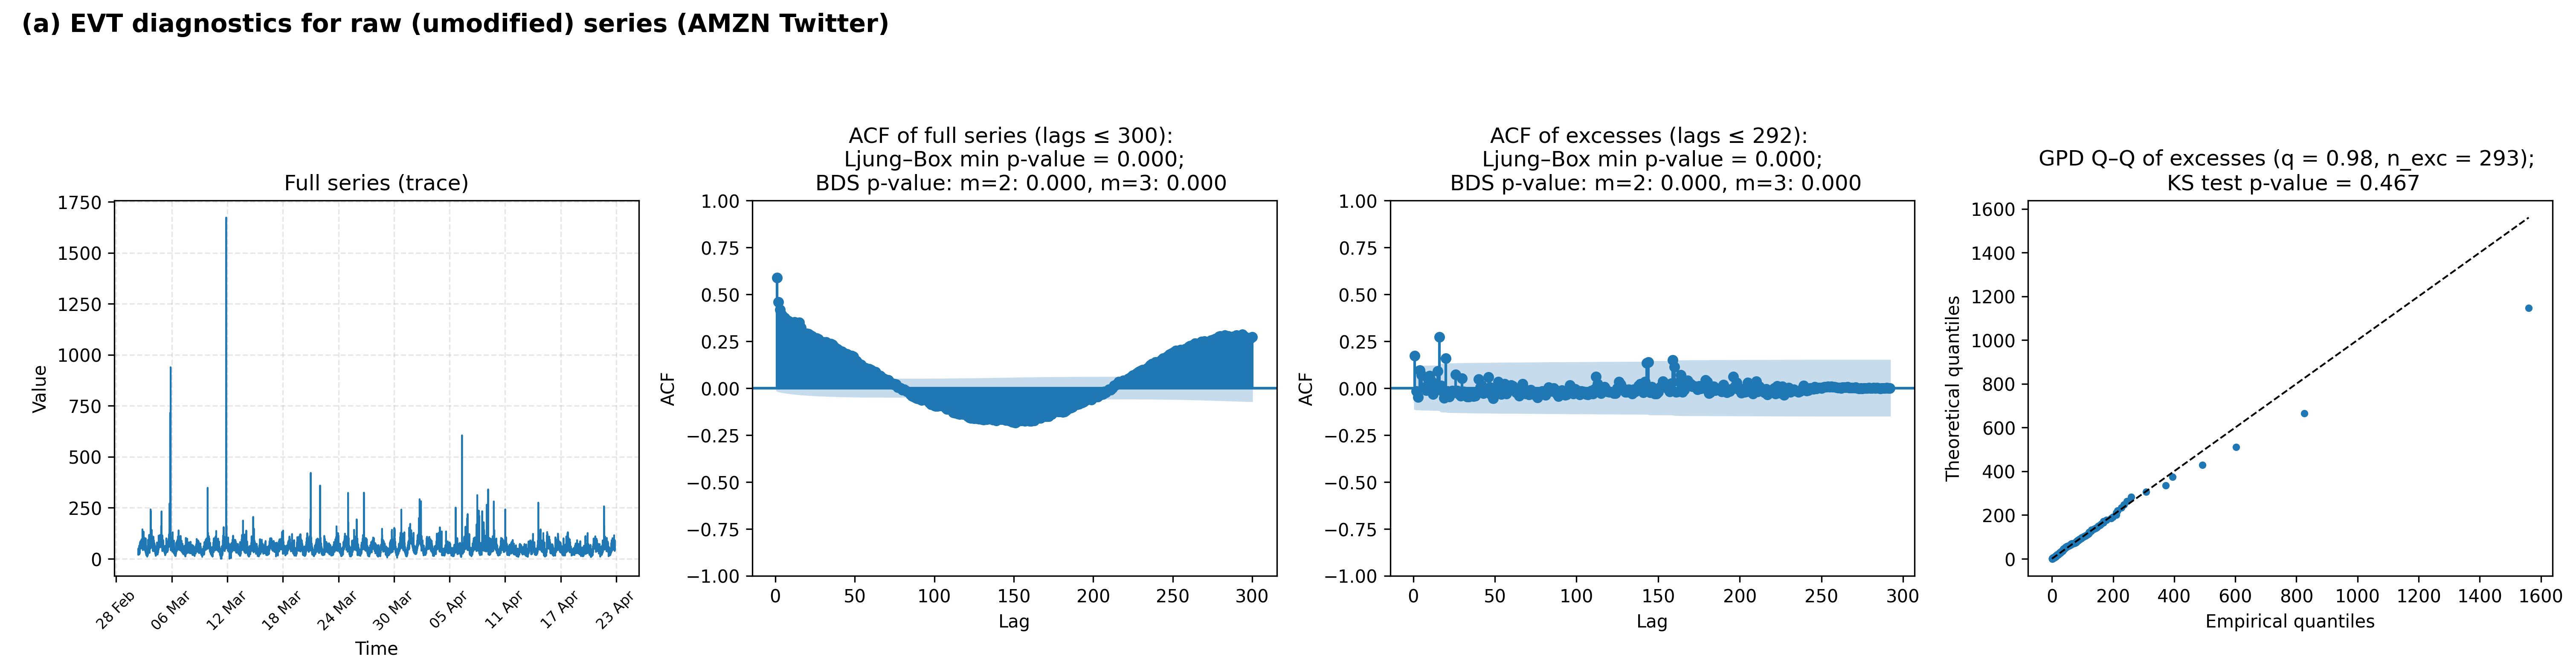
\includegraphics[width=\linewidth]{../output/realTweets/evt_raw_diagnostics_realTweets.png}\par\vspace{0.35em}
  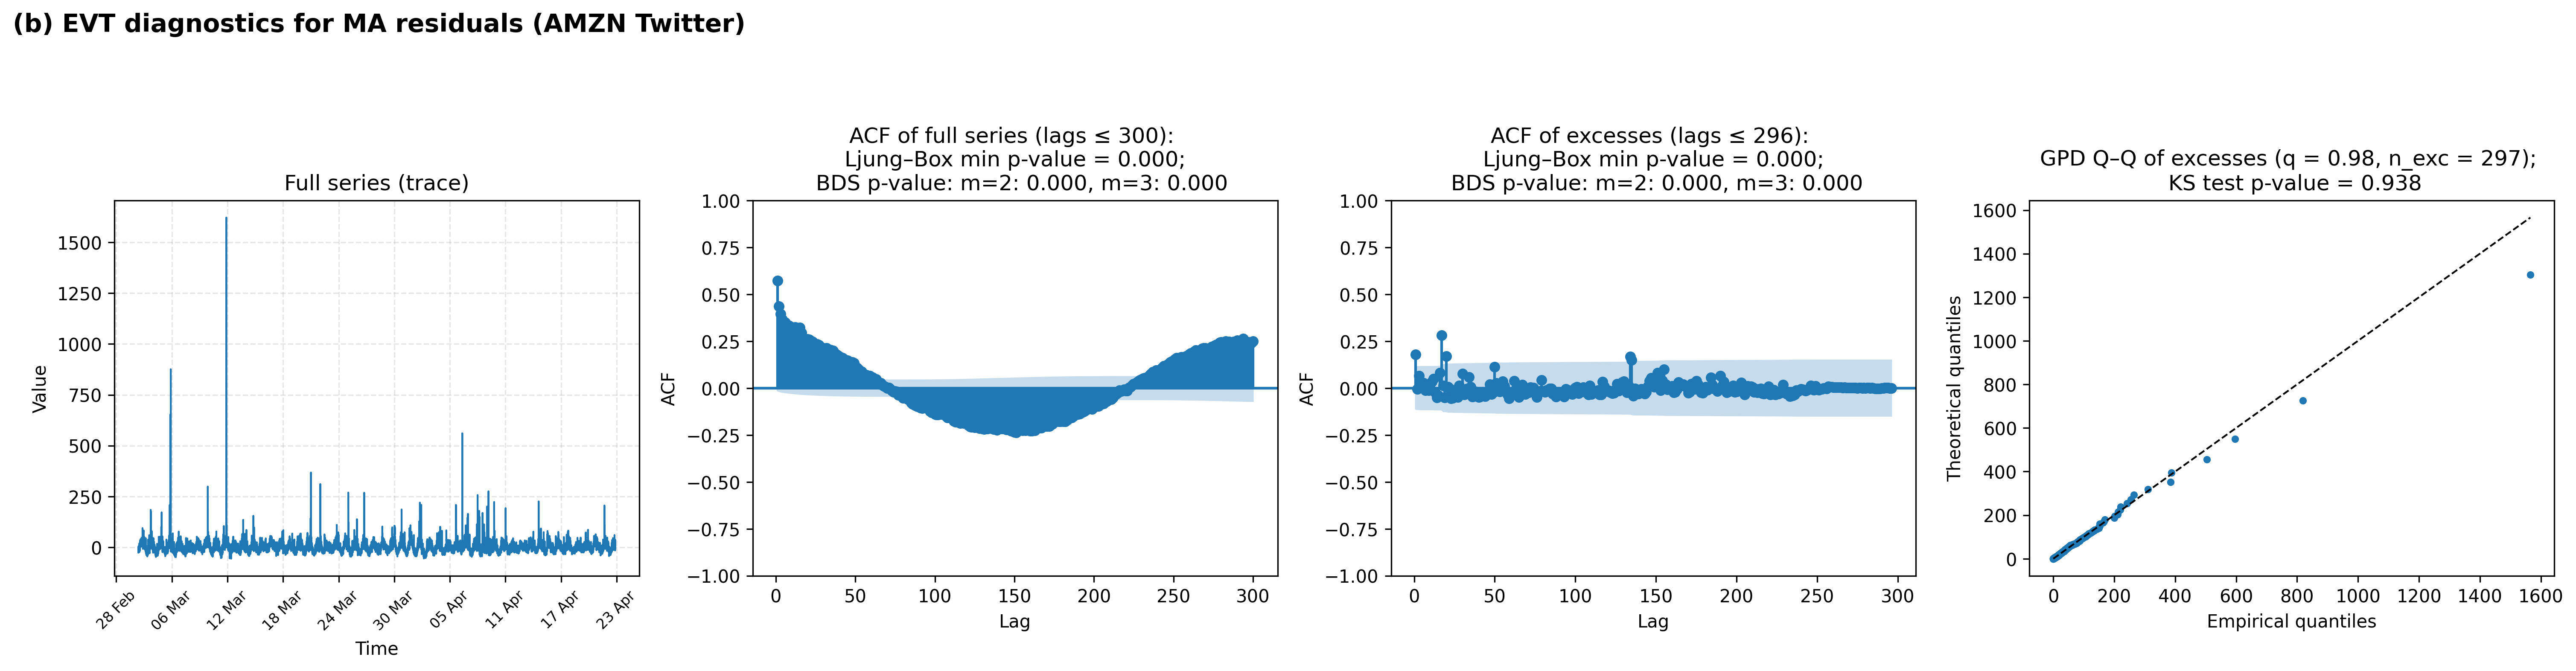
\includegraphics[width=\linewidth]{../output/realTweets/evt_ma_diagnostics_realTweets.png}\par\vspace{0.35em}
  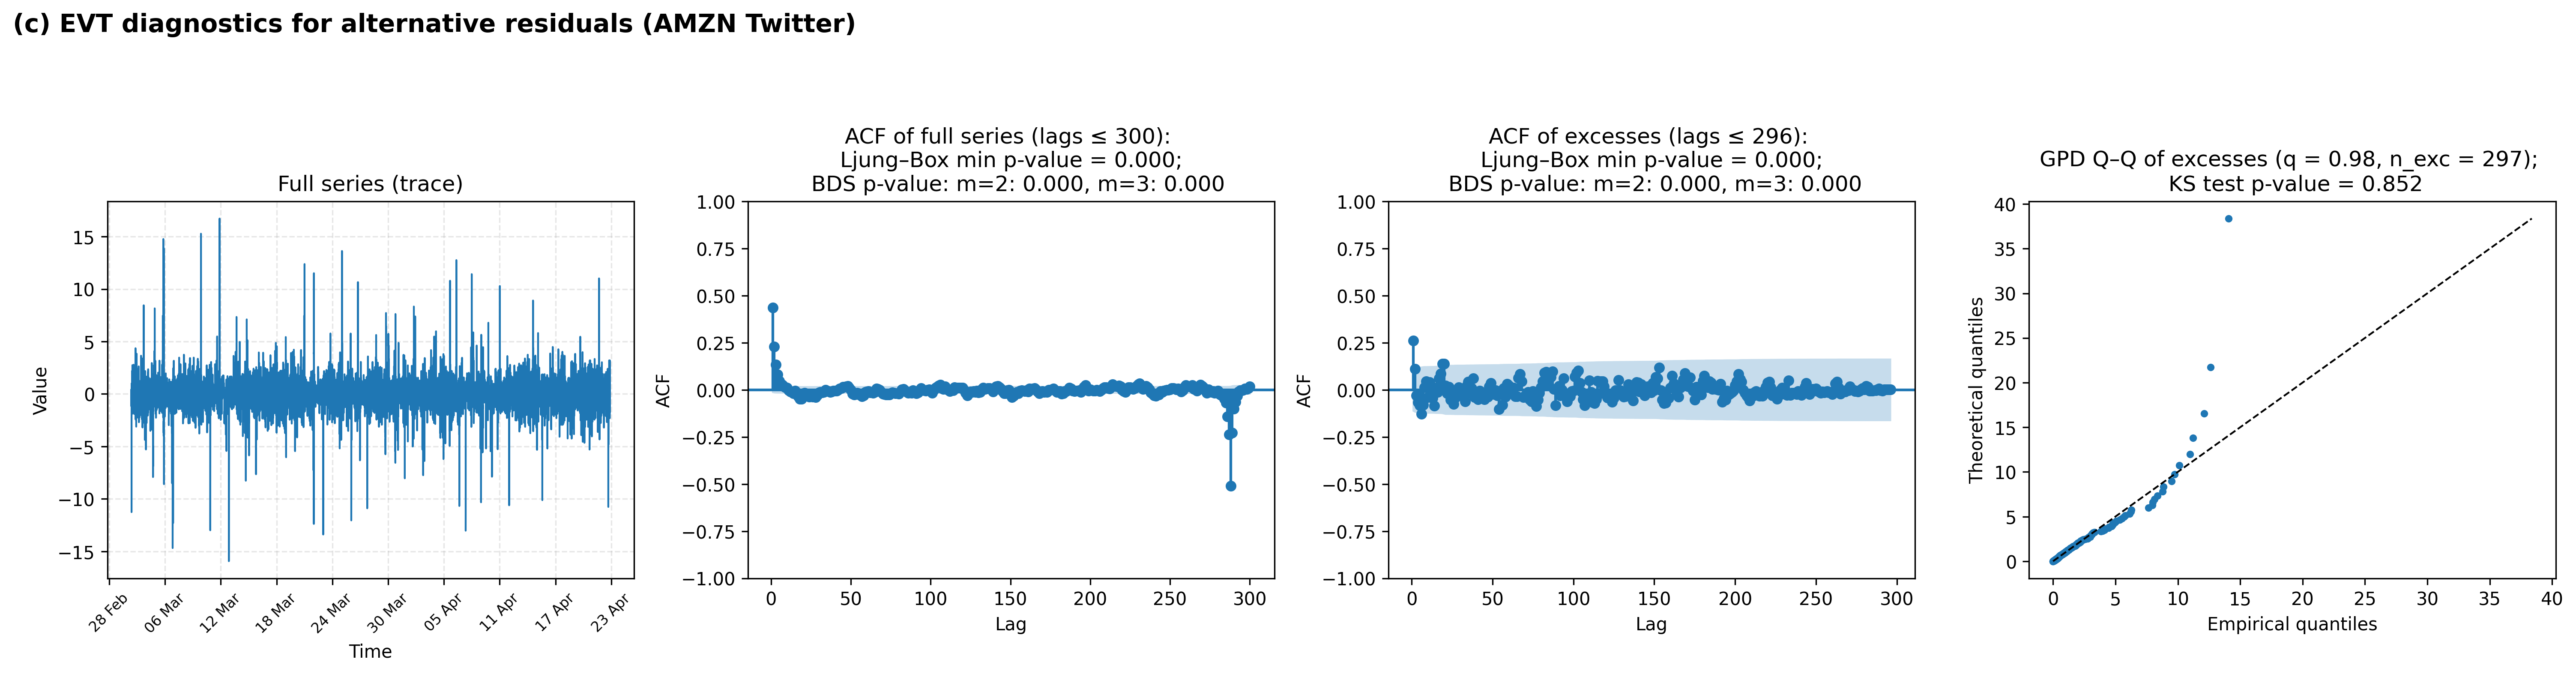
\includegraphics[width=\linewidth]{../output/realTweets/evt_prep_diagnostics_realTweets.png}
  \caption{EVT diagnostic plots for the AMZN Twitter dataset.}
  \label{fig:prep_twitter}
\end{figure}

\noindent\textbf{AMZN Twitter.} Figure~\ref{fig:prep_twitter} shows that the raw Twitter series exhibits very strong dependence, with the ACF remaining 
significant over hundreds of lags and both the Ljung--Box and BDS tests decisively rejecting independence ($p<0.001$). 
Applying the MA pipeline does little to improve these diagnostics, as both tests again reject, but it does yield a notably 
stronger GPD tail fit (KS $p=0.938$). The alternative pipeline suppresses variance fluctuations more aggressively, 
yet the dependence diagnostics remain unchanged: both tests continue to reject for the full series and for exceedances. 
The KS fit is only marginally weaker ($p=0.852$), reflecting lighter tails induced by stronger variance stabilisation, 
but still indicates a valid GPD model. 

Overall, these results confirm that even with enhanced preprocessing, the Twitter data retain substantial dependence, 
including in the exceedances. This limits the expected gains from EQD, since the preprocessing alone does not yield 
near-i.i.d.\ series. In practice, we may still expect the alternative residuals to lower false positives compared 
to MA preprocessing by stabilising variance, but the persistence of serial dependence means that POT-based detection 
is unlikely to achieve its full theoretical robustness here, and EQD is unlikely to offer substantial additional benefit.

\begin{figure}[ht]
  \centering
  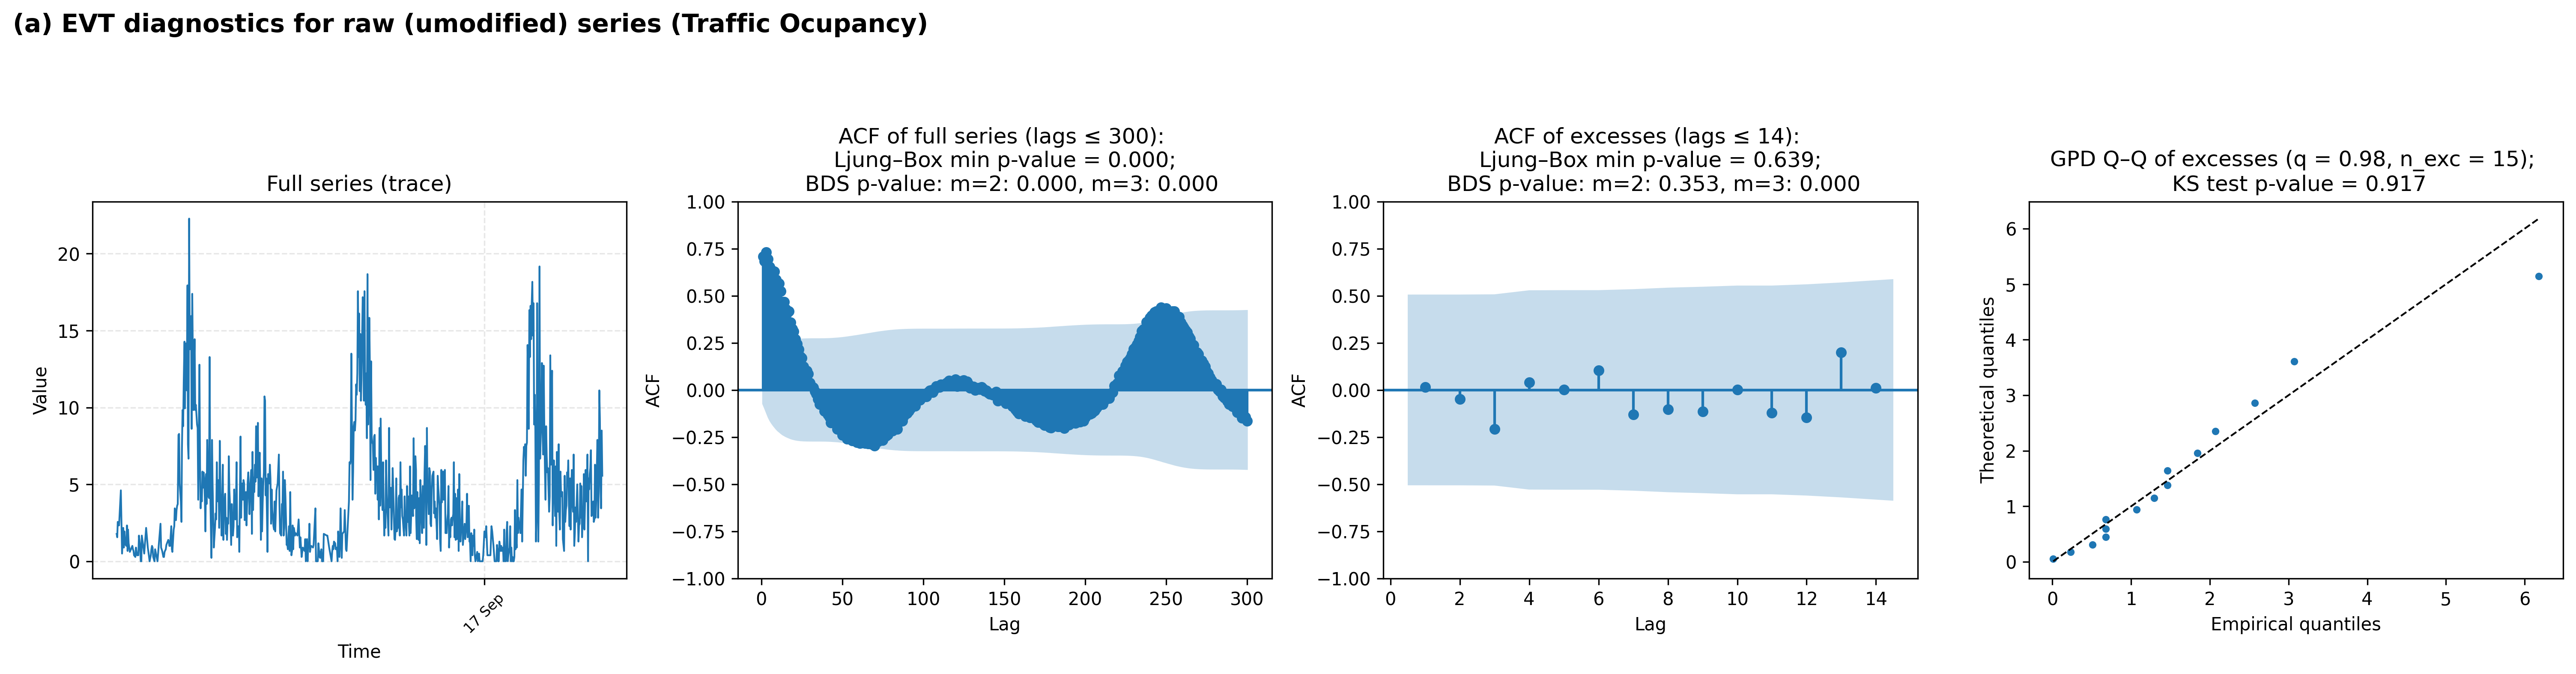
\includegraphics[width=\linewidth]{../output/occupancy/evt_raw_diagnostics_occupancy.png}\par\vspace{0.35em}
  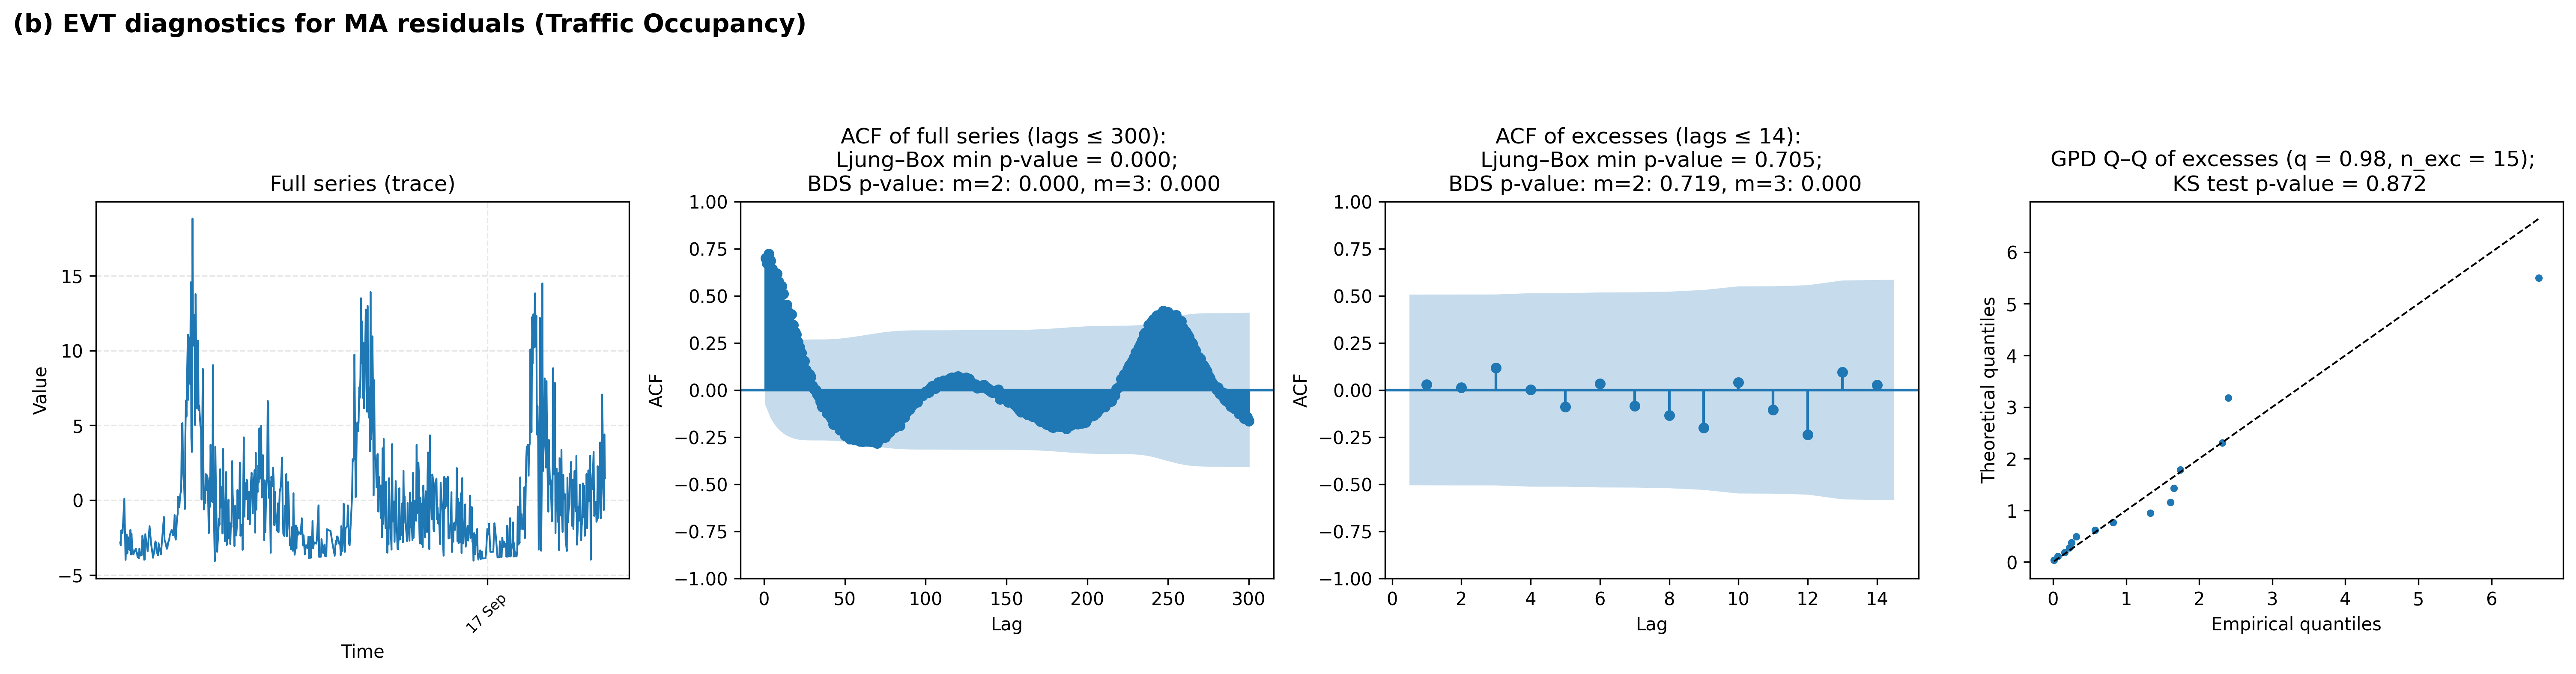
\includegraphics[width=\linewidth]{../output/occupancy/evt_ma_diagnostics_occupancy.png}\par\vspace{0.35em}
  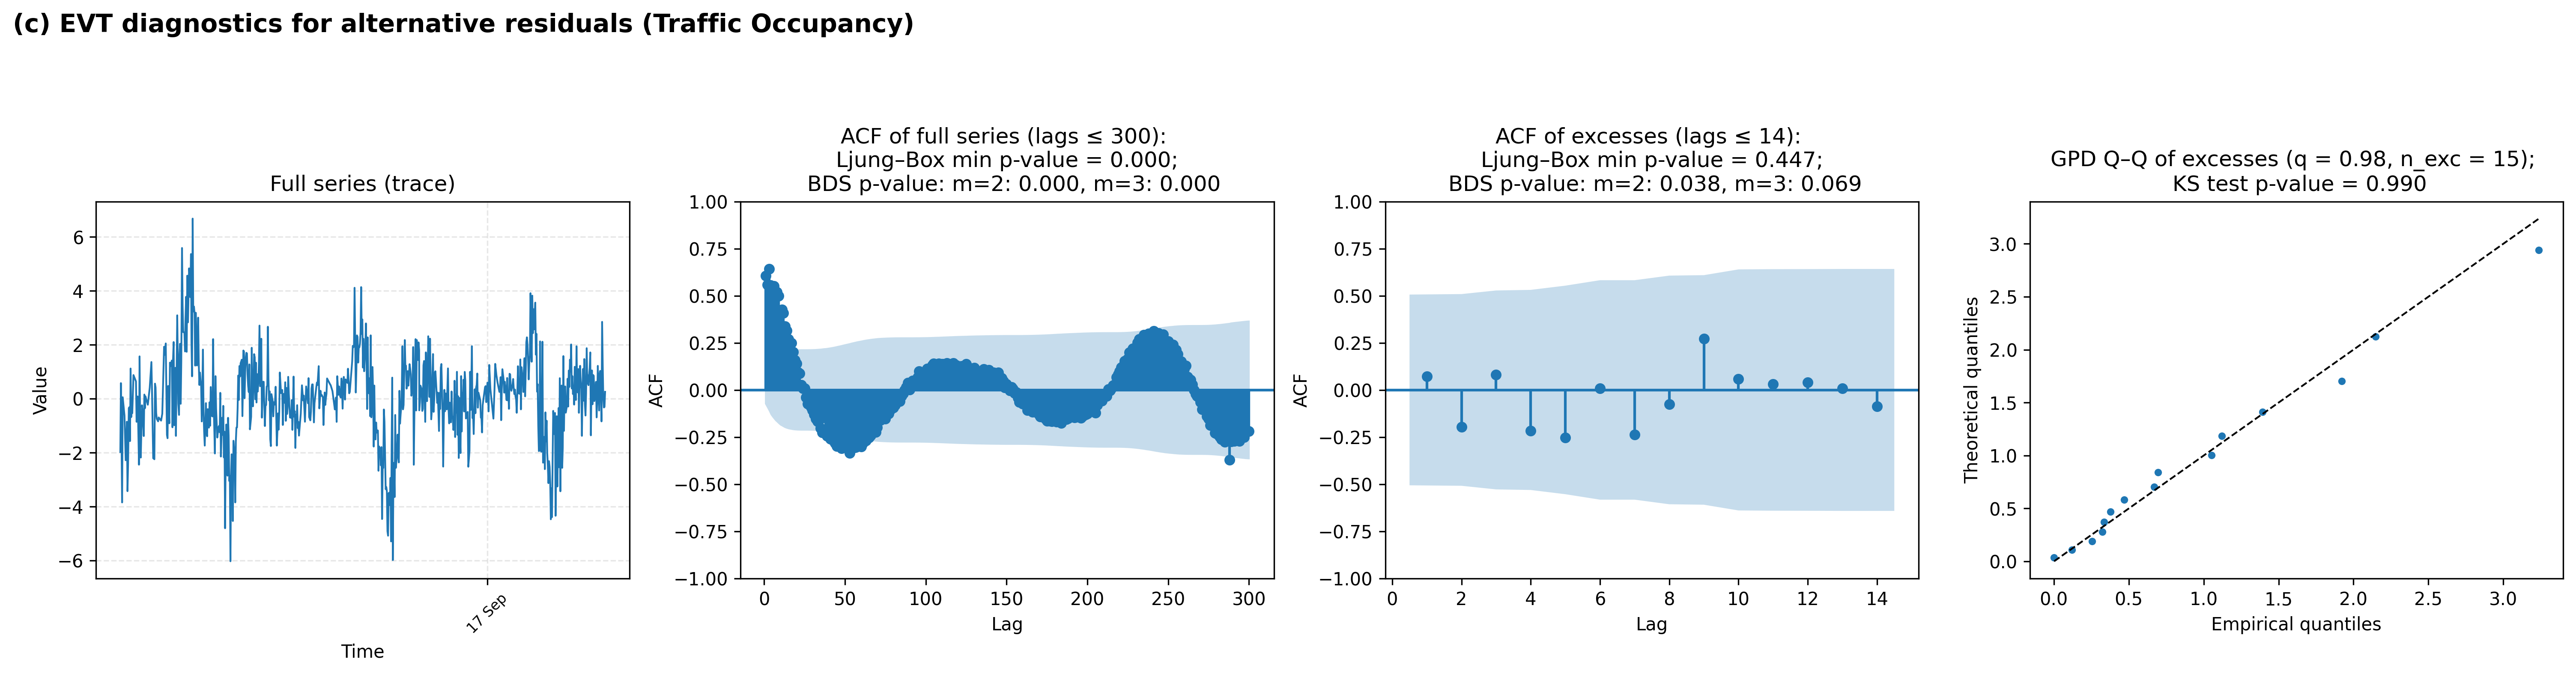
\includegraphics[width=\linewidth]{../output/occupancy/evt_prep_diagnostics_occupancy.png}
  \caption{EVT diagnostic plots for the Traffic Occupancy dataset.}
  \label{fig:prep_occupancy}
\end{figure}

\noindent\textbf{Traffic Occupancy.} Figure~\ref{fig:prep_occupancy} highlights a strong periodic structure in the raw series, with oscillating ACFs and both tests 
rejecting independence ($p<0.001$). Exceedance dependence shows mixed results: the Ljung--Box test is non-significant ($p=0.639$) and the BDS test does not reject 
at $m=2$ ($p=0.353$), but independence is rejected at $m=3$ ($p=0.000$), indicating residual higher-order nonlinear dependence. 
Nonetheless, the GPD tail fit is already strong (KS $p=0.917$). MA preprocessing shortens autocorrelations, with the Ljung--Box 
improving slightly ($p=0.705$), though weak nonlinear dependence remains (BDS $p=0.719$ for $m=2$, $p=0.000$ for $m=3$). The tail
fit is preserved (KS $p=0.872$). The alternative residuals deliver the clearest gains in the exceedances: while the Ljung--Box 
remains non-significant ($p=0.447$), the BDS test now yields borderline outcomes ($p=0.038$ at $m=2$ and $p=0.069$ at $m=3$), 
indicating weak evidence of dependence at the 5\% level. At the same time, the GPD fit is excellent (KS $p=0.990$).

Overall, these diagnostics suggest that the enhanced pipeline offers the most favourable trade-off between approximate 
independence and tail stability for this dataset. While some residual dependence remains, the alternative residuals 
provide clear improvements over both the raw and MA-processed series. In such settings, the EQD-enhanced approach may add 
robustness by further safeguarding threshold specification under the residual periodic structure.

\subsection{Comparative Results of DSPOT Variants Across Datasets}\label{subsec:main_results}

We now turn to the central performance comparison of the four detection variants applied to each dataset: 
\begin{enumerate}
  \renewcommand{\labelenumi}{(\alph{enumi})}
  \item DSPOT on MA residuals with default threshold;
  \item DSPOT on MA residuals with EQD-enhanced threshold;
  \item Modified DSPOT on alternative residuals with default threshold;
  \item Modified DSPOT on alternative residuals with EQD-enhanced threshold.
\end{enumerate}
The goal is to assess whether more complex alternative preprocessing and threshold selection yield tangible benefits 
at the event level evaluation as described in Section~\ref{subsec:event_ev}. As discussed in Section~\ref{subsec:evt_diagnostic}, 
the datasets vary markedly in how well their residuals approximate the i.i.d.\ conditions assumed by POT; this provides a 
principled basis for evaluating the robustness of each variant. Results are summarised in 
Tables~\ref{tab:cpu_event_metrics}--\ref{tab:traffic_event_metrics} 
and Figures~\ref{fig:evt_ad_cpu}--\ref{fig:evt_ad_traffic}.

\begin{figure}[ht]
  \centering
  \begin{minipage}{0.48\linewidth}
    \centering
    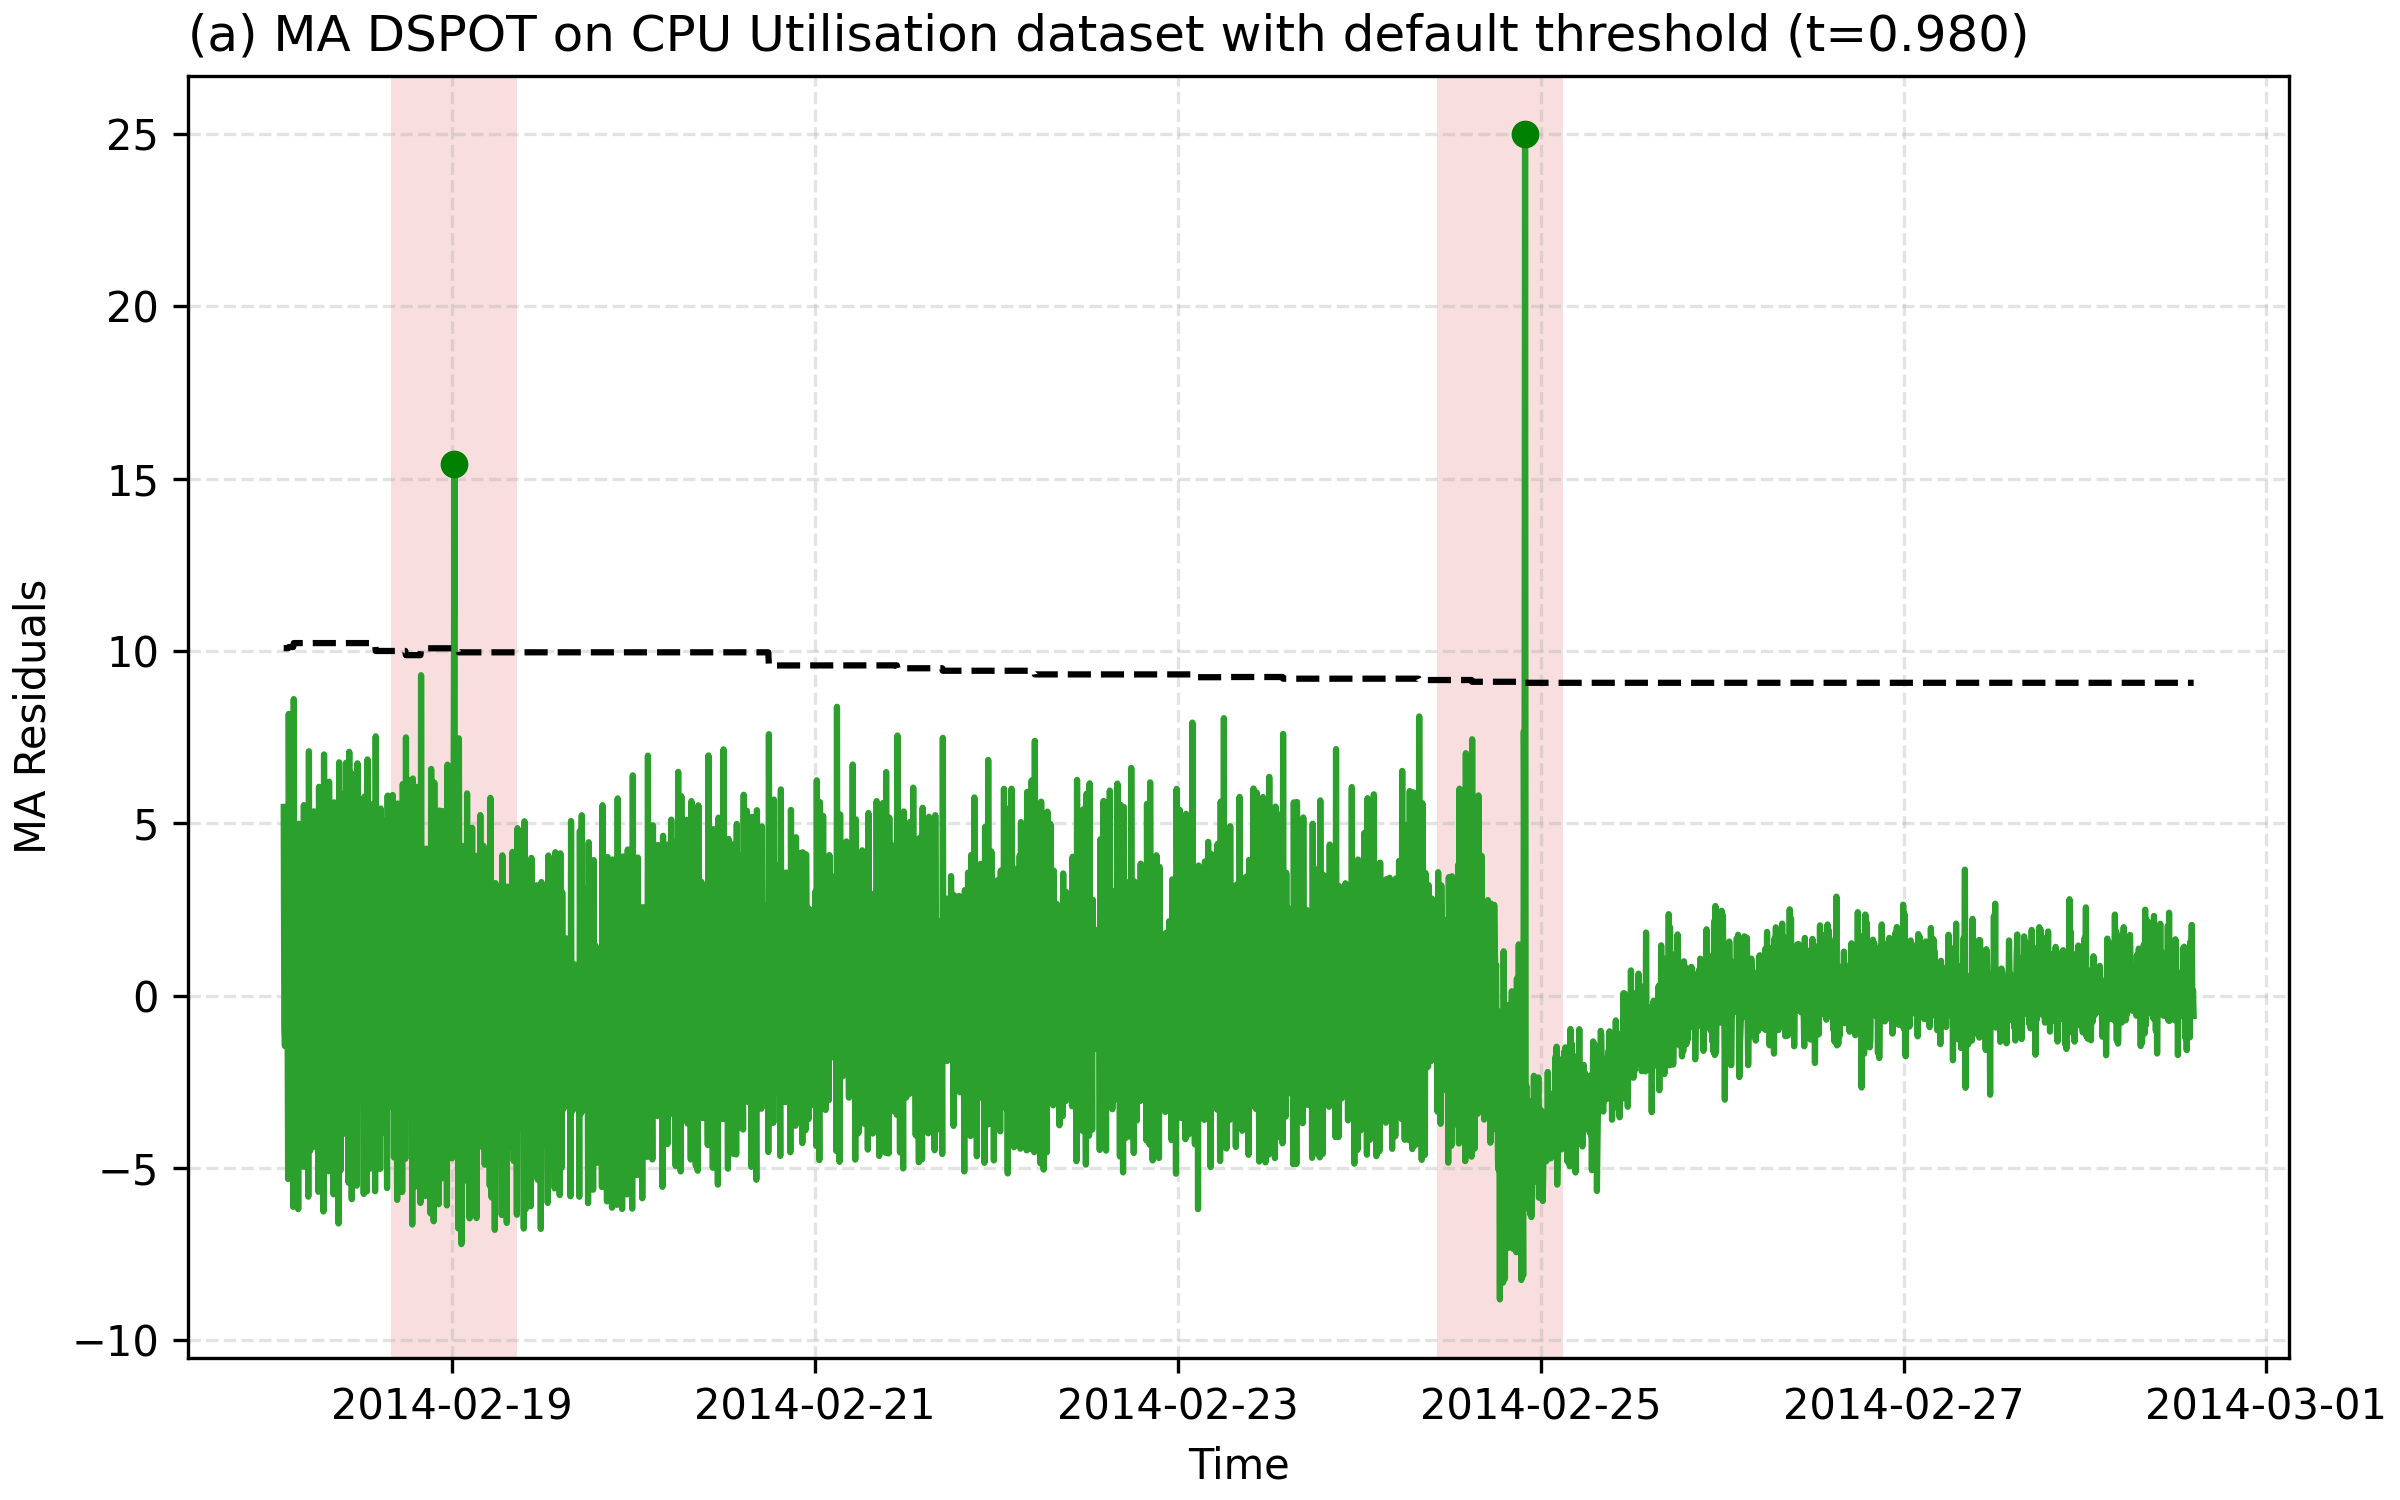
\includegraphics[width=\linewidth]{../output/cpu/original_dspot_cpu.png}
    \vspace{0.35em}
    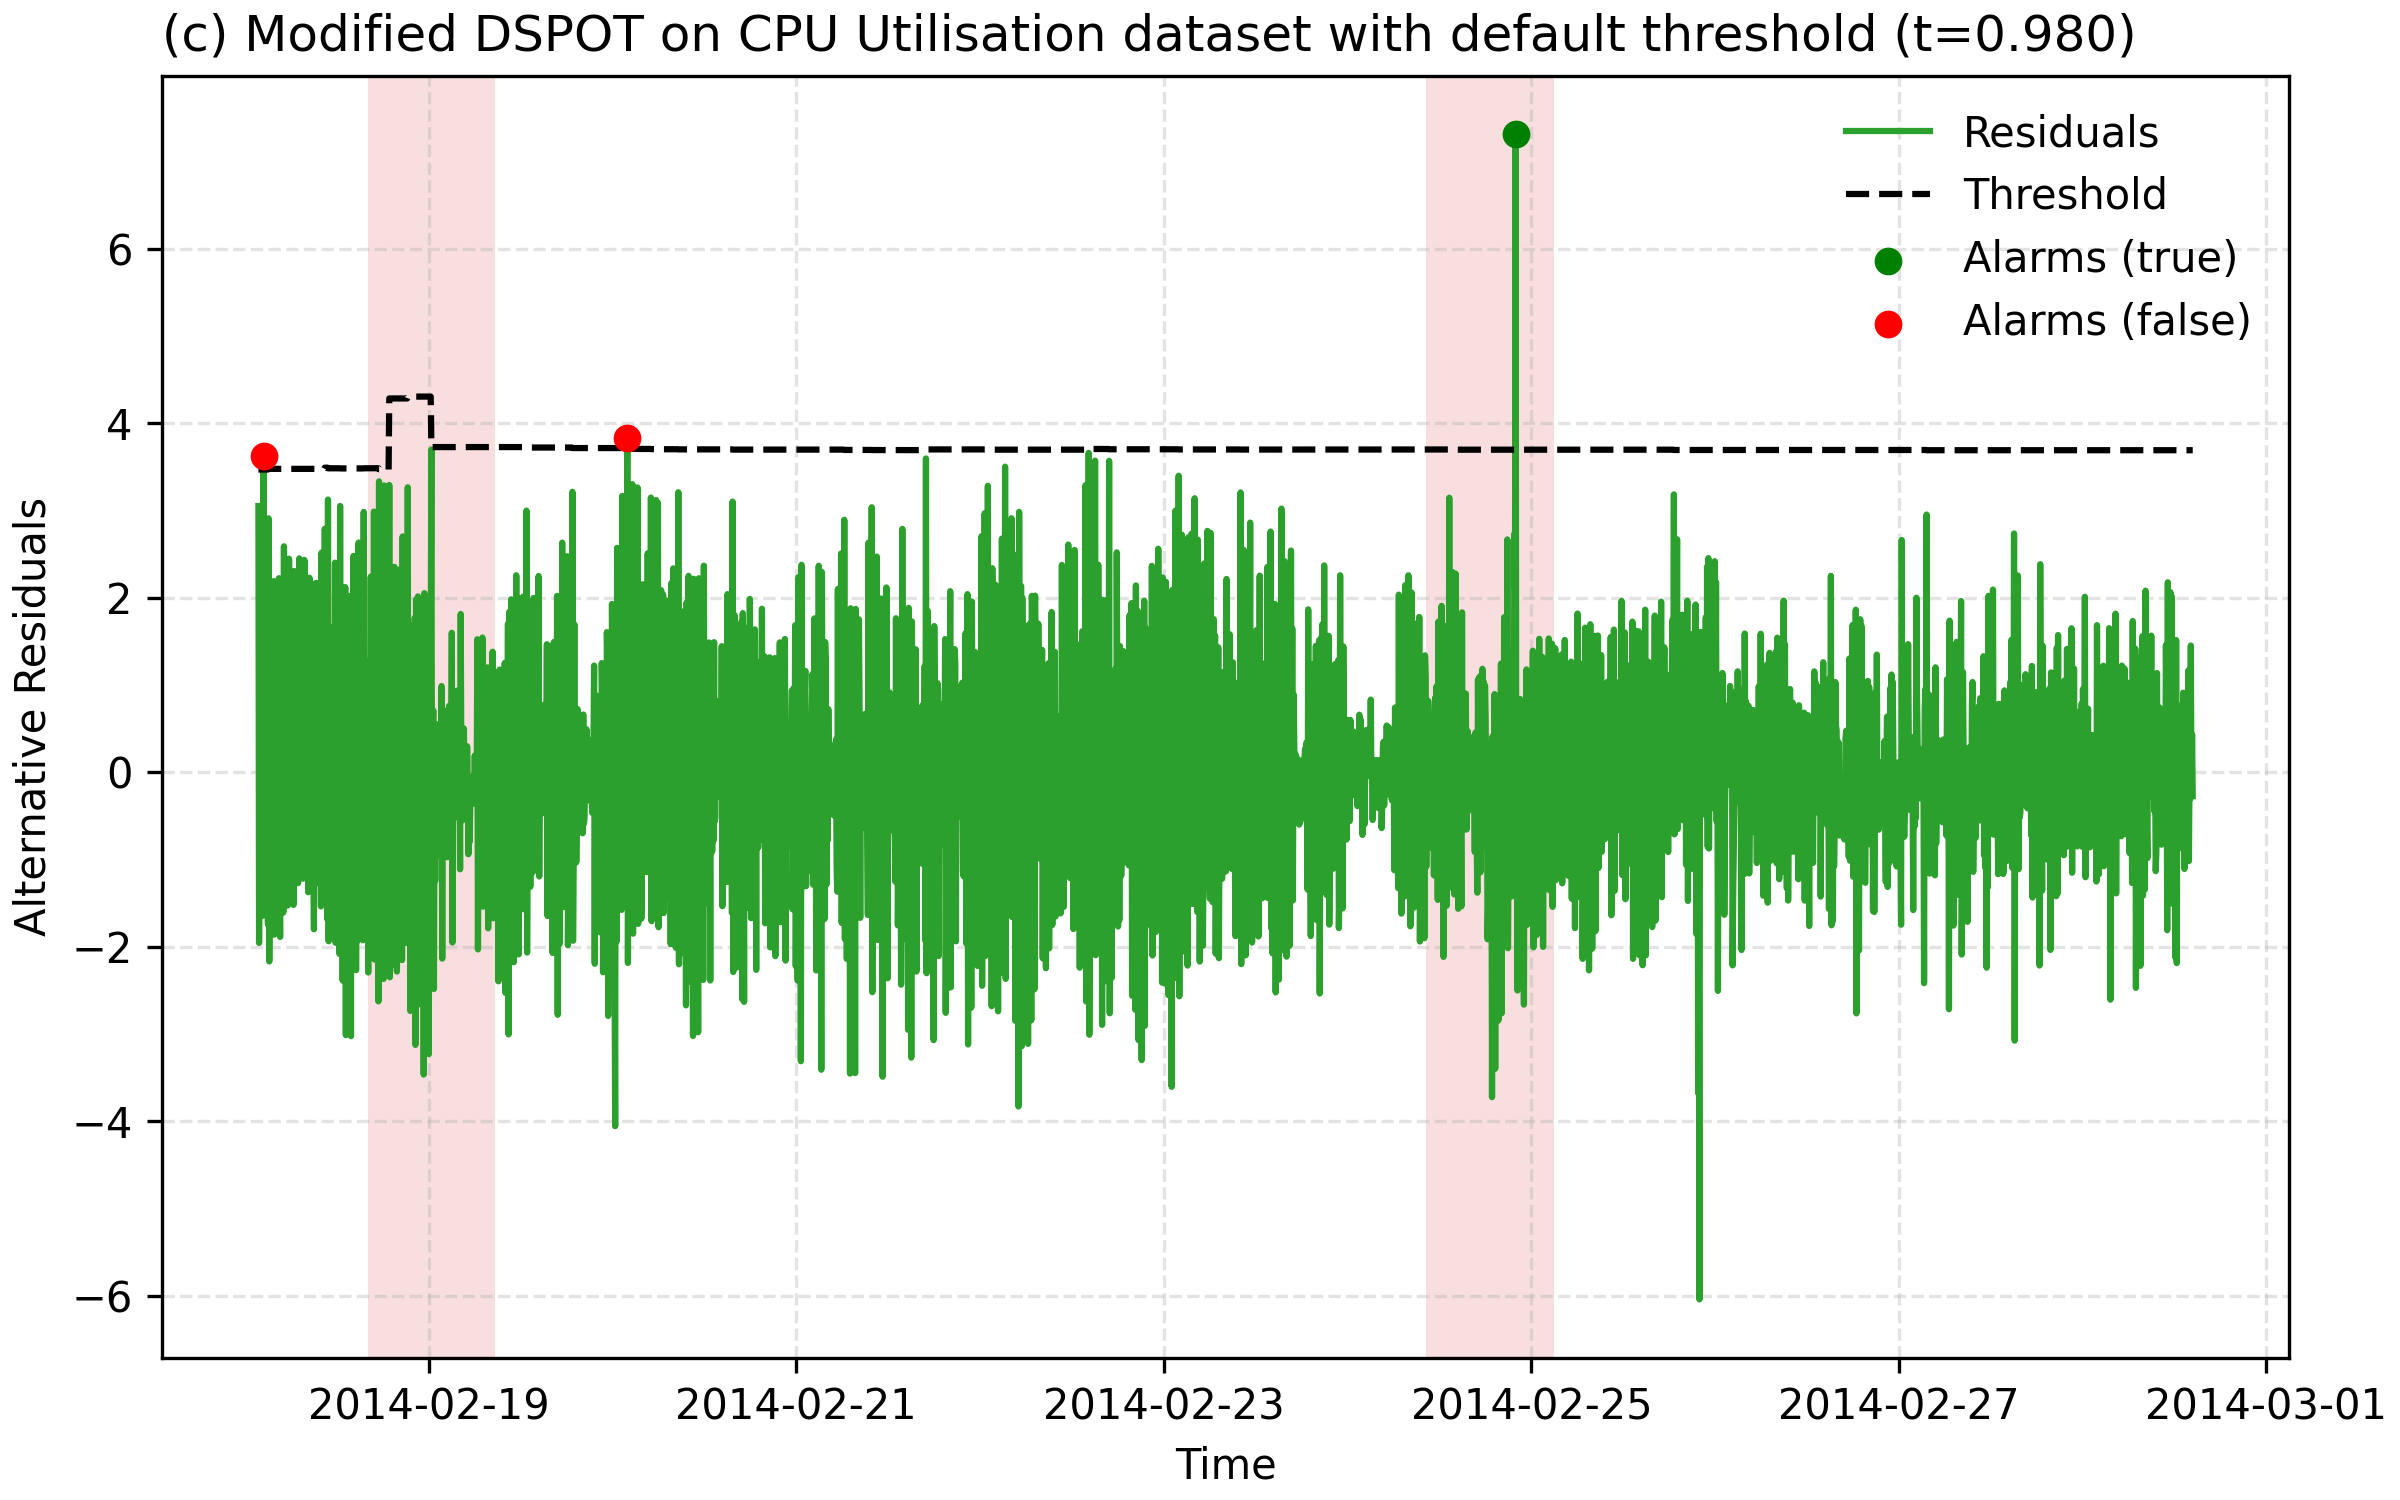
\includegraphics[width=\linewidth]{../output/cpu/preprocessed_spot_cpu.png}
  \end{minipage}\hfill
  \begin{minipage}{0.48\linewidth}
    \centering
    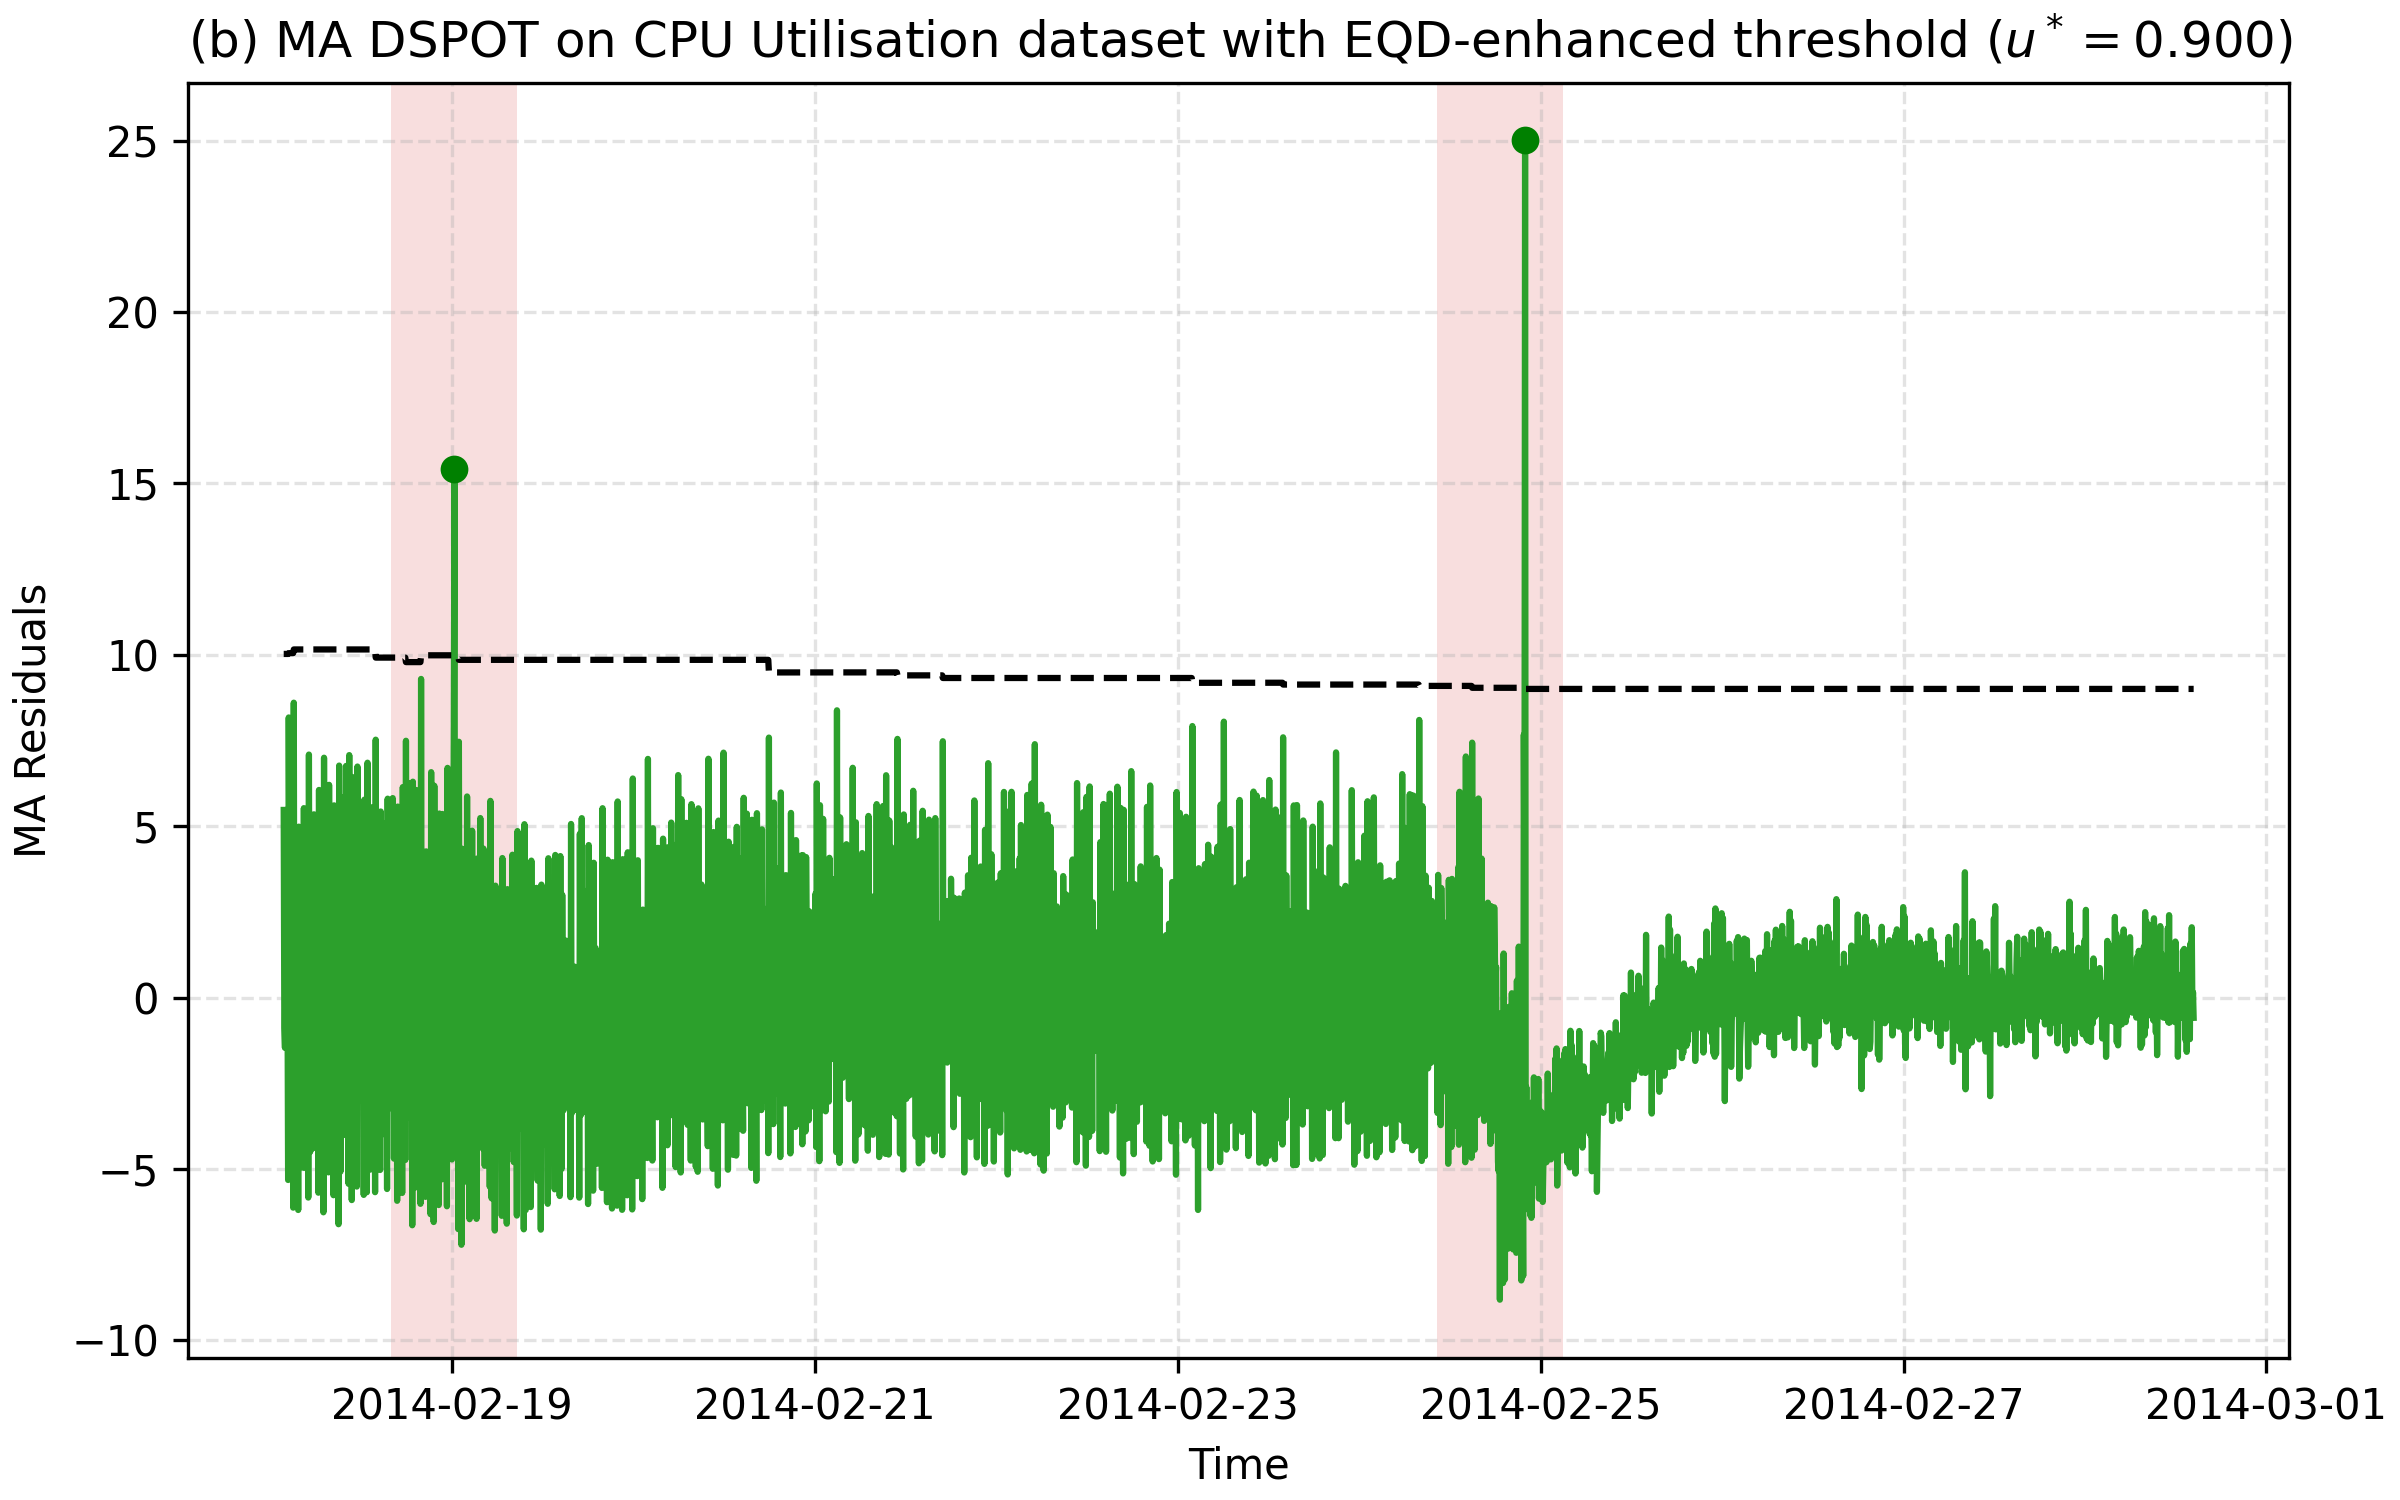
\includegraphics[width=\linewidth]{../output/cpu/optimal_threshold_dspot_cpu.png}
    \vspace{0.35em}
    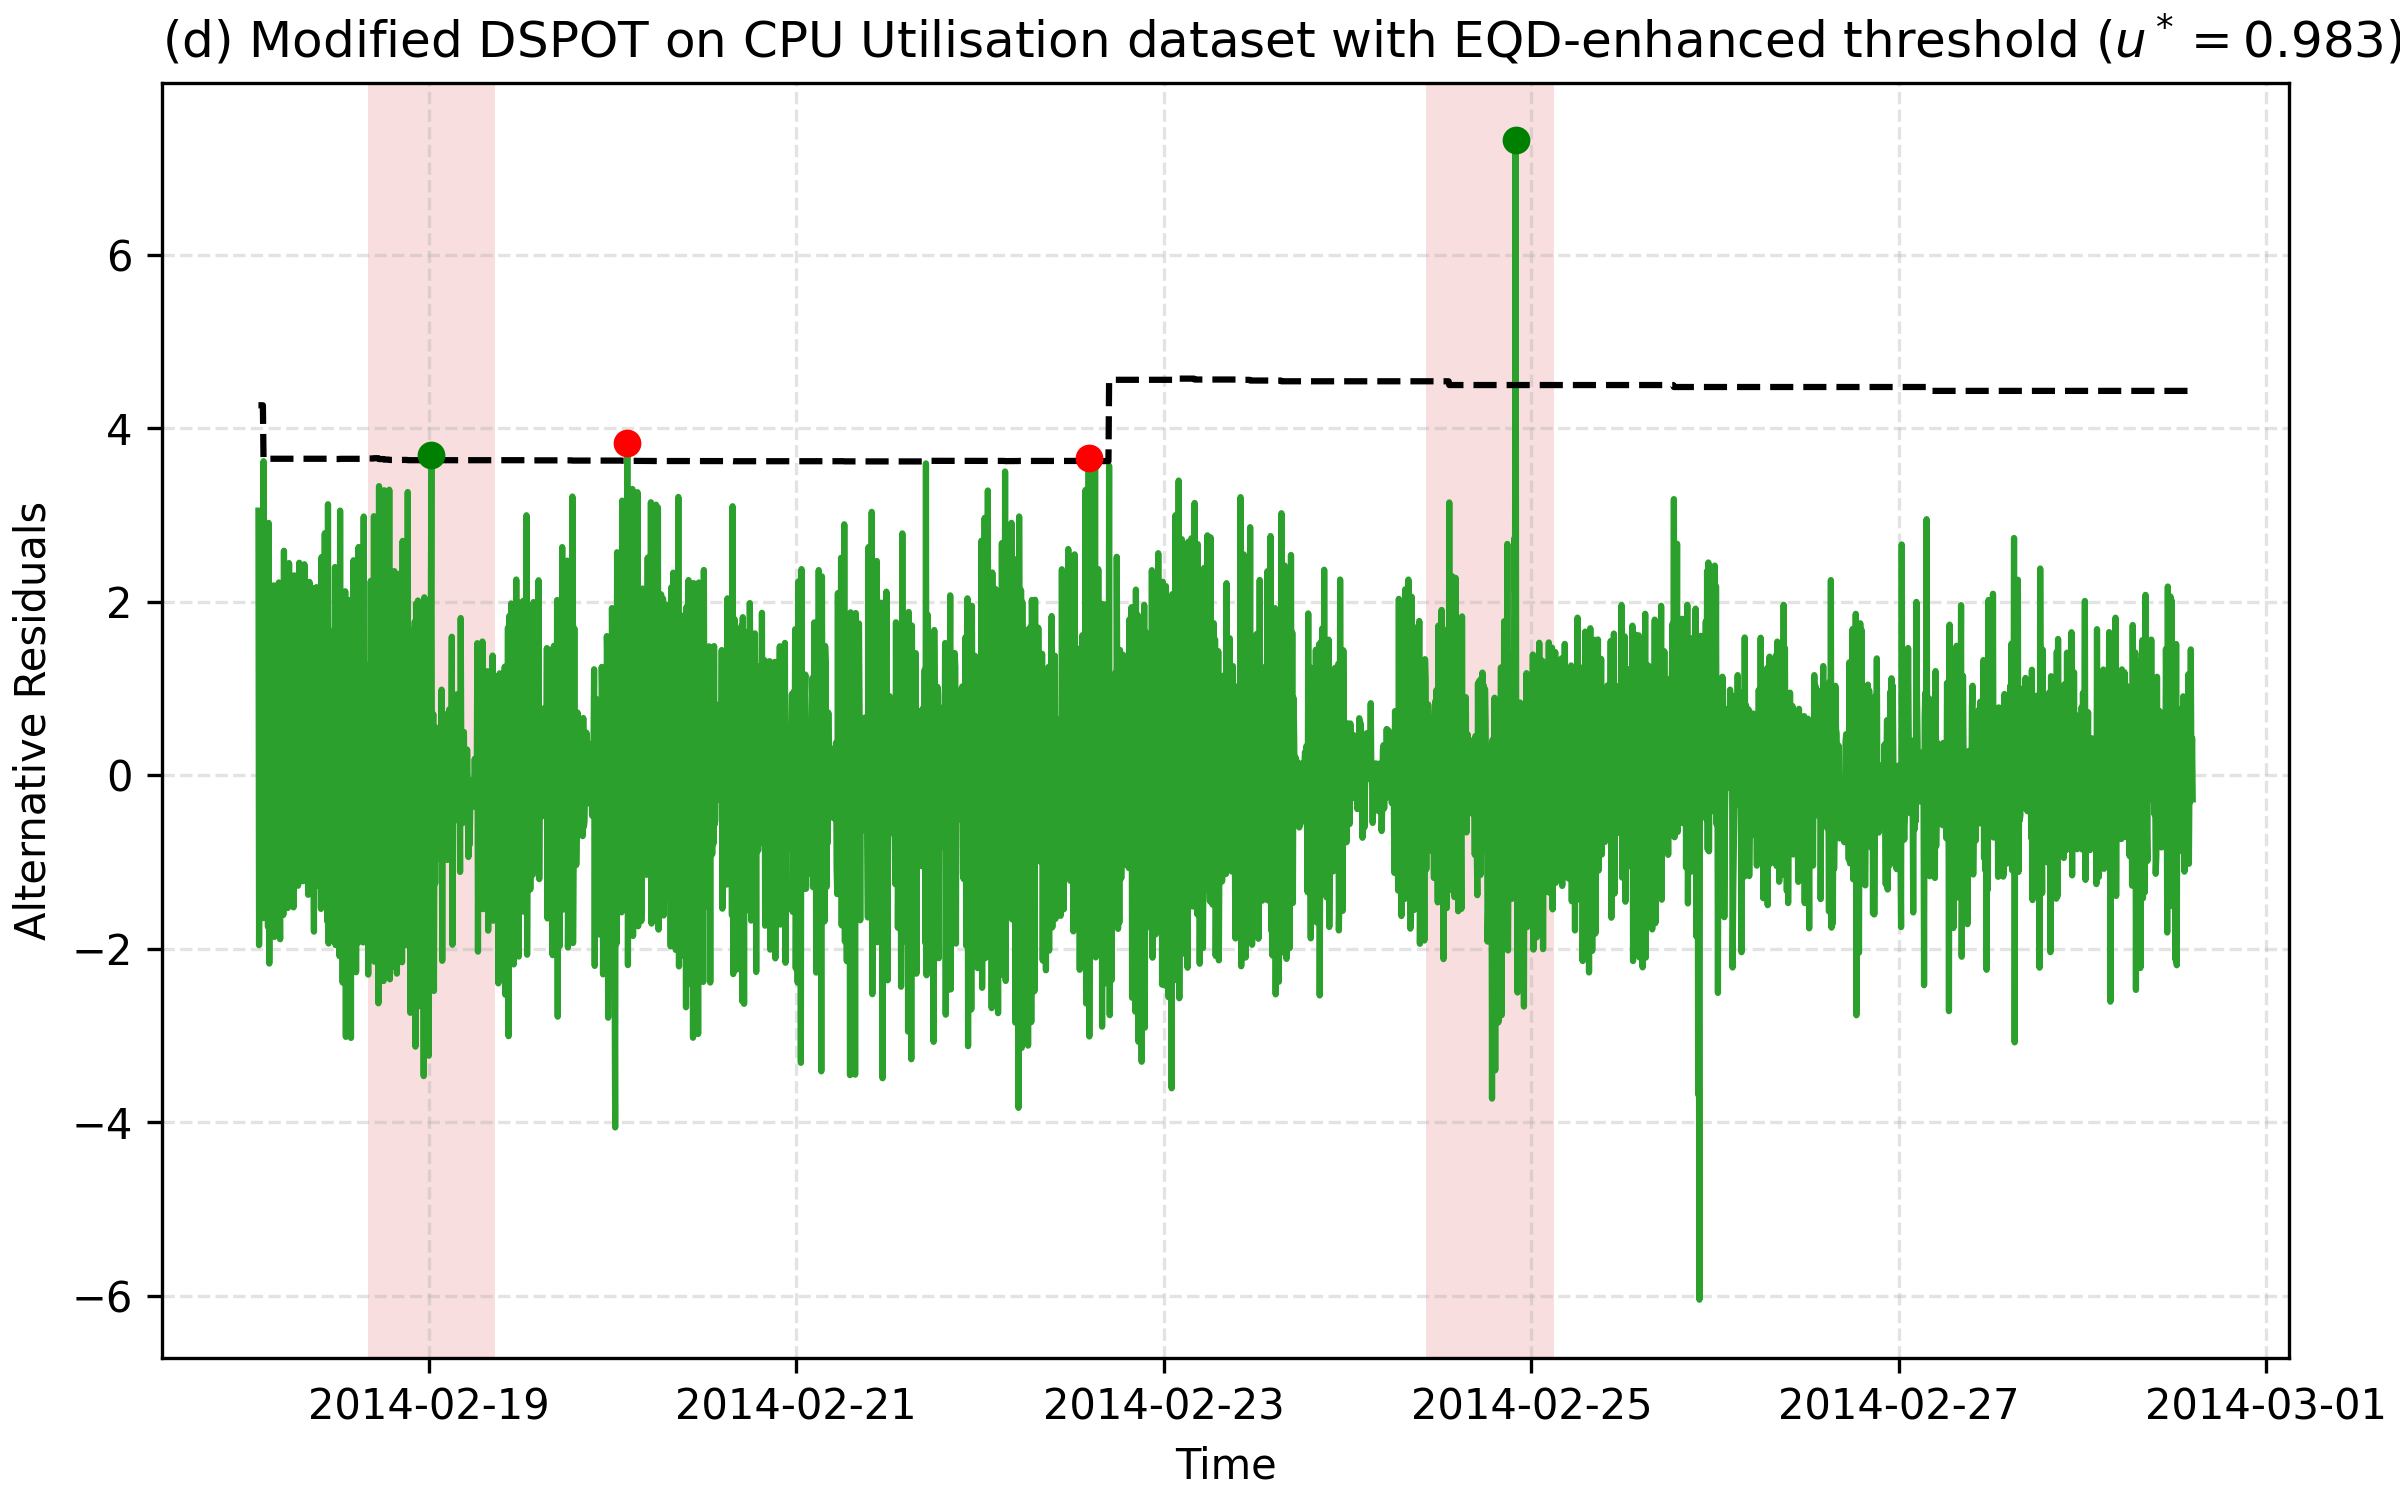
\includegraphics[width=\linewidth]{../output/cpu/optimal_threshold_preprocessed_spot_cpu.png}
  \end{minipage}
  \caption{Anomaly detection results on the CPU Utilisation dataset. 
  Each panel shows residuals, dynamic thresholds (dashed), and alarm events (dots) under the four DSPOT variants: 
  (a) MA residuals with default threshold, (b) MA residuals with EQD-enhanced threshold, 
  (c) alternative residuals with default threshold, and (d) alternative residuals with EQD-enhanced threshold. 
  Shaded bands indicate ground-truth anomaly windows.}
  \label{fig:evt_ad_cpu}
\end{figure}

\noindent\textbf{CPU Utilisation.} The CPU dataset is structurally simple, characterised by a single abrupt level shift 
and otherwise stable variance with only minor stochastic fluctuations. Table~\ref{tab:cpu_event_metrics} shows that both 
DSPOT variants on MA residuals (a and b) achieve perfect classification of the two anomaly windows, with no false alarms and 
a median delay of 600 minutes. This delay should be interpreted in the context of the wide ground-truth anomaly windows, 
which span many hours, so that detection still occurs well within the event duration. In this setting, EQD-enhancement produces
no observable benefit: although it selects a lower threshold ($u^*=0.9$) and earlier diagnostics did not provide strong evidence 
that the exceedances are i.i.d., the anomalies are so pronounced that DSPOT already yields perfect results, regardless of 
threshold refinement. By contrast, the modified DSPOT 
on alternative residuals (c and d) suffers from over-normalisation: the largest extremes are compressed, leading to false alarms
and one missed detection in case (c). EQD-enhancement has a limited but noticeable effect in this setting: it restores perfect
recall (all ground-truth anomalies are detected), most likely because the alternative residuals diagnostics suggested they 
were closer to i.i.d., allowing the EQD-based threshold to be chosen more appropriately and thereby improving detection performance. 
However, because the underlying tail is thin and poorly captured by the GPD model (Figure~\ref{fig:prep_cpu}), the modified
DSPOT continues to generate false positives, and overall precision remains low. Figure~\ref{fig:evt_ad_cpu} illustrates 
this trade-off: MA residuals yield sharper separation between normal peaks and anomalies, whereas alternative residuals tend to
flatten the structure. It should also be noted that the Wilson confidence intervals are wide in this dataset (e.g. precision
[0.342, 1.000] for the MA-based variants), a natural consequence of having only two anomaly windows. Nevertheless, the
qualitative contrast between MA and alternative residuals remains clear: only the MA-based approaches achieve both high 
precision and recall consistently.

% Point estimate on first line; CI on second line (smaller)
\newcommand{\estci}[3]{%
  \begin{tabular}{@{}c@{}}%
    #1\\[-0.2ex]{\footnotesize[#2, #3]}%
  \end{tabular}%
}

\begin{table}[ht]
\centering
\caption{Event-based evaluation on the CPU Utilisation dataset (POT risk $q{=}10^{-3}$). Precision and recall show 95\% Wilson CIs.}
\label{tab:cpu_event_metrics}

% Local spacing tweaks (package-free)
\begingroup
\setlength{\tabcolsep}{4pt}        % default 6pt; tighter
\renewcommand{\arraystretch}{1.15} % row height
\footnotesize                      % or \scriptsize if you still overflow

\begin{tabular}{|l|r|r|r|c|c|c|c|}
\hline
Method & TP & FP & FN & Precision & Recall & F1 & Median Delay, min\\
\hline
a) DSPOT (default) + b) DSPOT (EQD)
  & 2 & 0 & 0
  & \estci{1.000}{0.342}{1.000}
  & \estci{1.000}{0.342}{1.000}
  & 1.000 & 600.0 \\
c) Mod.DSPOT (default)
  & 1 & 2 & 1
  & \estci{0.333}{0.061}{0.792}
  & \estci{0.500}{0.095}{0.905}
  & 0.400 & 700.0 \\
d) Mod. DSPOT (EQD)
  & 2 & 2 & 0
  & \estci{0.500}{0.150}{0.850}
  & \estci{1.000}{0.342}{1.000}
  & 0.667 & 600.0 \\
\hline
\end{tabular}
\endgroup
\end{table}


\begin{figure}[ht]
  \centering

  \begin{minipage}{0.48\linewidth}
    \centering
    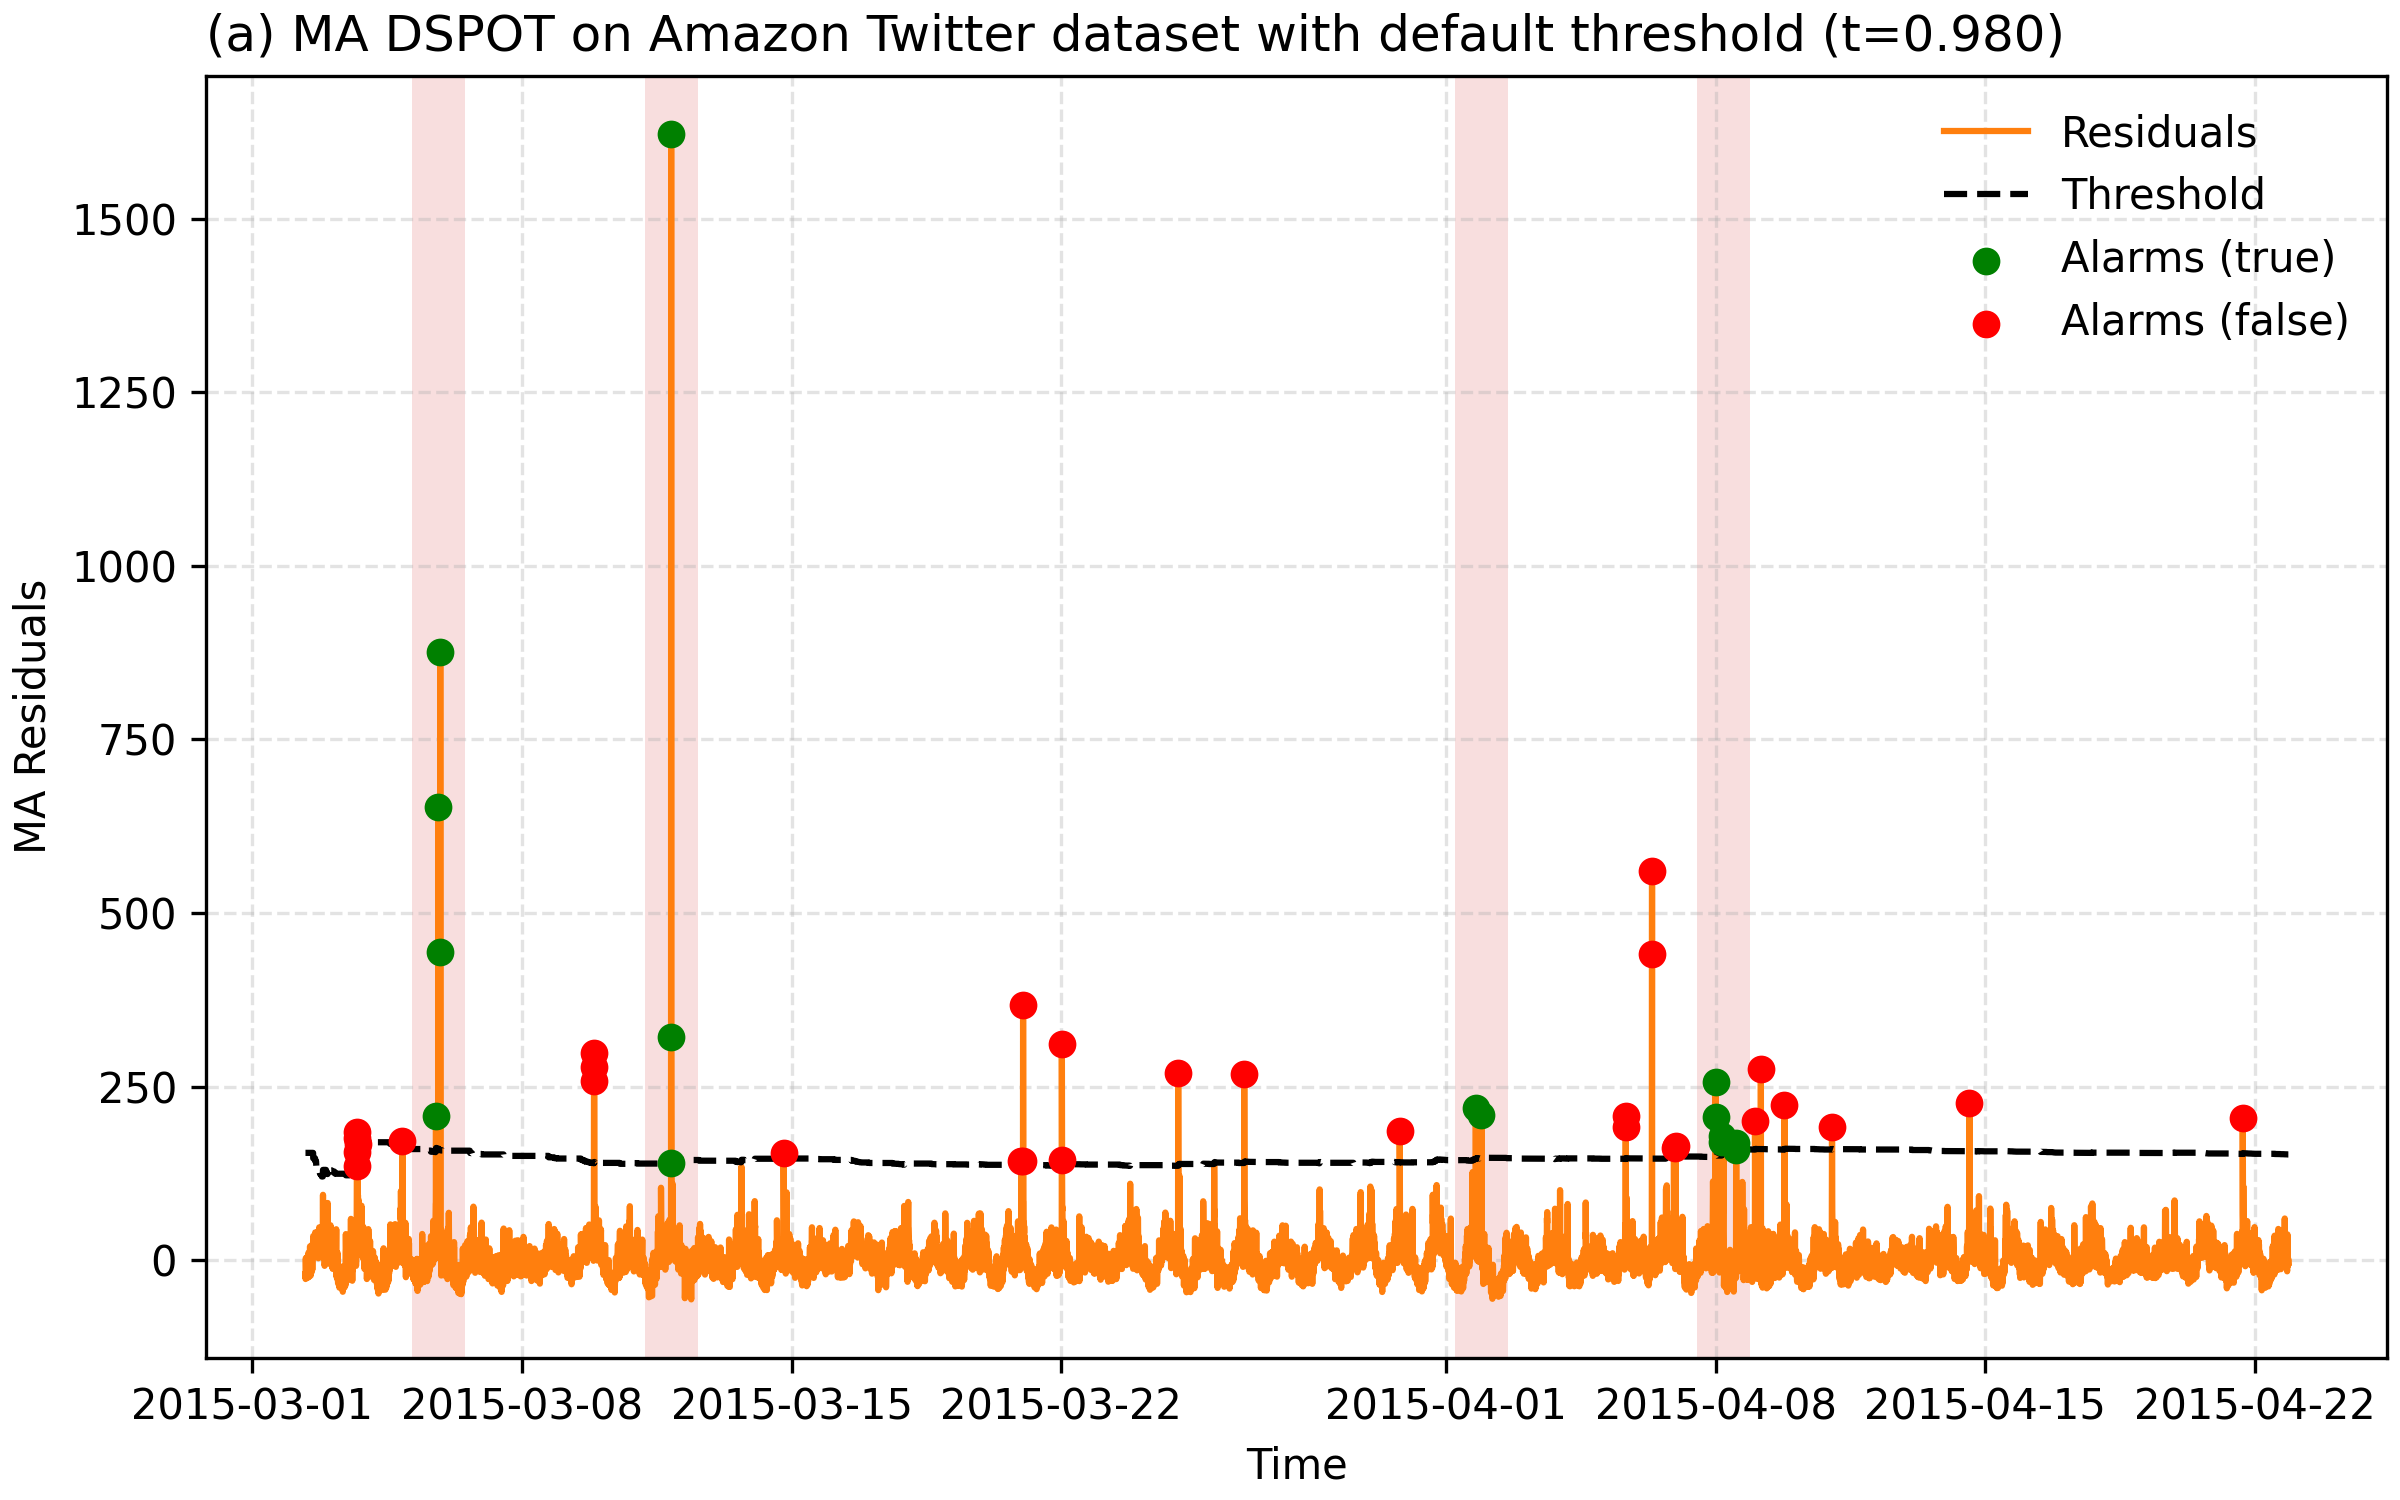
\includegraphics[width=\linewidth]{../output/realTweets/original_dspot_realTweets.png}
    \vspace{0.35em}
    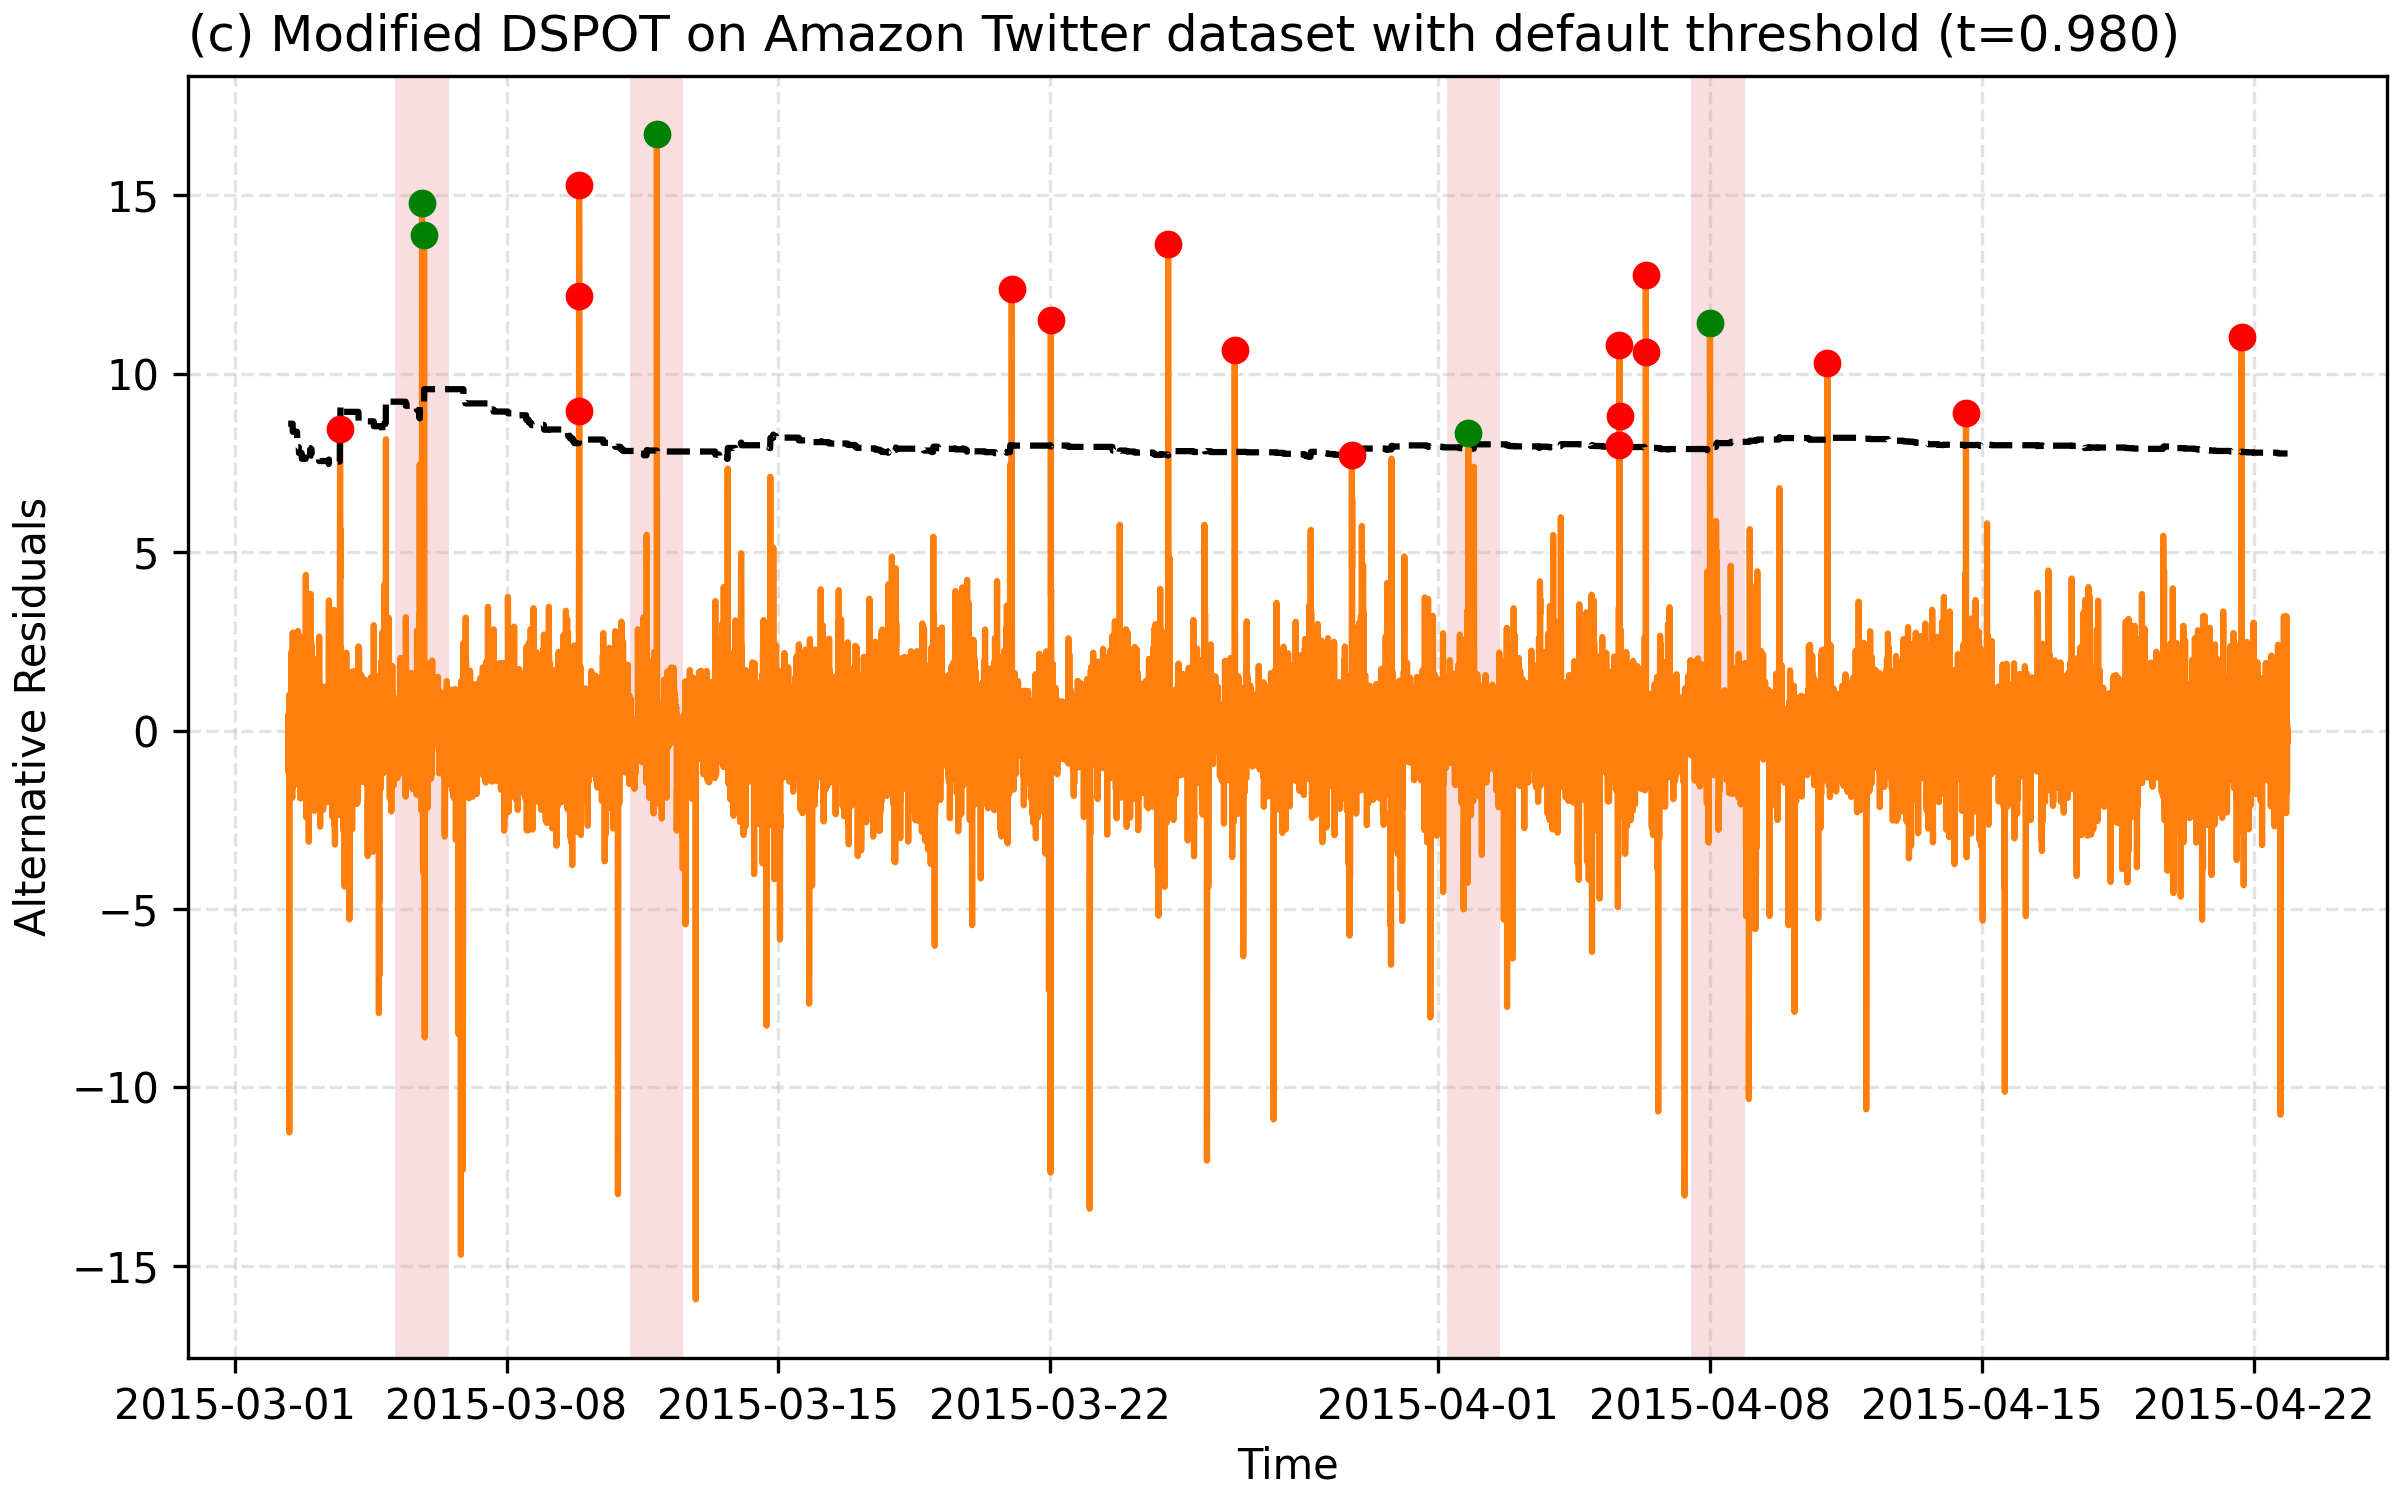
\includegraphics[width=\linewidth]{../output/realTweets/preprocessed_spot_realTweets.png}
  \end{minipage}\hfill
  \begin{minipage}{0.48\linewidth}
    \centering
    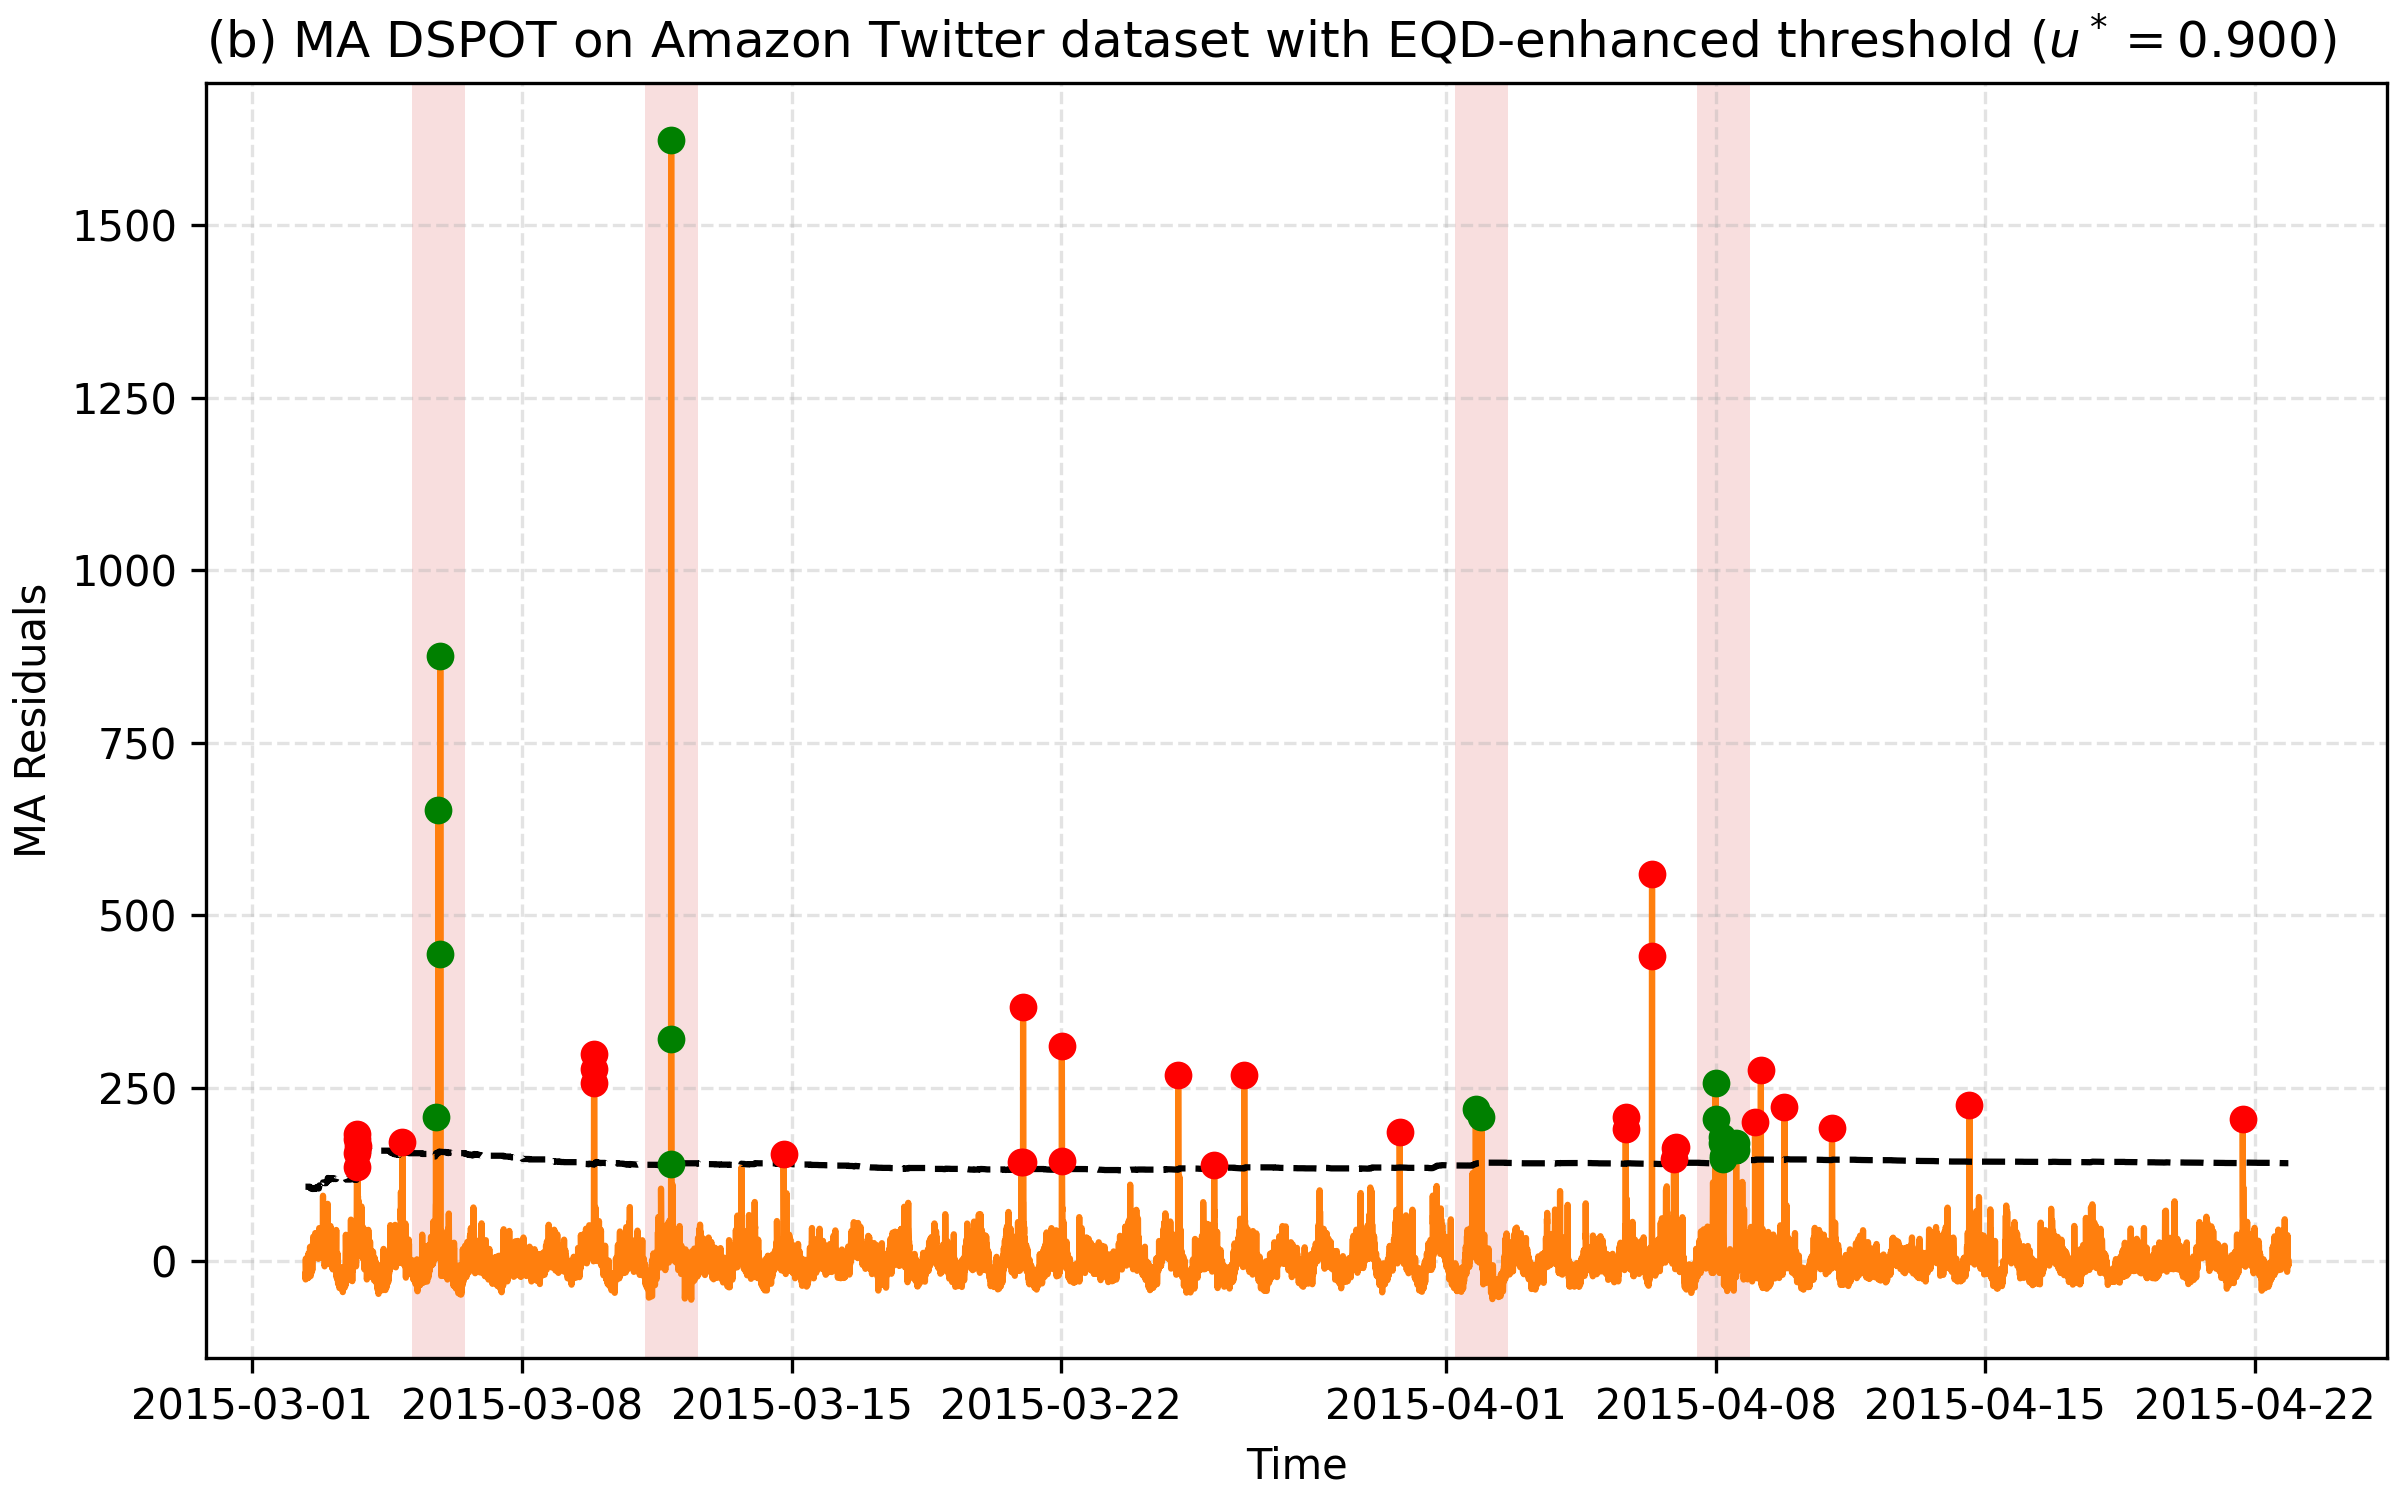
\includegraphics[width=\linewidth]{../output/realTweets/optimal_threshold_dspot_realTweets.png}
    \vspace{0.35em}
    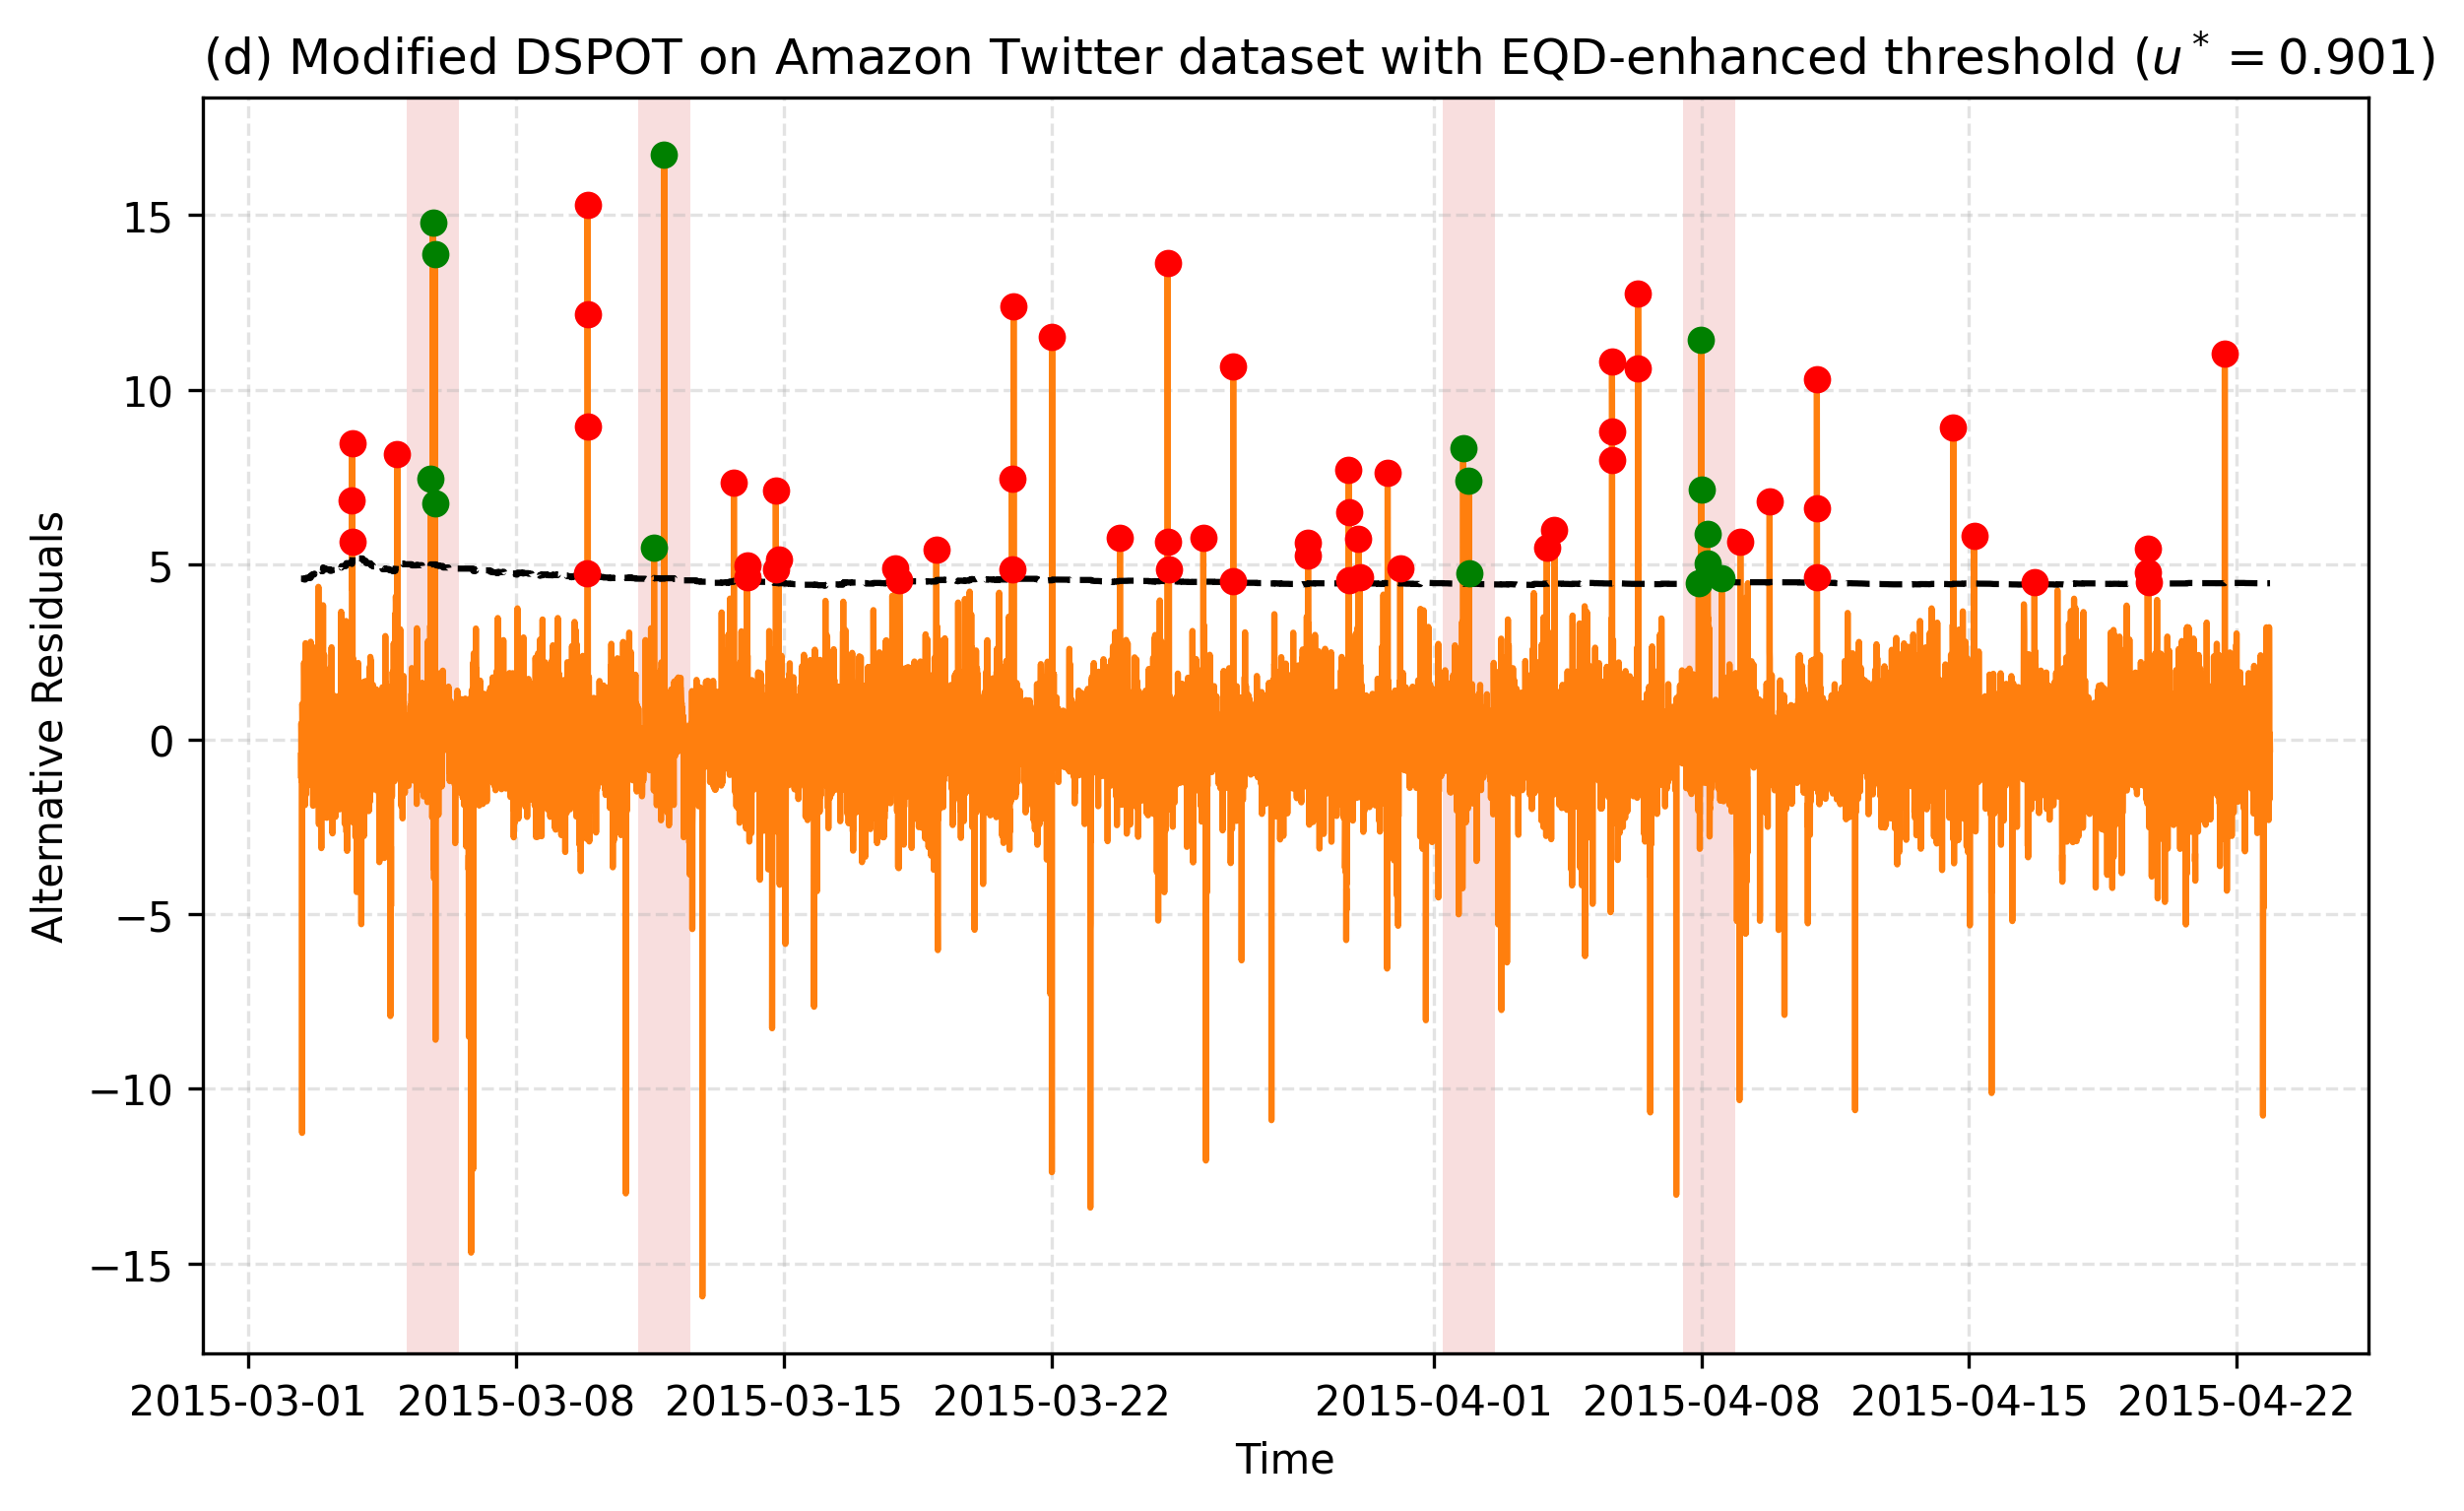
\includegraphics[width=\linewidth]{../output/realTweets/optimal_threshold_preprocessed_spot_realTweets.png}
  \end{minipage}
  \caption{Anomaly detection results on the Amazon Twitter dataset. 
  Each panel shows residuals, dynamic thresholds (dashed), and alarm events (dots) under the four DSPOT variants: 
  (a) MA residuals with default threshold, (b) MA residuals with EQD-enhanced threshold, 
  (c) alternative residuals with default threshold, and (d) alternative residuals with EQD-enhanced threshold. 
  Shaded bands indicate ground-truth anomaly windows.}
  \label{fig:evt_ad_twitter}
\end{figure}

\noindent\textbf{Amazon Twitter Volume.} The Twitter dataset presents a challenging case. 
As seen in Table~\ref{tab:amzn_event_metrics}, while the original DSPOT on MA residuals (a and b) detects all four events,
it suffers from very low precision (0.15–0.17). Since diagnostics for the MA residuals indicated that exceedances were not 
approximately i.i.d., EQD selects a lower threshold ($u^*=0.9$) and produces two additional false alarms, 
slightly reducing precision. In contrast, the modified DSPOT on alternative residuals (c) substantially improves precision (0.27), 
halving the false positives while maintaining full recall. This reflects the benefit of variance stabilisation and seasonal 
differencing in suppressing regular peaks. However, when EQD is combined with alternative residuals (d), the results degrade 
sharply: precision falls to 0.095 with a large number of false alarms. This outcome is consistent with the diagnostic finding
that the residuals remain far from i.i.d.. In such settings, EQD’s bias–variance trade-off is distorted, producing 
thresholds that are overly permissive for both preprocessing pipelines. Unlike in the CPU dataset, where anomalies were so 
distinct that permissive thresholds did not harm performance, here the weaker signal relative to baseline variability causes
a collapse in precision. Detection delays remain long (690–880 minutes) across all variants. In short, the Twitter data 
illustrate the limits of preprocessing when the i.i.d.\ assumption is strongly violated: improvements are possible, 
but gains are bounded. Figure~\ref{fig:evt_ad_twitter} further illustrates that alarms under both preprocessing pipelines 
occur in bursts, reflecting strong clustering of exceedances. This suggests that a natural next step in the preprocessing 
would be \emph{declustering}--grouping runs of exceedances into clusters and retaining only one representative value from each cluster,
so that the threshold model is fitted on approximately independent extremes \citep{Coles2001}. Here too, the Wilson confidence
intervals are wide, reflecting the small number of anomaly windows. Importantly, however, even the upper bounds on precision
remain modest (e.g. 0.52 for the best-performing variant), underscoring that poor precision is not simply an artefact of 
sampling variability but a consistent limitation across all models in this dataset.

\begin{table}[ht]
\centering
\caption{Event-based evaluation on the Amazon Twitter dataset (POT risk $q{=}10^{-3}$). Precision and recall show 95\% Wilson CIs.}
\label{tab:amzn_event_metrics}

% Local spacing tweaks (package-free)
\begingroup
\setlength{\tabcolsep}{4pt}        % default 6pt; tighter
\renewcommand{\arraystretch}{1.15} % row height
\footnotesize                      % or \scriptsize if you still overflow

\begin{tabular}{|l|r|r|r|c|c|c|c|}
\hline
Method & TP & FP & FN & Precision & Recall & F1 & Median Delay, min\\
\hline
a) DSPOT (default)
  & 4 & 20 & 0
  & \estci{0.167}{0.067}{0.359}
  & \estci{1.000}{0.510}{1.000}
  & 0.286 & 837.5 \\
b) DSPOT (EQD)
  & 4 & 22 & 0
  & \estci{0.154}{0.061}{0.335}
  & \estci{1.000}{0.510}{1.000}
  & 0.267 & 837.5 \\
c) Mod.DSPOT (default)
  & 4 & 11 & 0
  & \estci{0.267}{0.109}{0.520}
  & \estci{1.000}{0.510}{1.000}
  & 0.400 & 880.0 \\
d) Mod. DSPOT (EQD)
  & 4 & 38 & 0
  & \estci{0.095}{0.038}{0.221}
  & \estci{1.000}{0.510}{1.000}
  & 0.174 & 690.0 \\
\hline
\end{tabular}
\endgroup
\end{table}

\begin{figure}[ht]
  \centering

  \begin{minipage}{0.48\linewidth}
    \centering
    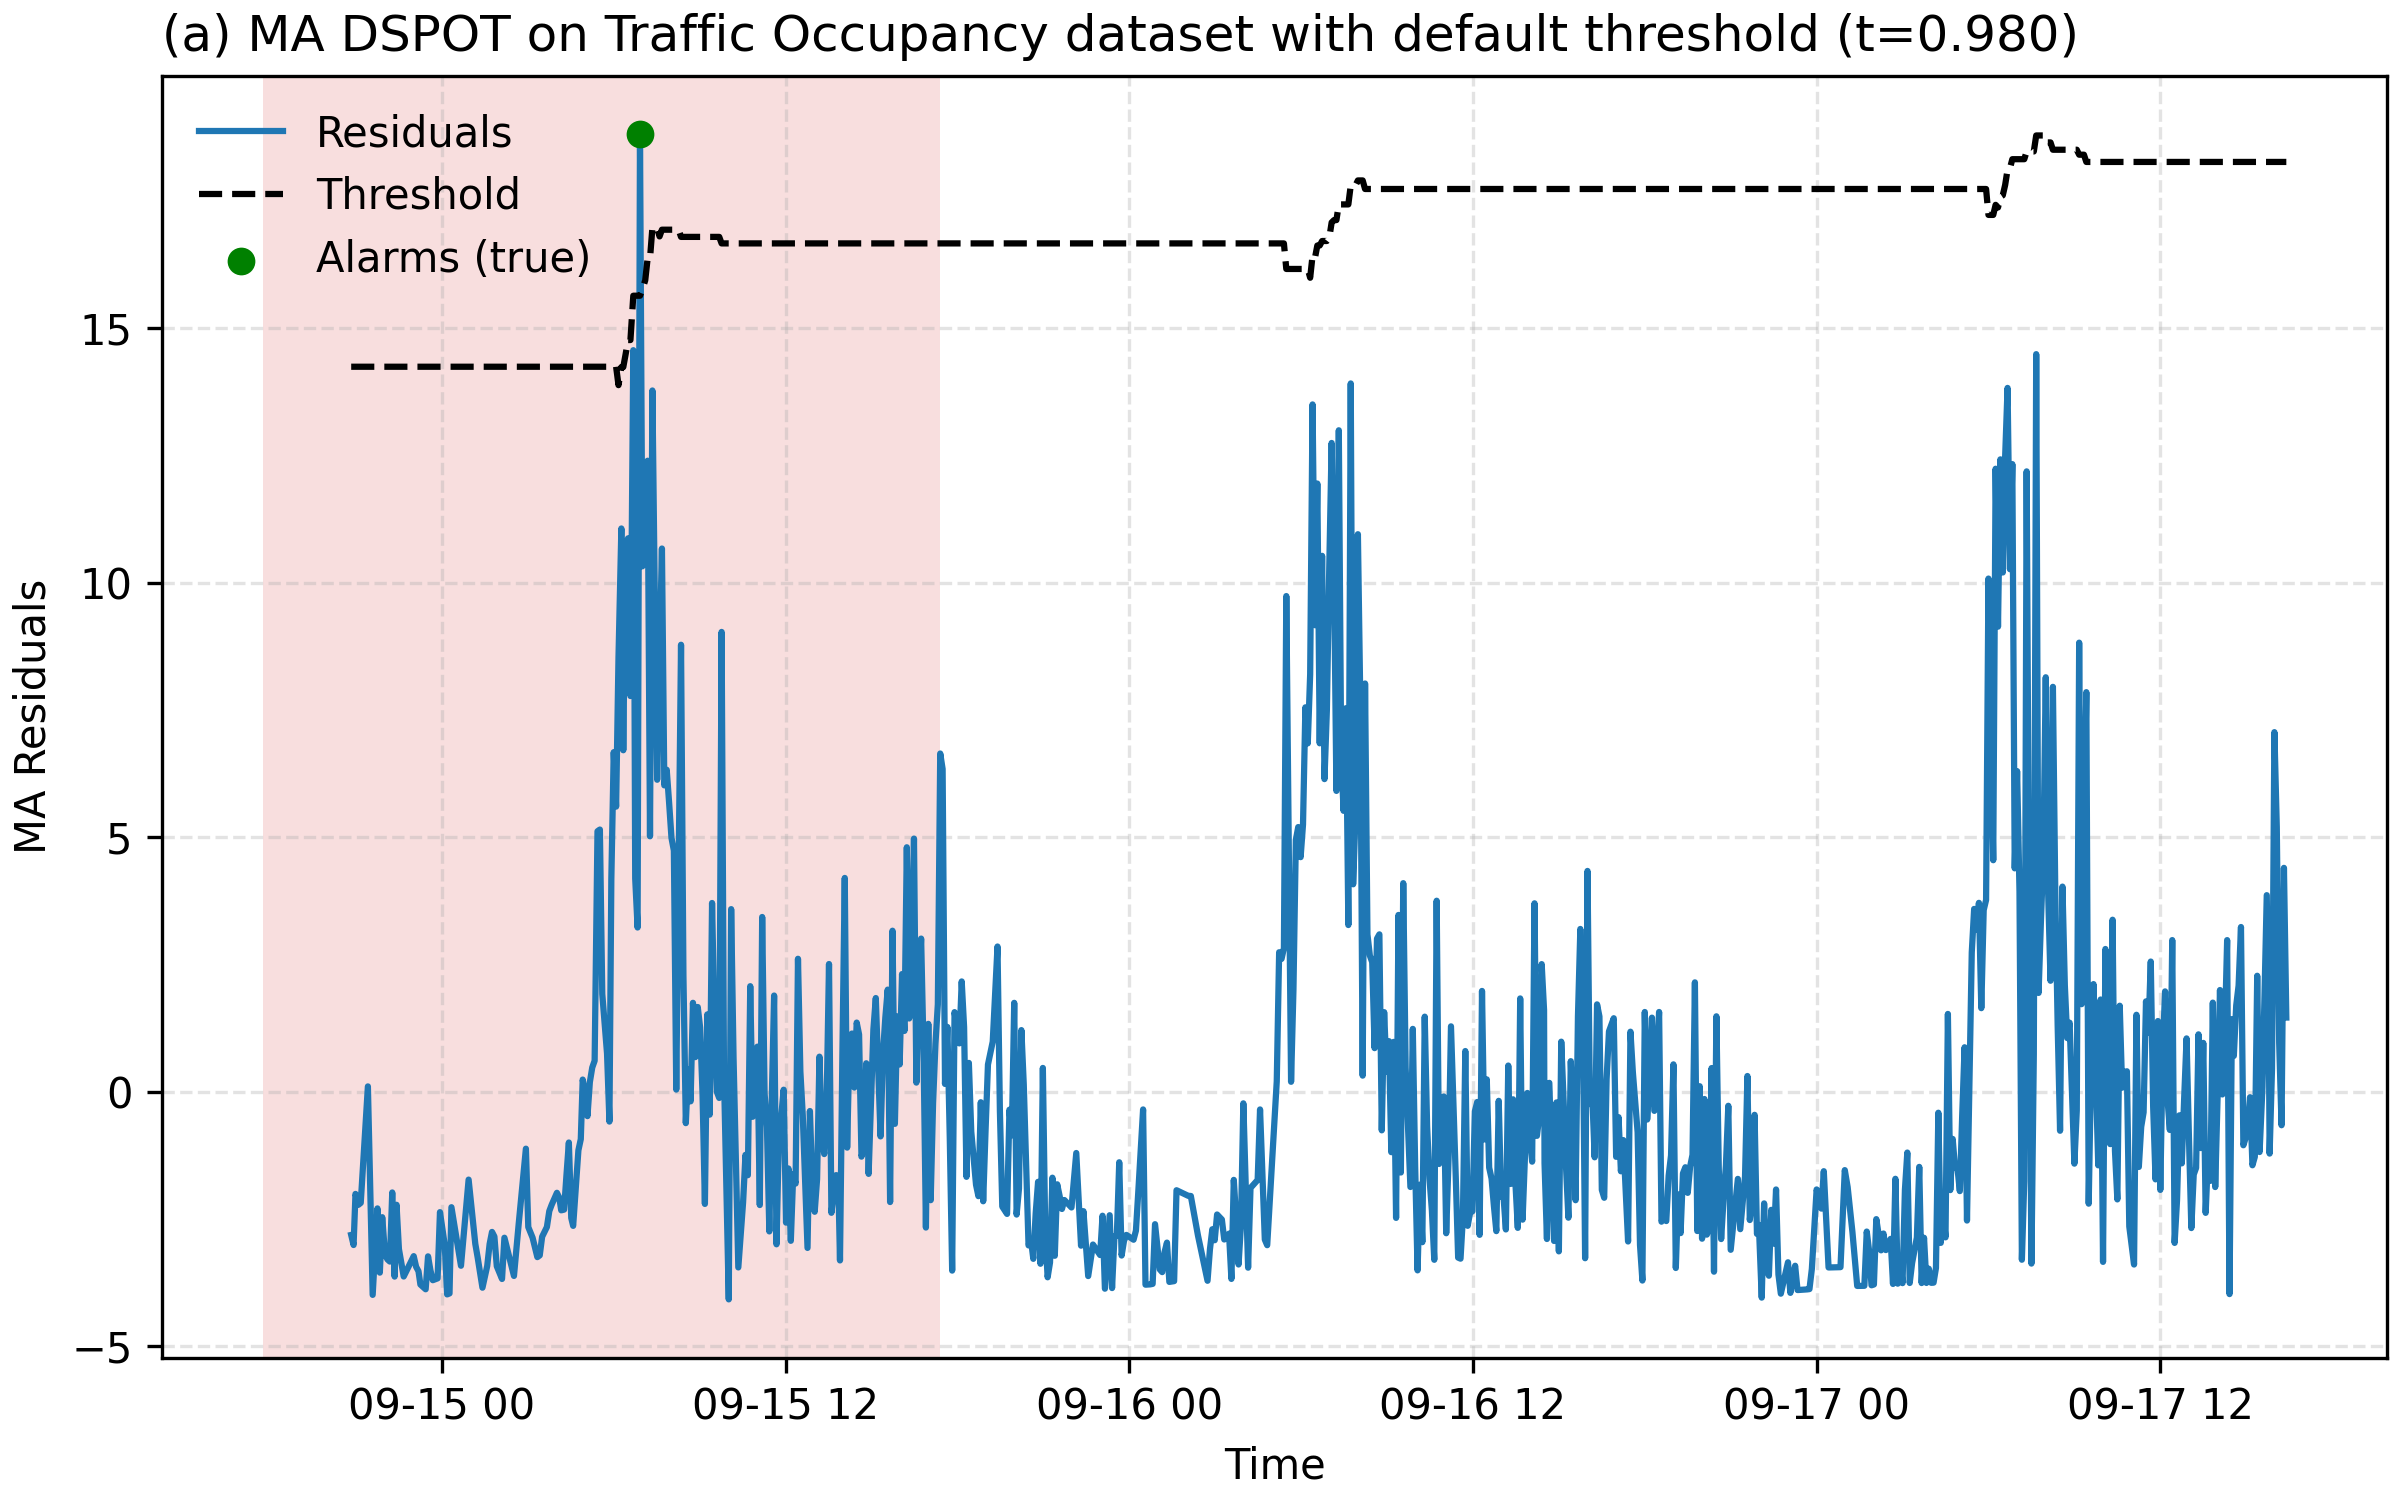
\includegraphics[width=\linewidth]{../output/occupancy/original_dspot_occupancy.png}
    \vspace{0.35em}
    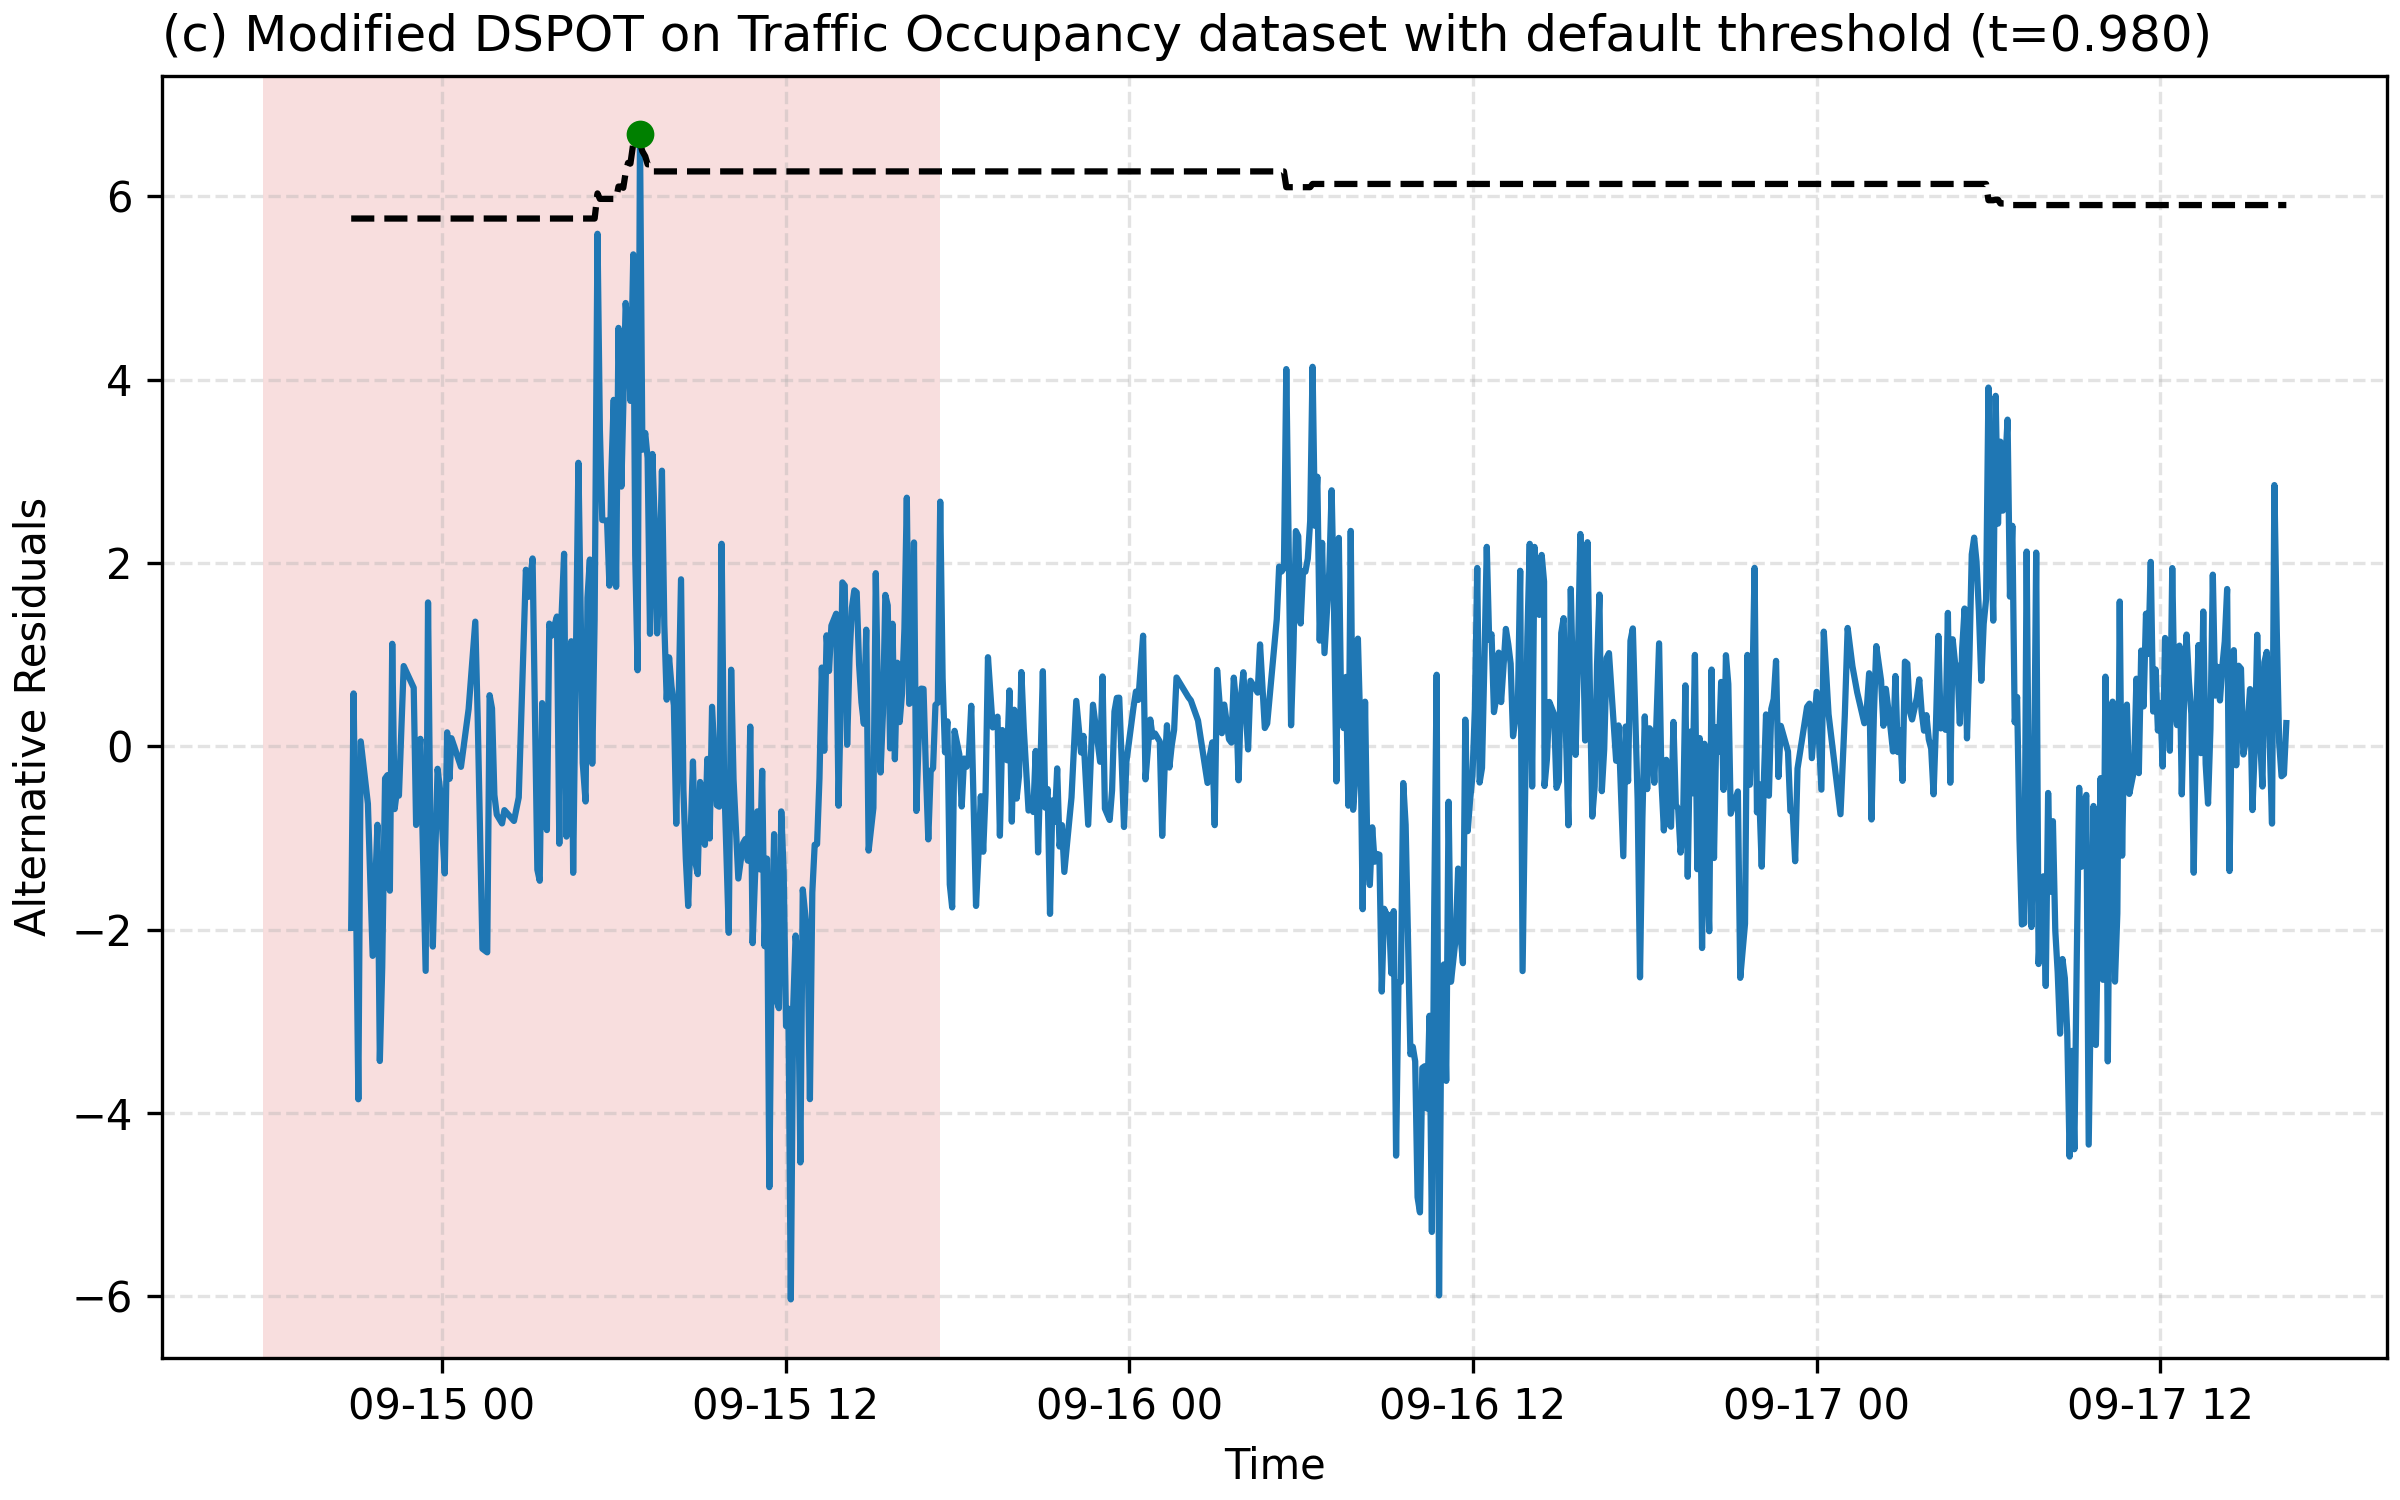
\includegraphics[width=\linewidth]{../output/occupancy/preprocessed_spot_occupancy.png}
  \end{minipage}\hfill
  \begin{minipage}{0.48\linewidth}
    \centering
    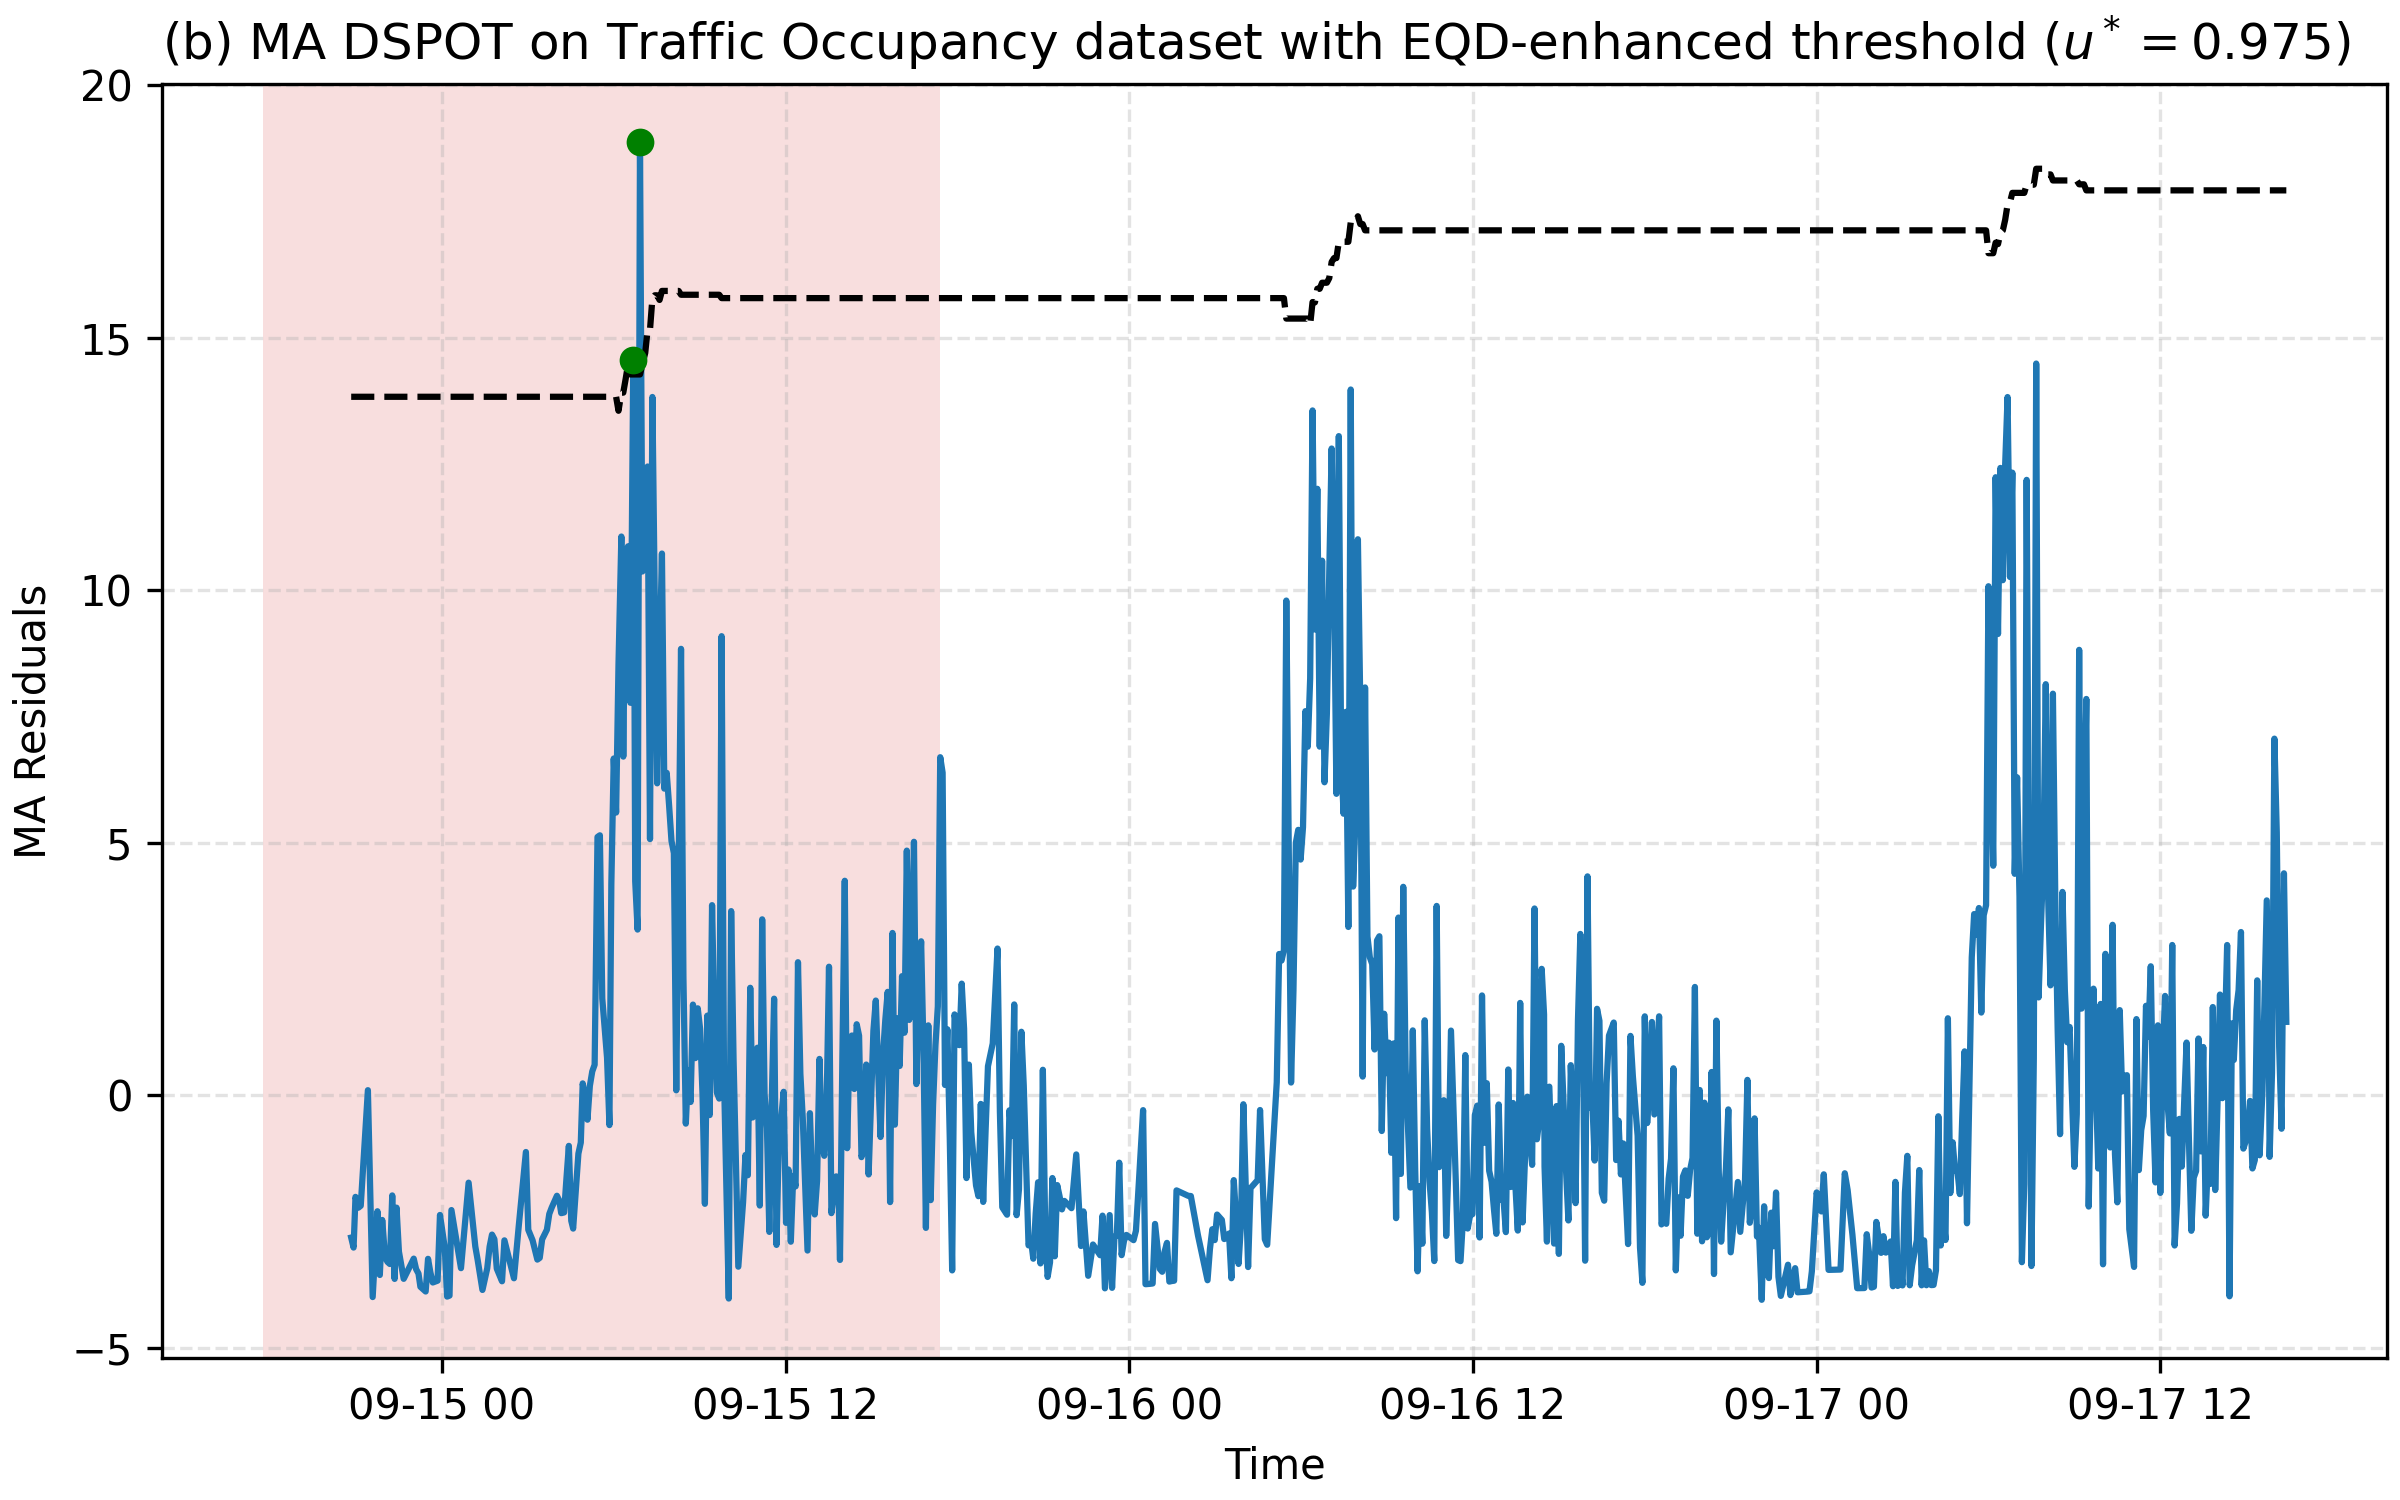
\includegraphics[width=\linewidth]{../output/occupancy/optimal_threshold_dspot_occupancy.png}
    \vspace{0.35em}
    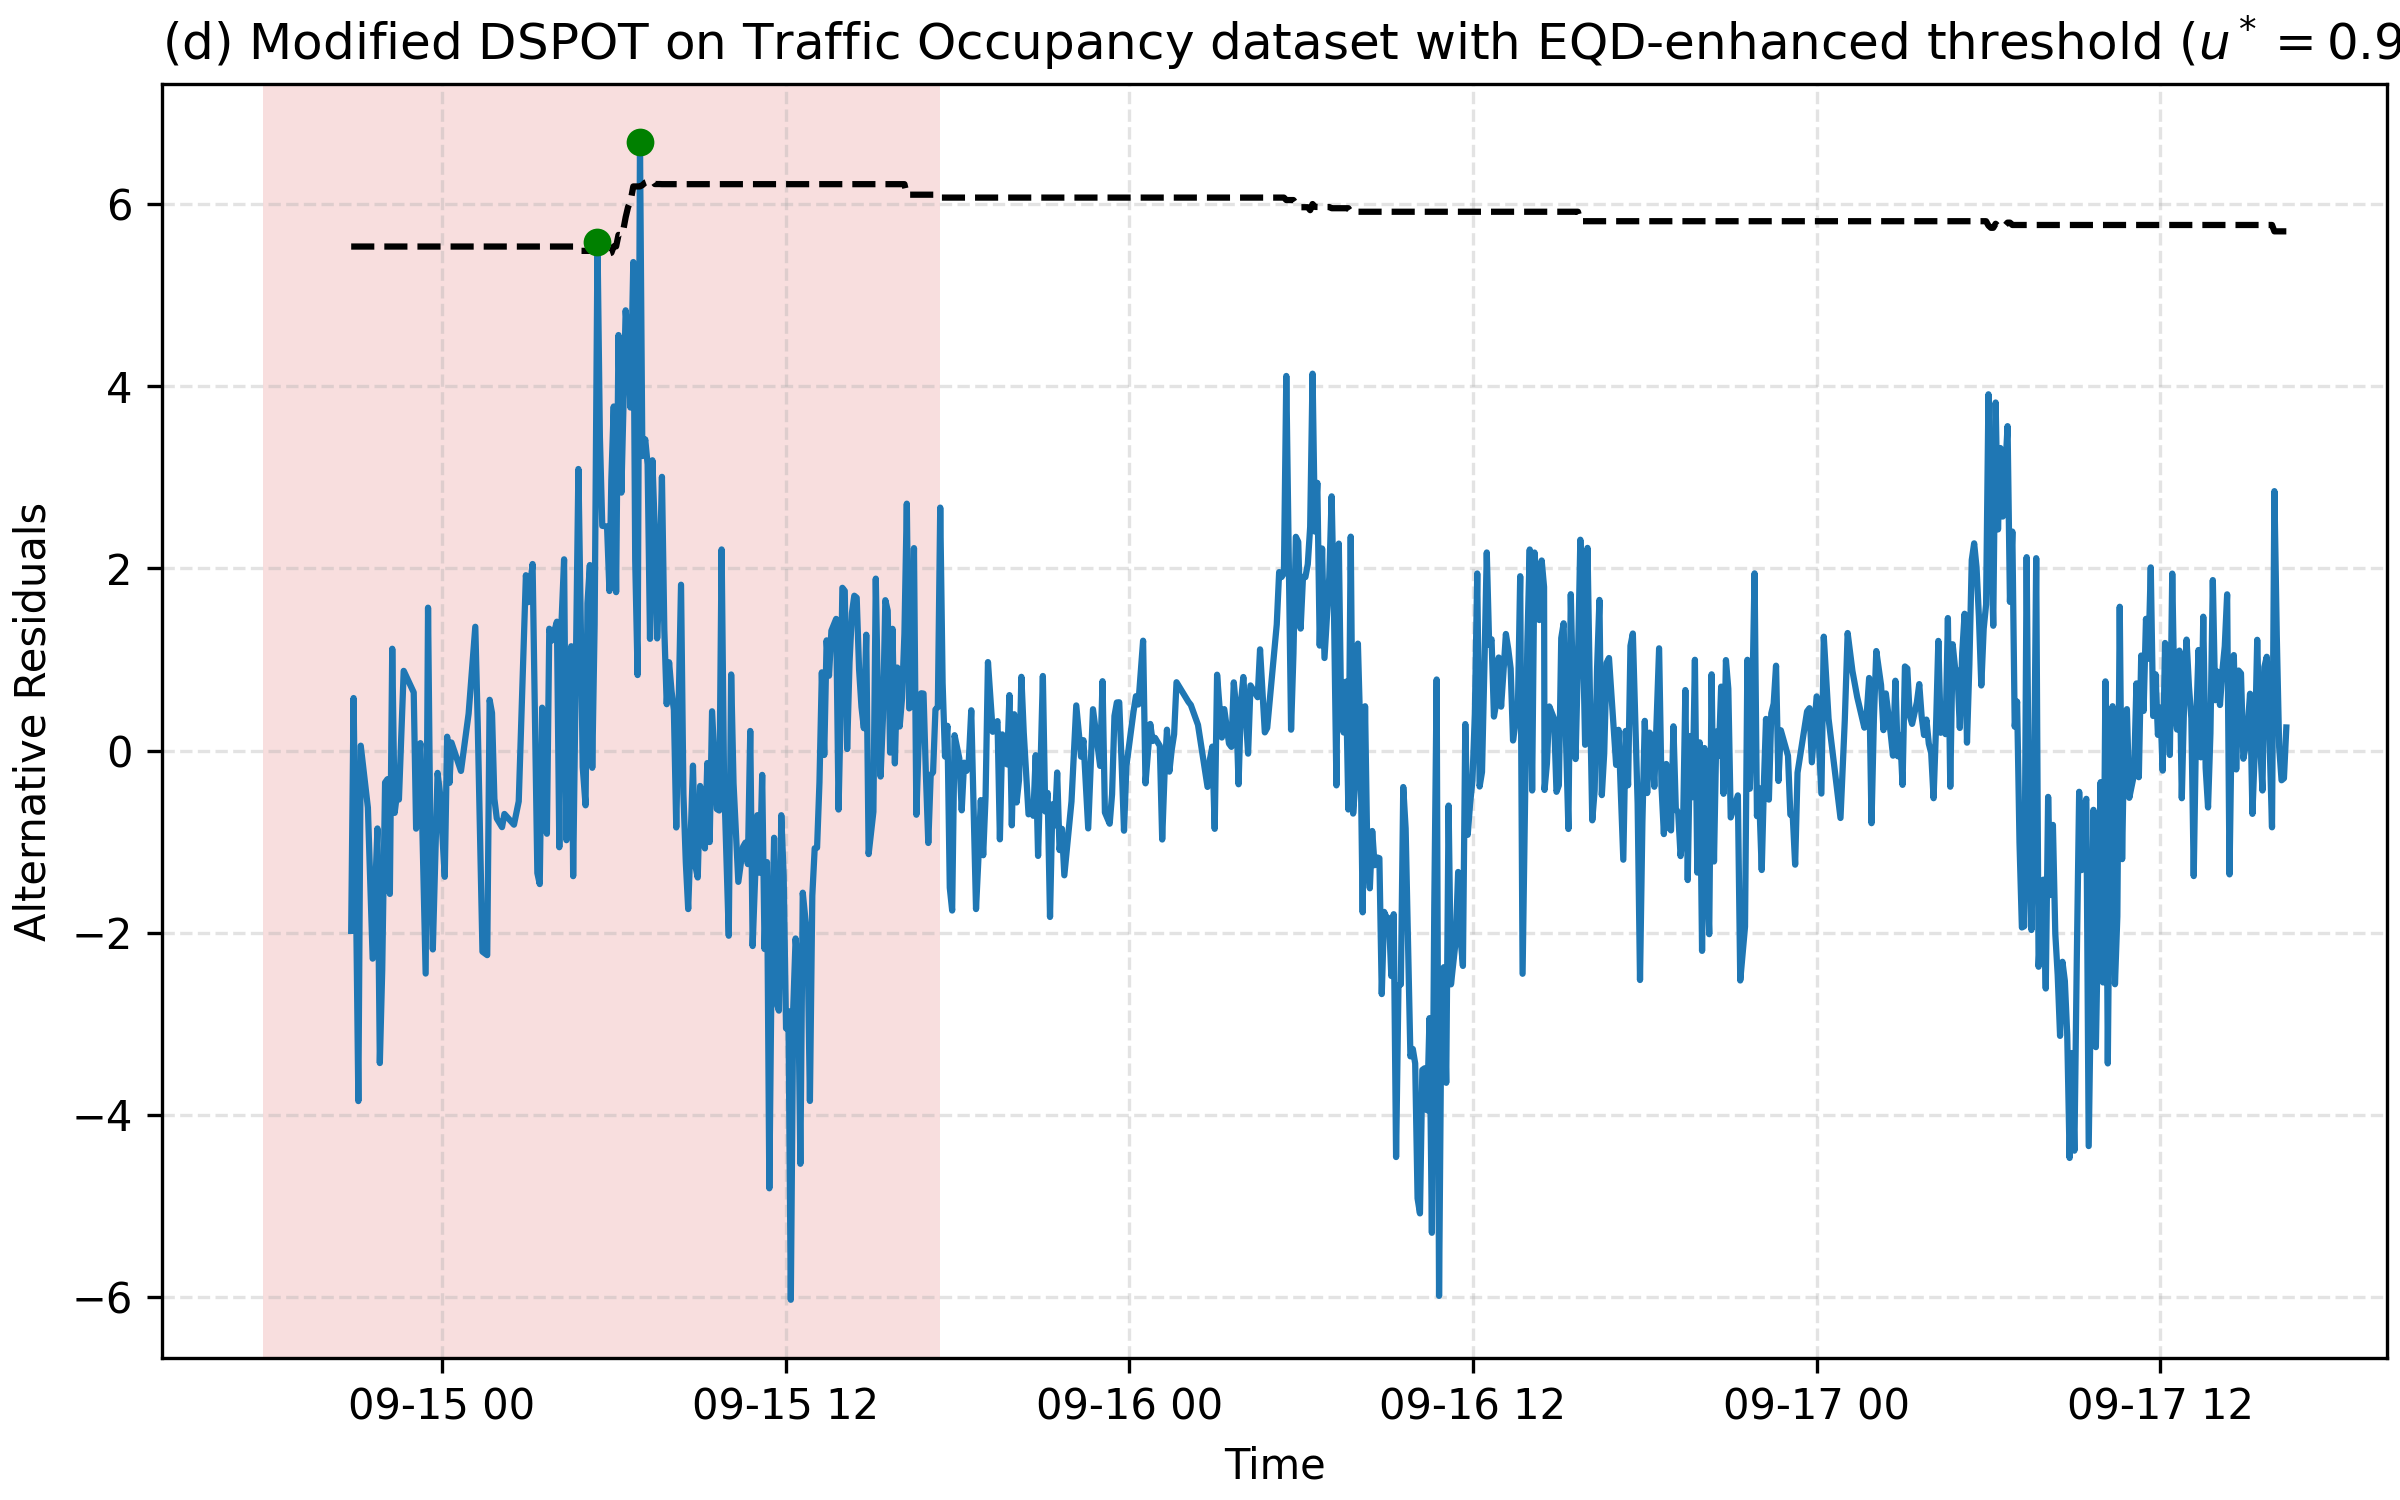
\includegraphics[width=\linewidth]{../output/occupancy/optimal_threshold_preprocessed_spot_occupancy.png}
  \end{minipage}
  \caption{Anomaly detection results on the Traffic Occupancy dataset. 
  Each panel shows residuals, dynamic thresholds (dashed), and alarm events (dots) under the four DSPOT variants: 
  (a) MA residuals with default threshold, (b) MA residuals with EQD-enhanced threshold, 
  (c) alternative residuals with default threshold, and (d) alternative residuals with EQD-enhanced threshold.
  Shaded bands indicate ground-truth anomaly windows.}
  \label{fig:evt_ad_traffic}
\end{figure}

\noindent\textbf{Traffic Occupancy.} The Traffic dataset, with strong daily periodicity and marked heteroskedasticity, 
is the setting most favourable to the 
enhanced pipeline. All four DSPOT variants achieve perfect classification of the two anomaly windows (no FPs or FNs; 
Table~\ref{tab:traffic_event_metrics}). However, the Wilson intervals ([0.207, 1.000]) again reflect the large uncertainty
inherent in evaluating a single anomaly event, so even seemingly perfect results should be interpreted with caution. 
The only dimension that distinguishes methods is detection delay.
Median delays are 790 minutes for (a) DSPOT (MA, default), 776 minutes for (b) DSPOT (MA, EQD), 790 minutes for (c) 
modified DSPOT (alternative, default), and 701 minutes for (d) modified DSPOT (alternative, EQD).
Sncie methods  (a) and (c) have the same median delay, alternative preprocessing alone does not improve timeliness. 
In contrast, EQD yields a modest reduction on MA residuals (a$\to$b: $-14$ minutes) and a more substantial reduction when 
paired with the alternative residuals (c$\to$d: $-89$ minutes). Given that anomaly windows span many hours, these reductions
are moderate in relative terms but practically important: earlier threshold crossings advance the first alarm within wide 
events. This pattern is consistent with the diagnostics, which indicated that the alternative residuals came closest 
to approximate independence (Figure~\ref{fig:prep_occupancy}); under those conditions, EQD’s threshold refinement 
is better calibrated and can bring forward detection, even though classification accuracy is already saturated at 100\%.

\begin{table}[ht]
\centering
\caption{Event-based evaluation on the Traffic Occupancy dataset (POT risk $q{=}10^{-3}$). 
All methods achieve perfect classification (Precision = Recall = F1 = 1.000 [0.207, 1.000]); 
the only difference lies in detection delays.}
\label{tab:traffic_event_metrics}

\begingroup
\setlength{\tabcolsep}{4pt}        % default 6pt; tighter
\renewcommand{\arraystretch}{1.15} % row height
\footnotesize

\begin{tabular}{|l|c|}
\hline
Method & Median Delay, min \\
\hline
a) DSPOT (default)        & 790 \\
b) DSPOT (EQD)            & 776 \\
c) Mod. DSPOT (default)   & 790 \\
d) Mod. DSPOT (EQD)       & 701 \\
\hline
\end{tabular}
\endgroup
\end{table}

\section{Discussion}\label{sec:discussion}

This study examined how Extreme Value Theory (EVT), in particular the Peaks-Over-Threshold (POT) framework, can be adapted 
for anomaly detection in non-stationary data streams. This work addressed the problem in two main ways: by developing a 
richer preprocessing pipeline aimed at producing residuals that come closer to EVT’s weak-dependence requirements, and by
introducing the Expected Quantile Discrepancy (EQD) as a data-driven tool for threshold selection. The main conclusion is
that POT-based detectors remain feasible in streaming contexts, but their reliability depends on how far preprocessing can
reduce dependence in the extremes. Approximate independence is not always achieved, yet the closer the exceedances come to
this condition, the more stable and interpretable the resulting thresholds become. EQD-based threshold selection provides 
an additional layer of stability, though only when residual extremes already approximate independence. Where this assumption
is not met, the procedure can even deteriorate performance. 

In more detail, the empirical results show that the three benchmark datasets exhibit distinct types of non-stationarity--mean shifts in CPU,
clear daily cycles in Traffic, and bursty clustering in Twitter--with direct consequences for both preprocessing and the 
validity of POT modelling. For the CPU Utilisation series, where the main issue was a single mean shift, the moving average 
(MA) residuals were sufficient: they reduced short-range dependence and preserved a well-calibrated GPD tail fit. 
The Traffic Occupancy dataset, by contrast, contained strong daily cycles and moderate variation in peak intensity. Here the 
MA pipeline already yielded a reasonably good tail model, but residual dependence persisted. The alternative pipeline brought
clearer gains, further reducing dependence while maintaining an excellent GPD fit. For both preprocessing pipelines, EQD
shortened detection delay without altering classification outcomes. The Twitter dataset was the most difficult case: both 
preprocessing pipelines improved variance stability, but neither removed the heavy dependence and clustering of extremes, 
and EQD then tended to worsen calibration.

These findings connect directly to the broader anomaly-detection literature. Relative to SPOT and DSPOT 
\citep{siffer2017anomaly}, the present results make clear that preprocessing and thresholding choices are not secondary details
but central to robustness. EVT remains attractive because it delivers interpretable thresholds with a direct probabilistic 
meaning, yet this advantage diminishes once residual dependence is left unresolved. A further nuance is that EVT-based 
detectors are intrinsically tuned to extremes: they are well suited for identifying unusually large deviations, but may 
overlook anomalies that are subtle or not extreme in scale. By contrast, the machine-learning approaches for streaming 
data outlined in Section~\ref{subsec:challenges} are often better at adjusting to changing distributions and can pick up
a wider range of patterns. What they usually do not provide, however, is any clear control over false-alarm rates. Taken
together, these comparisons suggest that EVT remains competitive when anomalies manifest as extremes and preprocessing 
succeeds in reducing dependence, while ML methods cover a broader range of behaviours at the cost of statistical guarantees.

One broader lesson concerns the trade-off between independence and tail fidelity. The MA pipeline tended to preserve the 
natural scale of extremes, at the expense of residual dependence. The alternative pipeline reduced dependence more effectively,
but at times compressed genuine extremes, which weakened the GPD fit. This type of tension is not unique to streaming contexts:
in classical EVT, it is well recognised that detrending, deseasonalising, or stabilising variance can alter the behaviour of 
extremes, sometimes reducing the information available for tail inference \citep{EastoeTawn2009}. What is novel
here is the explicit quantification of this trade-off in a streaming setting. The results suggest that robustness depends not
only on reducing non-stationarity but also on avoiding distortions of the very extremes that EVT seeks to model. To our 
knowledge, this thesis provides one of the first systematic demonstrations of this trade-off in a streaming EVT setting, 
offering a new perspective on how preprocessing choices shape the feasibility of POT-based anomaly detection.

The results must also be read in light of small-sample uncertainty. Each dataset contained at most four anomaly windows, 
meaning that Wilson confidence intervals around precision and recall estimates were often wide. These intervals should 
therefore be interpreted as rough indicators rather than precise bounds. Even so, they remain informative: in the CPU dataset,
the intervals already hint at systematic differences between methods, with default DSPOT variants showing consistently higher
precision and recall than the modified pipeline. In the Twitter dataset, by contrast, the intervals largely overlapped across
methods, reflecting that all approaches suffered from low precision driven by many false positives. It is therefore important
to interpret these results cautiously, as small-sample metrics can suggest significance where none truly exists.

Three limitations of this work deserve emphasis. Foremost, the persistence of extremal clustering in the Twitter dataset shows
that preprocessing alone cannot always deliver i.i.d.\ exceedances. Classical EVT deals with this through declustering, 
and an online variant of that idea could bring the streaming approach closer to theoretical validity. Next, the CPU results
illustrated that heavy normalisation sometimes compressed genuine extremes, making anomalies less visible. This underlines
an important point: stronger preprocessing is not automatically an improvement. Finally, the NAB datasets impose practical 
limits. With only a handful of anomaly windows in each series, statistical power is low, and it becomes difficult to separate
genuine differences in performance from noise. Each of these limitations points toward areas where more systematic follow-up
work would be valuable.

A related point is the question of how thresholds relate back to the original measurement scale. In principle, 
the EVT quantiles estimated in the stationary $z$-difference domain can be projected back into raw units. We explored
this mapping for the alternative preprocessing pipeline, but the resulting curves were highly sensitive to small fluctuations
in the rolling mean and variance, and therefore appeared visually unstable. Since the purpose of these figures is to convey
the detector’s behaviour clearly, we chose to present thresholds only in the transformed space where the EVT model is defined.

Looking forward, two extensions appear particularly promising. The first is to embed declustering directly into DSPOT. 
An online runs-based rule that identifies clusters of exceedances and updates the GPD only with cluster maxima would align
the tail model more closely with EVT’s independence requirements while still allowing immediate alarms. The second is to 
place POT-based detectors in direct comparison with modern ML methods under controlled benchmarks. A comparison of this 
kind would move past the informal contrasts that exist so far and make it possible to evaluate, in a more systematic way,
the trade-offs between EVT’s interpretability and ML’s adaptability. Taken together, these two lines of work would advance
the methodology and, at the same time, enhance its practical value.

In plain terms, this work shows that statistical tools for extremes still have a place in today’s fast, evolving data streams.
With the right preprocessing, they can provide reliable alarms with clear error rates. The challenge ahead is 
to combine their statistical rigour with the flexibility of newer machine-learning tools, so that anomaly detection becomes
both trustworthy and adaptable.

\section{Endmatter}\label{sec:endmatter}

\paragraph{Data availability.} 
All datasets analysed in this thesis are publicly available through the Numenta Anomaly Benchmark (NAB) framework
\citep{lavin2015evaluating}, which can be accessed at \url{https://github.com/numenta/NAB/tree/master}. 
The raw series and ground-truth anomaly windows used in this study are included there in full.

\paragraph{Reproducibility.} 
The code developed for this thesis, including preprocessing pipelines, thresholding implementations, and evaluation 
routines, is made openly available at:  
\url{https://github.com/kkquest/msc_thesis}.  
This repository contains scripts and instructions needed to reproduce all figures and results reported in the thesis. 
To support readability and reproducibility, comments within the final code were edited with the help of GPT-5, while 
the design and implementation of all methods remained the author’s own work.

\paragraph{Use of Large language models (LLMs).} 
LLMs were used in this project in a limited and responsible way. GPT-5, accessed via the ChatGPT graphical interface, 
assisted with copy-editing the abstract and endmatter, editing code comments for clarity (as mentioned above), and supporting 
literature searches. Grammarly was used to improve the quality of written English. All statistical modelling, 
coding, analysis, and substantive interpretation were carried out independently by the author.


%=========================================================
%
%
%
% Students should not edit below here 
%
%
%
%=========================================================

%=========================================================
%% Create bibliography
%
% - Add your references by modifying the file `refs.bib`
%
%=========================================================

\clearpage
%% reset page counter and start appendix pages numbering
\pagenumbering{arabic}
\renewcommand*{\thepage}{References | Page \arabic{page}}

%%References part of the main text
% References: modify the file refs.bib
\bibliographystyle{apalike}
\bibliography{refs}

\clearpage

%=========================================================
%% Create supplementary material 
%
%
% - Providing supplementary materials to your report is voluntary and will not normally be read by your examiners.
% - If you wish to include supplementary materials, add these by modifying the file 
%   `supplementary.tex`
% - otherwise deactive the include command below
%
%
%=========================================================

%% reset page counter and start appendix pages numbering
\pagenumbering{arabic}
\renewcommand*{\thepage}{Supplementary Material | Page \arabic{page}}
\renewcommand{\thesection}{\Alph{section}}
%% Supplementary Material goes here
\appendix
\pagebreak

\section{Theorems}\label{sec:theorems}

\subsection{Fisher–Tippett–Gnedenko Theorem}\label{subsec:theorem_gev}
For completeness, we state below the Fisher–Tippett–Gnedenko theorem, which forms the foundation of block-maxima approaches in EVT. 
We omit the proof, which can be found in standard references such as 
\citet{gnedenko1943distribution} and \citet{Coles2001}.


\begin{theorem}[Fisher–Tippett–Gnedenko] \label{thm:gev}
Let \( X_1, \ldots, X_n \sim F \) i.i.d., and define \( M_n = \max(X_1, \ldots, X_n) \). 
If sequences \( {a_n} > 0 \), \( {b_n} \in \mathbb{R} \) exist such that
\begin{equation}
\frac{M_n - b_n}{a_n} \xrightarrow{d} G_\gamma(x),
\label{eqn:gev-limit}
\end{equation}
then the limiting distribution \( G_\gamma(x) \) belongs to the \textbf{Generalised Extreme Value (GEV)} family:
\begin{equation}
G_\gamma(x) = \exp\left\{ -\left(1 + \gamma \frac{x - \mu}{\sigma} \right)^{-1/\gamma} \right\}, 
\quad 1 + \gamma \frac{x - \mu}{\sigma} > 0,
\label{eqn:gev}
\end{equation}
where \( \mu \in \mathbb{R} \), \( \sigma > 0 \) and \( \gamma \in \mathbb{R} \) 
are location, scale and shape parameters, respectively.
\end{theorem}

%=========================================================


\end{document}
